\documentclass[]{book}
\usepackage{lmodern}
\usepackage{amssymb,amsmath}
\usepackage{ifxetex,ifluatex}
\usepackage{fixltx2e} % provides \textsubscript
\ifnum 0\ifxetex 1\fi\ifluatex 1\fi=0 % if pdftex
  \usepackage[T1]{fontenc}
  \usepackage[utf8]{inputenc}
\else % if luatex or xelatex
  \ifxetex
    \usepackage{mathspec}
  \else
    \usepackage{fontspec}
  \fi
  \defaultfontfeatures{Ligatures=TeX,Scale=MatchLowercase}
\fi
% use upquote if available, for straight quotes in verbatim environments
\IfFileExists{upquote.sty}{\usepackage{upquote}}{}
% use microtype if available
\IfFileExists{microtype.sty}{%
\usepackage{microtype}
\UseMicrotypeSet[protrusion]{basicmath} % disable protrusion for tt fonts
}{}
\usepackage{hyperref}
\hypersetup{unicode=true,
            pdftitle={Introduction to R},
            pdfauthor={Sarah Bonnin},
            pdfborder={0 0 0},
            breaklinks=true}
\urlstyle{same}  % don't use monospace font for urls
\usepackage{natbib}
\bibliographystyle{apalike}
\usepackage{color}
\usepackage{fancyvrb}
\newcommand{\VerbBar}{|}
\newcommand{\VERB}{\Verb[commandchars=\\\{\}]}
\DefineVerbatimEnvironment{Highlighting}{Verbatim}{commandchars=\\\{\}}
% Add ',fontsize=\small' for more characters per line
\usepackage{framed}
\definecolor{shadecolor}{RGB}{248,248,248}
\newenvironment{Shaded}{\begin{snugshade}}{\end{snugshade}}
\newcommand{\AlertTok}[1]{\textcolor[rgb]{0.94,0.16,0.16}{#1}}
\newcommand{\AnnotationTok}[1]{\textcolor[rgb]{0.56,0.35,0.01}{\textbf{\textit{#1}}}}
\newcommand{\AttributeTok}[1]{\textcolor[rgb]{0.77,0.63,0.00}{#1}}
\newcommand{\BaseNTok}[1]{\textcolor[rgb]{0.00,0.00,0.81}{#1}}
\newcommand{\BuiltInTok}[1]{#1}
\newcommand{\CharTok}[1]{\textcolor[rgb]{0.31,0.60,0.02}{#1}}
\newcommand{\CommentTok}[1]{\textcolor[rgb]{0.56,0.35,0.01}{\textit{#1}}}
\newcommand{\CommentVarTok}[1]{\textcolor[rgb]{0.56,0.35,0.01}{\textbf{\textit{#1}}}}
\newcommand{\ConstantTok}[1]{\textcolor[rgb]{0.00,0.00,0.00}{#1}}
\newcommand{\ControlFlowTok}[1]{\textcolor[rgb]{0.13,0.29,0.53}{\textbf{#1}}}
\newcommand{\DataTypeTok}[1]{\textcolor[rgb]{0.13,0.29,0.53}{#1}}
\newcommand{\DecValTok}[1]{\textcolor[rgb]{0.00,0.00,0.81}{#1}}
\newcommand{\DocumentationTok}[1]{\textcolor[rgb]{0.56,0.35,0.01}{\textbf{\textit{#1}}}}
\newcommand{\ErrorTok}[1]{\textcolor[rgb]{0.64,0.00,0.00}{\textbf{#1}}}
\newcommand{\ExtensionTok}[1]{#1}
\newcommand{\FloatTok}[1]{\textcolor[rgb]{0.00,0.00,0.81}{#1}}
\newcommand{\FunctionTok}[1]{\textcolor[rgb]{0.00,0.00,0.00}{#1}}
\newcommand{\ImportTok}[1]{#1}
\newcommand{\InformationTok}[1]{\textcolor[rgb]{0.56,0.35,0.01}{\textbf{\textit{#1}}}}
\newcommand{\KeywordTok}[1]{\textcolor[rgb]{0.13,0.29,0.53}{\textbf{#1}}}
\newcommand{\NormalTok}[1]{#1}
\newcommand{\OperatorTok}[1]{\textcolor[rgb]{0.81,0.36,0.00}{\textbf{#1}}}
\newcommand{\OtherTok}[1]{\textcolor[rgb]{0.56,0.35,0.01}{#1}}
\newcommand{\PreprocessorTok}[1]{\textcolor[rgb]{0.56,0.35,0.01}{\textit{#1}}}
\newcommand{\RegionMarkerTok}[1]{#1}
\newcommand{\SpecialCharTok}[1]{\textcolor[rgb]{0.00,0.00,0.00}{#1}}
\newcommand{\SpecialStringTok}[1]{\textcolor[rgb]{0.31,0.60,0.02}{#1}}
\newcommand{\StringTok}[1]{\textcolor[rgb]{0.31,0.60,0.02}{#1}}
\newcommand{\VariableTok}[1]{\textcolor[rgb]{0.00,0.00,0.00}{#1}}
\newcommand{\VerbatimStringTok}[1]{\textcolor[rgb]{0.31,0.60,0.02}{#1}}
\newcommand{\WarningTok}[1]{\textcolor[rgb]{0.56,0.35,0.01}{\textbf{\textit{#1}}}}
\usepackage{longtable,booktabs}
\usepackage{graphicx,grffile}
\makeatletter
\def\maxwidth{\ifdim\Gin@nat@width>\linewidth\linewidth\else\Gin@nat@width\fi}
\def\maxheight{\ifdim\Gin@nat@height>\textheight\textheight\else\Gin@nat@height\fi}
\makeatother
% Scale images if necessary, so that they will not overflow the page
% margins by default, and it is still possible to overwrite the defaults
% using explicit options in \includegraphics[width, height, ...]{}
\setkeys{Gin}{width=\maxwidth,height=\maxheight,keepaspectratio}
\IfFileExists{parskip.sty}{%
\usepackage{parskip}
}{% else
\setlength{\parindent}{0pt}
\setlength{\parskip}{6pt plus 2pt minus 1pt}
}
\setlength{\emergencystretch}{3em}  % prevent overfull lines
\providecommand{\tightlist}{%
  \setlength{\itemsep}{0pt}\setlength{\parskip}{0pt}}
\setcounter{secnumdepth}{5}
% Redefines (sub)paragraphs to behave more like sections
\ifx\paragraph\undefined\else
\let\oldparagraph\paragraph
\renewcommand{\paragraph}[1]{\oldparagraph{#1}\mbox{}}
\fi
\ifx\subparagraph\undefined\else
\let\oldsubparagraph\subparagraph
\renewcommand{\subparagraph}[1]{\oldsubparagraph{#1}\mbox{}}
\fi

%%% Use protect on footnotes to avoid problems with footnotes in titles
\let\rmarkdownfootnote\footnote%
\def\footnote{\protect\rmarkdownfootnote}

%%% Change title format to be more compact
\usepackage{titling}

% Create subtitle command for use in maketitle
\providecommand{\subtitle}[1]{
  \posttitle{
    \begin{center}\large#1\end{center}
    }
}

\setlength{\droptitle}{-2em}

  \title{Introduction to R}
    \pretitle{\vspace{\droptitle}\centering\huge}
  \posttitle{\par}
    \author{Sarah Bonnin}
    \preauthor{\centering\large\emph}
  \postauthor{\par}
      \predate{\centering\large\emph}
  \postdate{\par}
    \date{2019-08-14}

\usepackage{booktabs}
\usepackage{amsthm}
\makeatletter
\def\thm@space@setup{%
  \thm@preskip=8pt plus 2pt minus 4pt
  \thm@postskip=\thm@preskip
}
\makeatother

\begin{document}
\maketitle

{
\setcounter{tocdepth}{1}
\tableofcontents
}
\hypertarget{welcome}{%
\chapter{Welcome}\label{welcome}}

Dates, time \& location

\begin{itemize}
\tightlist
\item
  Dates:

  \begin{itemize}
  \tightlist
  \item
    Module 1:
  \item
    Module 2:
  \item
    Module 3:
  \item
    Module 4:
  \end{itemize}
\item
  Time:

  \begin{itemize}
  \tightlist
  \item
    10:00-13:30 
  \end{itemize}
\item
  Location:

  \begin{itemize}
  \tightlist
  \item
    CRG Training center
  \end{itemize}
\end{itemize}

Instructors

\href{mailto:sarah.bonnin@crg.eu}{Sarah Bonnin} (Module 1, 2, 3)
\href{mailto:julia.ponomarenko@crg.eu}{Julia Ponomarenko} (Module 4)
from the CRG \href{https://biocore.crg.eu/}{Bioinformatics core facility} (office 460, 4th floor hotel side)

Learning objectives

\hypertarget{what-is-r}{%
\chapter{What is R ?}\label{what-is-r}}

\begin{itemize}
\item
  Programming language and environment for \textbf{data manipulation}, \textbf{statistical computing}, and \textbf{graphical display}.
\item
  Implementation of the S programming language
\item
  Created at the University of Auckland, New Zealand:

  \begin{itemize}
  \tightlist
  \item
    Initial version released in 1995
  \item
    Stable version released in 2000
  \end{itemize}
\item
  \textbf{Free and open source !}

  \begin{itemize}
  \tightlist
  \item
    \url{https://www.r-project.org/}
  \end{itemize}
\item
  Interactive, flexible
\item
  Very active community of developers and users!

  \begin{itemize}
  \tightlist
  \item
    Many resources and forums available
  \end{itemize}
\item
  Access through a command-line interpreter:
  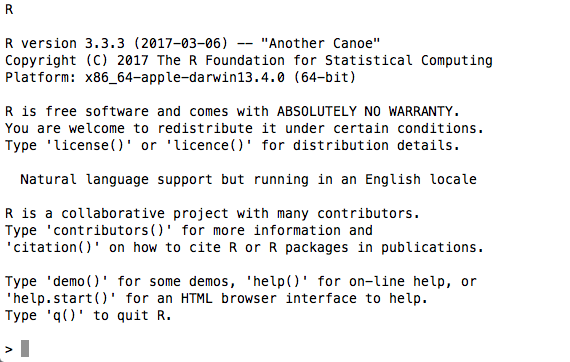
\includegraphics{images/rterminal.png}
\end{itemize}

\hypertarget{what-is-rstudio}{%
\chapter{What is RStudio ?}\label{what-is-rstudio}}

\begin{itemize}
\item
  Free and open source IDE (Integrated Development Environment) for R
\item
  Available for Windows, Mac OS and LINUX
\end{itemize}

\hypertarget{rstudio-access}{%
\section{RStudio access}\label{rstudio-access}}

\begin{itemize}
\item
  \href{https://www.rstudio.com/products/rstudio/download}{RStudio Desktop installation}
\item
  \href{http://rstudio.linux.crg.es/}{RStudio access from the CRG server}

  \begin{itemize}
  \tightlist
  \item
    Access with CRG credentials
  \item
    For those who don't have access to the CRG server, use the guest accounts.
  \end{itemize}
\end{itemize}

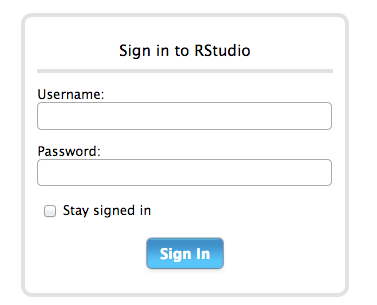
\includegraphics{images/rstudio_login.png}

\hypertarget{rstudio-interface}{%
\section{RStudio interface}\label{rstudio-interface}}

\begin{itemize}
\tightlist
\item
  4 panels:

  \begin{itemize}
  \tightlist
  \item
    top-left: scripts and files
  \item
    bottom-left: R terminal
  \item
    top-right: objects, history and environment
  \item
    bottom-right: tree of folders, graph window, packages, help window, viewer
  \end{itemize}
\end{itemize}

\hypertarget{setting-up-the-folder-structure-for-the-course}{%
\section{Setting up the folder structure for the course}\label{setting-up-the-folder-structure-for-the-course}}

Rcourse
\textbar{}-Module1
\textbar{}-Module2
\textbar{}-Module3
\textbar{}-Module4

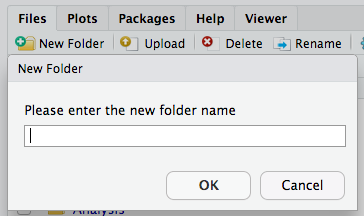
\includegraphics{images/rstudio_folder.png}

\hypertarget{paths-and-directories}{%
\chapter{Paths and directories}\label{paths-and-directories}}

\begin{itemize}
\item
  The path of a file/directory is its \textbf{location/address} in the file system.
\item
  Your home directory is the one that hosts your personal folder:

  \begin{itemize}
  \tightlist
  \item
    for CRG users: \textbf{/nfs/users/{[}yourgroup{]}/{[}yourusername{]}}
  \end{itemize}
\end{itemize}

\hypertarget{tree-of-directories}{%
\section{Tree of directories}\label{tree-of-directories}}

 \textasciitilde{}: shortcut to the home directory
 .: current directory
 ..: one directory up the tree

\hypertarget{navigate-the-tree-of-directory-with-the-r-terminal}{%
\section{Navigate the tree of directory with the R terminal}\label{navigate-the-tree-of-directory-with-the-r-terminal}}

\begin{itemize}
\tightlist
\item
  Get the path of the current directory (know where you are working at the moment) with getwd (get working directory):
\end{itemize}

\begin{Shaded}
\begin{Highlighting}[]
\KeywordTok{getwd}\NormalTok{()}
\end{Highlighting}
\end{Shaded}

\begin{itemize}
\tightlist
\item
  Change working directory with \textbf{setwd} (set working directory)
  Go to a directory giving the absolute path:
\end{itemize}

\begin{Shaded}
\begin{Highlighting}[]
\KeywordTok{setwd}\NormalTok{(}\StringTok{"~/Rcourse"}\NormalTok{)}
\end{Highlighting}
\end{Shaded}

Go to a directory giving the relative path:

\begin{Shaded}
\begin{Highlighting}[]
\KeywordTok{setwd}\NormalTok{(}\StringTok{"Module1"}\NormalTok{)}
\end{Highlighting}
\end{Shaded}

You are now in: ``\textasciitilde{}/Rcourse/Module1''
Move one directory ``up'' the tree:

\begin{Shaded}
\begin{Highlighting}[]
\KeywordTok{setwd}\NormalTok{(}\StringTok{".."}\NormalTok{)}
\end{Highlighting}
\end{Shaded}

You are now in: ``\textasciitilde{}/Rcourse''

\hypertarget{r-basics}{%
\chapter{R basics}\label{r-basics}}

\hypertarget{arithmetic-operators}{%
\section{Arithmetic operators}\label{arithmetic-operators}}

\begin{longtable}[]{@{}cc@{}}
\toprule
Operator & Function\tabularnewline
\midrule
\endhead
+ & addition\tabularnewline
- & subtraction\tabularnewline
/ & division\tabularnewline
* & multiplication\tabularnewline
\^{} or ** & exponential\tabularnewline
\bottomrule
\end{longtable}

In the R terminal:

\begin{Shaded}
\begin{Highlighting}[]
\DecValTok{10} \OperatorTok{-}\StringTok{ }\DecValTok{2}
\end{Highlighting}
\end{Shaded}

\begin{verbatim}
## [1] 8
\end{verbatim}

Type \textbf{Enter} for R to interpret the command.

\hypertarget{simple-calculations}{%
\section{Simple calculations}\label{simple-calculations}}

Given the following table:

\begin{longtable}[]{@{}cc@{}}
\toprule
type of RNA & Total\tabularnewline
\midrule
\endhead
mRNA & 329\tabularnewline
miRNA & 45\tabularnewline
snoRNA & 12\tabularnewline
lncRNA & 28\tabularnewline
\bottomrule
\end{longtable}

Calculate the total number of RNAs reported in the table:

\begin{Shaded}
\begin{Highlighting}[]
\DecValTok{329} \OperatorTok{+}\StringTok{ }\DecValTok{45} \OperatorTok{+}\StringTok{ }\DecValTok{12} \OperatorTok{+}\StringTok{ }\DecValTok{28}
\end{Highlighting}
\end{Shaded}

\begin{verbatim}
## [1] 414
\end{verbatim}

What is the percentage of miRNA?

\begin{Shaded}
\begin{Highlighting}[]
\NormalTok{( }\DecValTok{45} \OperatorTok{/}\StringTok{ }\DecValTok{414}\NormalTok{ ) }\OperatorTok{*}\StringTok{ }\DecValTok{100}
\end{Highlighting}
\end{Shaded}

\begin{verbatim}
## [1] 10.86957
\end{verbatim}

\hypertarget{objects-in-r}{%
\section{Objects in R}\label{objects-in-r}}

Everything that stores any kind of data in R is an \textbf{object}:

\#R syntax

\hypertarget{assignment-operators}{%
\section{Assignment operators}\label{assignment-operators}}

\begin{itemize}
\tightlist
\item
  \textbf{\textless{}-} or \textbf{=}
\item
  Essentially the same but, to avoid confusions:

  \begin{itemize}
  \tightlist
  \item
    Use \textbf{\textless{}-} for assignments
  \item
    Keep \textbf{=} for functions arguments
  \end{itemize}
\end{itemize}

\hypertarget{assigning-data-to-an-object}{%
\section{Assigning data to an object}\label{assigning-data-to-an-object}}

\begin{itemize}
\item
  Assigning a value to the object \textbf{B}:
  B \textless{}- 10
\item
  Reassigning: modifying the content of an object:
\end{itemize}

\begin{Shaded}
\begin{Highlighting}[]
\NormalTok{B }\OperatorTok{+}\StringTok{ }\DecValTok{10}
\end{Highlighting}
\end{Shaded}

{\textbf{B unchanged !!}}

\begin{Shaded}
\begin{Highlighting}[]
\NormalTok{B <-}\StringTok{ }\NormalTok{B }\OperatorTok{+}\StringTok{ }\DecValTok{10}
\end{Highlighting}
\end{Shaded}

{\textbf{B changed !!}}

\begin{itemize}
\tightlist
\item
  You can see the objects you created in the upper right panel in RStudio: the environment.
\end{itemize}

\hypertarget{functions}{%
\chapter{Functions}\label{functions}}

In programming, a function is a section of a program that \textbf{performs a specific task}.

For example, the function \textbf{getwd} is used as:

\begin{Shaded}
\begin{Highlighting}[]
\KeywordTok{getwd}\NormalTok{()}
\end{Highlighting}
\end{Shaded}

and has the task of outputting the current working directory.

You can recognize a function with the \textbf{round brackets}: function\textbf{()}

A function can also take \emph{arguments/parameters}

\begin{Shaded}
\begin{Highlighting}[]
\KeywordTok{setwd}\NormalTok{(}\DataTypeTok{dir=}\StringTok{"Rcourse"}\NormalTok{)}
\end{Highlighting}
\end{Shaded}

\textbf{setwd} changes the current working directory and takes one argument \textbf{dir}.

\begin{itemize}
\tightlist
\item
  Assign the output of a function to an object:
\end{itemize}

\begin{itemize}
\tightlist
\item
  Getting help: 
\end{itemize}

From the terminal:

\begin{Shaded}
\begin{Highlighting}[]
\KeywordTok{help}\NormalTok{(getwd)}
\NormalTok{?getwd}
\end{Highlighting}
\end{Shaded}

From the RStudio bottom-right panel:

\begin{itemize}
\tightlist
\item
  The help pages show:

  \begin{itemize}
  \tightlist
  \item
    required/optional argument(s), if any.
  \item
    default values for each argument(s), if any.
  \item
    examples.
  \item
    detailed description.
  \end{itemize}
\item
  Get the example of a function:
\end{itemize}

\begin{Shaded}
\begin{Highlighting}[]
\KeywordTok{example}\NormalTok{(mean)}
\end{Highlighting}
\end{Shaded}

\begin{verbatim}
## 
## mean> x <- c(0:10, 50)
## 
## mean> xm <- mean(x)
## 
## mean> c(xm, mean(x, trim = 0.10))
## [1] 8.75 5.50
\end{verbatim}

\begin{itemize}
\item
  Need more help? Ask your favourite \textbf{Web search engine !}
\item
  \textbf{Note on arguments}
\end{itemize}

The help page shows the compulsory arguments in the \textbf{Usage} section: in the help page of getwd and setwd (above), you can see that getwd doesn't take any compulsory argument, and setwd takes one compulsory argument that is called dir.
Compulsory arguments can be given \textbf{with their names}: in such case you don't need to respect a specific order, or \textbf{without their names}, in which case you have to respect the order specified in the help page!
For example, the \textbf{rep.int} function (a variant of the rep function) takes 2 arguments (see in help page): \textbf{x} and \textbf{times}, in that order:

\begin{Shaded}
\begin{Highlighting}[]
\CommentTok{# use arguments with their names:}
\KeywordTok{rep.int}\NormalTok{(}\DataTypeTok{x=}\DecValTok{1}\NormalTok{, }\DataTypeTok{times=}\DecValTok{3}\NormalTok{)}
\end{Highlighting}
\end{Shaded}

\begin{verbatim}
## [1] 1 1 1
\end{verbatim}

\begin{Shaded}
\begin{Highlighting}[]
\CommentTok{# use arguments with their names without respecting the order:}
\KeywordTok{rep.int}\NormalTok{(}\DataTypeTok{times=}\DecValTok{3}\NormalTok{, }\DataTypeTok{x=}\DecValTok{1}\NormalTok{)}
\end{Highlighting}
\end{Shaded}

\begin{verbatim}
## [1] 1 1 1
\end{verbatim}

\begin{Shaded}
\begin{Highlighting}[]
\CommentTok{# use arguments without their names but respecting the order:}
\KeywordTok{rep.int}\NormalTok{(}\DecValTok{1}\NormalTok{, }\DecValTok{3}\NormalTok{)}
\end{Highlighting}
\end{Shaded}

\begin{verbatim}
## [1] 1 1 1
\end{verbatim}

\begin{Shaded}
\begin{Highlighting}[]
\CommentTok{# use arguments without their names without respecting the order:}
\KeywordTok{rep.int}\NormalTok{(}\DecValTok{3}\NormalTok{, }\DecValTok{1}\NormalTok{)}
\end{Highlighting}
\end{Shaded}

\begin{verbatim}
## [1] 3
\end{verbatim}

\begin{Shaded}
\begin{Highlighting}[]
\CommentTok{# It works, but is not giving the expected output!}
\end{Highlighting}
\end{Shaded}

\hypertarget{r-scripts}{%
\chapter{R scripts}\label{r-scripts}}

\hypertarget{create-and-save-a-script}{%
\section{Create and save a script}\label{create-and-save-a-script}}

\begin{itemize}
\tightlist
\item
  Store commands in a .R/.r script. Create and save a script in RStudio with:

  \begin{itemize}
  \tightlist
  \item
    File -\textgreater{} New File -\textgreater{} R Script
  \item
    Once the file has opened: File -\textgreater{} Save
  \item
    Specify a name: \textbf{\emph{the extension .R is automatically added}}
  \end{itemize}
\item
  Execute commands or blocks of commands from RStudio:
\end{itemize}

\hypertarget{r-syntax}{%
\section{R syntax}\label{r-syntax}}

\begin{itemize}
\tightlist
\item
  Case sensitive: \textbf{g} is not \textbf{G}
\item
  Comment lines start with \textbf{\#}
\item
  Commands are separated by a \textbf{new line} or \textbf{;}
\end{itemize}

\begin{Shaded}
\begin{Highlighting}[]
\CommentTok{# This is a comment: it will not be interpreted}
\NormalTok{a <-}\StringTok{ }\DecValTok{10}
\NormalTok{A }\OperatorTok{+}\StringTok{ }\DecValTok{1}
\CommentTok{# Will throw an error because A and a are different}
\end{Highlighting}
\end{Shaded}

\hypertarget{rstudio-tips-in-the-console}{%
\section{RStudio tips in the console}\label{rstudio-tips-in-the-console}}

Ctrl + Enter: execute the current line.

 Upper arrow: goes to the commands previously typed.
Ctrl + cmd + : Browse command history.

 Type a letter in the console + ``tab'': R Studio proposes the different functions or object stored which start with that letter. for example, type \textbf{get + ``tab''}:

\hypertarget{exercice-1.-getting-started.}{%
\section{Exercice 1. Getting started.}\label{exercice-1.-getting-started.}}

Create the script ``exercise1.R'' (in R Studio: File -\textgreater{} New File) and save it to the ``Rcourse/Module1'' directory: you will save all the commands of exercise 1 in that script.
Remember you can comment the code using \#.

\textbf{1- From the terminal, go to Rcourse/Module1.
First check where you currently are with getwd();
then go to Rcourse/Module1 with setwd()}

correction

\begin{Shaded}
\begin{Highlighting}[]
\KeywordTok{getwd}\NormalTok{()}
\KeywordTok{setwd}\NormalTok{(}\StringTok{"Rcourse/Module1"}\NormalTok{)}
\KeywordTok{setwd}\NormalTok{(}\StringTok{"~/Rcourse/Module1"}\NormalTok{)}
\end{Highlighting}
\end{Shaded}

\textbf{2- Using R as a calculator, calculate the square root of 654.}

correction

\begin{Shaded}
\begin{Highlighting}[]
\KeywordTok{sqrt}\NormalTok{(}\DecValTok{654}\NormalTok{)}
\end{Highlighting}
\end{Shaded}

\begin{verbatim}
## [1] 25.57342
\end{verbatim}

\textbf{3- Using R as a calculator, calculate the percentage of males and females currently present in the classroom.}

correction

\begin{Shaded}
\begin{Highlighting}[]
\CommentTok{# 6 males out of 19 students:}
\NormalTok{(}\DecValTok{6}\OperatorTok{/}\DecValTok{19}\NormalTok{) }\OperatorTok{*}\StringTok{ }\DecValTok{100}
\end{Highlighting}
\end{Shaded}

\begin{verbatim}
## [1] 31.57895
\end{verbatim}

\begin{Shaded}
\begin{Highlighting}[]
\CommentTok{# 13 females out of 19 students}
\NormalTok{(}\DecValTok{13}\OperatorTok{/}\DecValTok{19}\NormalTok{) }\OperatorTok{*}\StringTok{ }\DecValTok{100}
\end{Highlighting}
\end{Shaded}

\begin{verbatim}
## [1] 68.42105
\end{verbatim}

\textbf{4- Create a new object ``myobject'' with value 60.
Show ``myobject'' in the terminal.}

correction

\begin{Shaded}
\begin{Highlighting}[]
\NormalTok{myobject <-}\StringTok{ }\DecValTok{60}
\NormalTok{myobject}
\end{Highlighting}
\end{Shaded}

\begin{verbatim}
## [1] 60
\end{verbatim}

\textbf{5- Reassign myobject with value 87.}

correction

\begin{Shaded}
\begin{Highlighting}[]
\NormalTok{myobject <-}\StringTok{ }\DecValTok{87}
\end{Highlighting}
\end{Shaded}

\textbf{6- Subtract 1 to myobject. Reassign.}

correction

\begin{Shaded}
\begin{Highlighting}[]
\NormalTok{myobject <-}\StringTok{ }\NormalTok{myobject }\OperatorTok{-}\StringTok{ }\DecValTok{1}
\end{Highlighting}
\end{Shaded}

\textbf{7- Create a new object ``mysqrt'' that will store the square root of ``myobject''.}

correction

\begin{Shaded}
\begin{Highlighting}[]
\NormalTok{mysqrt <-}\StringTok{ }\KeywordTok{sqrt}\NormalTok{(myobject)}
\end{Highlighting}
\end{Shaded}

\textbf{8- Create a new object ``mydiv'' that will store the result of ``myobject'' divided by ``mysqrt''.}

correction

\begin{Shaded}
\begin{Highlighting}[]
\NormalTok{mydiv <-}\StringTok{ }\NormalTok{myobject }\OperatorTok{/}\StringTok{ }\NormalTok{mysqrt}
\end{Highlighting}
\end{Shaded}

\hypertarget{data-types}{%
\chapter{Data types}\label{data-types}}

Each object has a data type:
* Numeric (number - integer or double)
* Character (text)
* Logical (TRUE / FALSE)

\#\#Checking data types

Number:

\begin{Shaded}
\begin{Highlighting}[]
\NormalTok{a <-}\StringTok{ }\DecValTok{10}
\KeywordTok{mode}\NormalTok{(a)}
\end{Highlighting}
\end{Shaded}

\begin{verbatim}
## [1] "numeric"
\end{verbatim}

\begin{Shaded}
\begin{Highlighting}[]
\KeywordTok{typeof}\NormalTok{(a)}
\end{Highlighting}
\end{Shaded}

\begin{verbatim}
## [1] "double"
\end{verbatim}

\begin{Shaded}
\begin{Highlighting}[]
\KeywordTok{str}\NormalTok{(a)}
\end{Highlighting}
\end{Shaded}

\begin{verbatim}
##  num 10
\end{verbatim}

Text:

\begin{Shaded}
\begin{Highlighting}[]
\NormalTok{b <-}\StringTok{ "word"}
\KeywordTok{mode}\NormalTok{(b)}
\end{Highlighting}
\end{Shaded}

\begin{verbatim}
## [1] "character"
\end{verbatim}

\begin{Shaded}
\begin{Highlighting}[]
\KeywordTok{typeof}\NormalTok{(b)}
\end{Highlighting}
\end{Shaded}

\begin{verbatim}
## [1] "character"
\end{verbatim}

\begin{Shaded}
\begin{Highlighting}[]
\KeywordTok{str}\NormalTok{(b)}
\end{Highlighting}
\end{Shaded}

\begin{verbatim}
##  chr "word"
\end{verbatim}

\hypertarget{data-structures}{%
\chapter{Data structures}\label{data-structures}}

The main data structures are:

\begin{itemize}
\tightlist
\item
  Vector
\item
  Factor
\item
  Matrix
\item
  Data frame
\end{itemize}

\hypertarget{vectors}{%
\section{Vectors}\label{vectors}}

A vector is a sequence of data elements from the \textbf{same type}.

329 \textbar{} 45 \textbar{} 12 \textbar{} 28 \textbar{}

\hypertarget{creating-a-vector}{%
\subsection{Creating a vector}\label{creating-a-vector}}

\begin{itemize}
\tightlist
\item
  Values are assigned to a vector using the \textbf{c} command (\textbf{c}ombining elements).
\end{itemize}

\begin{Shaded}
\begin{Highlighting}[]
\NormalTok{a <-}\StringTok{ }\KeywordTok{c}\NormalTok{(}\DecValTok{329}\NormalTok{, }\DecValTok{45}\NormalTok{, }\DecValTok{12}\NormalTok{, }\DecValTok{28}\NormalTok{)}
\end{Highlighting}
\end{Shaded}

You can create an empty vector with:

\begin{Shaded}
\begin{Highlighting}[]
\NormalTok{vecempty <-}\StringTok{ }\KeywordTok{vector}\NormalTok{()}
\end{Highlighting}
\end{Shaded}

\begin{itemize}
\tightlist
\item
  Create a sequence of consecutive numbers:
\end{itemize}

\begin{Shaded}
\begin{Highlighting}[]
\NormalTok{a <-}\StringTok{ }\DecValTok{1}\OperatorTok{:}\DecValTok{6}
\CommentTok{# same as:}
\NormalTok{a <-}\StringTok{ }\KeywordTok{c}\NormalTok{(}\DecValTok{1}\NormalTok{, }\DecValTok{2}\NormalTok{, }\DecValTok{3}\NormalTok{, }\DecValTok{4}\NormalTok{, }\DecValTok{5}\NormalTok{, }\DecValTok{6}\NormalTok{)}
\CommentTok{# both ends (1 and 6) are included}
\end{Highlighting}
\end{Shaded}

\begin{itemize}
\tightlist
\item
  Character vectors: Each element is entered between (single or double) quotes.
\end{itemize}

mRNA \textbar{} miRNA \textbar{} snoRNA \textbar{} lncRNA \textbar{}

\begin{Shaded}
\begin{Highlighting}[]
\NormalTok{b <-}\StringTok{ }\KeywordTok{c}\NormalTok{(}\StringTok{"mRNA"}\NormalTok{, }\StringTok{"miRNA"}\NormalTok{, }\StringTok{"snoRNA"}\NormalTok{, }\StringTok{"lncRNA"}\NormalTok{)}
\end{Highlighting}
\end{Shaded}

\hypertarget{vector-manipulation}{%
\subsection{Vector manipulation}\label{vector-manipulation}}

\begin{itemize}
\tightlist
\item
  A vector can be \textbf{named}: each element of the vector can be assigned a name (number or character)
\end{itemize}

\begin{Shaded}
\begin{Highlighting}[]
\KeywordTok{names}\NormalTok{(a) <-}\StringTok{ }\KeywordTok{c}\NormalTok{(}\StringTok{"mRNA"}\NormalTok{, }\StringTok{"miRNA"}\NormalTok{, }\StringTok{"snoRNA"}\NormalTok{, }\StringTok{"lncRNA"}\NormalTok{)}
\CommentTok{# use an object which already contains a vector}
\KeywordTok{names}\NormalTok{(a) <-}\StringTok{ }\NormalTok{b}
\end{Highlighting}
\end{Shaded}

\begin{itemize}
\tightlist
\item
  Get the length (number of elements) of a vector
\end{itemize}

\begin{Shaded}
\begin{Highlighting}[]
\KeywordTok{length}\NormalTok{(a)}
\end{Highlighting}
\end{Shaded}

\begin{verbatim}
## [1] 6
\end{verbatim}

\begin{itemize}
\tightlist
\item
  Extracting elements from vector \textbf{a}

  \begin{itemize}
  \tightlist
  \item
    extract elements using their position (index) in the vector:
  \end{itemize}

\begin{Shaded}
\begin{Highlighting}[]
\NormalTok{a <-}\StringTok{ }\DecValTok{1}\OperatorTok{:}\DecValTok{6}
\NormalTok{a[}\DecValTok{1}\NormalTok{]}
\end{Highlighting}
\end{Shaded}

\begin{verbatim}
## [1] 1
\end{verbatim}

\begin{Shaded}
\begin{Highlighting}[]
\NormalTok{a[}\KeywordTok{c}\NormalTok{(}\DecValTok{1}\NormalTok{,}\DecValTok{3}\NormalTok{)]}
\end{Highlighting}
\end{Shaded}

\begin{verbatim}
## [1] 1 3
\end{verbatim}

\begin{Shaded}
\begin{Highlighting}[]
\NormalTok{a[}\DecValTok{2}\OperatorTok{:}\DecValTok{4}\NormalTok{]}
\end{Highlighting}
\end{Shaded}

\begin{verbatim}
## [1] 2 3 4
\end{verbatim}

  \begin{itemize}
  \tightlist
  \item
    extract elements using their names:
  \end{itemize}

\begin{Shaded}
\begin{Highlighting}[]
\NormalTok{a[}\StringTok{"mRNA"}\NormalTok{]}
\end{Highlighting}
\end{Shaded}

\begin{verbatim}
## [1] NA
\end{verbatim}

\begin{Shaded}
\begin{Highlighting}[]
\NormalTok{a[}\KeywordTok{c}\NormalTok{(}\StringTok{"miRNA"}\NormalTok{, }\StringTok{"lncRNA"}\NormalTok{)]            }
\end{Highlighting}
\end{Shaded}

\begin{verbatim}
## [1] NA NA
\end{verbatim}
\item
  Reassigning a vector's element
\end{itemize}

\begin{Shaded}
\begin{Highlighting}[]
\NormalTok{a[}\DecValTok{2}\NormalTok{] <-}\StringTok{ }\DecValTok{31}
\NormalTok{a[}\StringTok{"miRNA"}\NormalTok{] <-}\StringTok{ }\DecValTok{31}
\end{Highlighting}
\end{Shaded}

\begin{itemize}
\tightlist
\item
  Removing a vector's element
\end{itemize}

\begin{Shaded}
\begin{Highlighting}[]
\NormalTok{a <-}\StringTok{ }\NormalTok{a[}\OperatorTok{-}\DecValTok{3}\NormalTok{]}
\end{Highlighting}
\end{Shaded}

\begin{itemize}
\tightlist
\item
  \textbf{Show} versus \textbf{change}
\end{itemize}

x{[}-2{]} x {unchanged} !

x \textless{}- x{[}-2{]} x {reassigned} !

\hypertarget{combining-vectors}{%
\subsection{Combining vectors}\label{combining-vectors}}

\begin{itemize}
\tightlist
\item
  From 2 vectors \textbf{a} and \textbf{b} you can create a vector \textbf{d}
\end{itemize}

\begin{Shaded}
\begin{Highlighting}[]
\NormalTok{a <-}\StringTok{ }\DecValTok{2}\OperatorTok{:}\DecValTok{5}
\NormalTok{b <-}\StringTok{ }\DecValTok{4}\OperatorTok{:}\DecValTok{6}
\NormalTok{d <-}\StringTok{ }\KeywordTok{c}\NormalTok{(a, b)}
\end{Highlighting}
\end{Shaded}

\begin{quote}
The elements of \textbf{b} are added after the elements of \textbf{a}
\end{quote}

\begin{itemize}
\tightlist
\item
  Likewise, you can add elements at the end of a vector
\end{itemize}

\begin{Shaded}
\begin{Highlighting}[]
\NormalTok{d <-}\StringTok{ }\KeywordTok{c}\NormalTok{(d, }\DecValTok{19}\NormalTok{)}
\end{Highlighting}
\end{Shaded}

\hypertarget{numeric-vector-manipulation}{%
\subsection{Numeric vector manipulation}\label{numeric-vector-manipulation}}

Logical operators

\begin{longtable}[]{@{}cc@{}}
\toprule
Operator & Description\tabularnewline
\midrule
\endhead
\textless{} & less than\tabularnewline
\textless{}= & less than or equal to\tabularnewline
\textgreater{} & greater than\tabularnewline
\textgreater{}= & greater than or equal to\tabularnewline
== & exactly equal to\tabularnewline
!= & not equal to\tabularnewline
!x & not x\tabularnewline
x \textbar{} y & x OR y\tabularnewline
x \& y & x AND y\tabularnewline
\bottomrule
\end{longtable}

\begin{itemize}
\tightlist
\item
  Which elements of \textbf{a} are equal to 2?
\end{itemize}

\begin{Shaded}
\begin{Highlighting}[]
\NormalTok{a <-}\StringTok{ }\DecValTok{1}\OperatorTok{:}\DecValTok{5}
\NormalTok{a }\OperatorTok{==}\StringTok{ }\DecValTok{2}
\end{Highlighting}
\end{Shaded}

\begin{verbatim}
## [1] FALSE  TRUE FALSE FALSE FALSE
\end{verbatim}

\begin{itemize}
\tightlist
\item
  Which elements of \textbf{a} are superior to 2?
\end{itemize}

\begin{Shaded}
\begin{Highlighting}[]
\NormalTok{a <-}\StringTok{ }\DecValTok{1}\OperatorTok{:}\DecValTok{5}
\NormalTok{a }\OperatorTok{>}\StringTok{ }\DecValTok{2}
\end{Highlighting}
\end{Shaded}

\begin{verbatim}
## [1] FALSE FALSE  TRUE  TRUE  TRUE
\end{verbatim}

\begin{itemize}
\tightlist
\item
  Extract elements of a vector that comply with a condition:
\end{itemize}

\begin{Shaded}
\begin{Highlighting}[]
\NormalTok{a <-}\StringTok{ }\DecValTok{1}\OperatorTok{:}\DecValTok{5}
\NormalTok{a }\OperatorTok{>=}\StringTok{ }\DecValTok{2}
\end{Highlighting}
\end{Shaded}

\begin{verbatim}
## [1] FALSE  TRUE  TRUE  TRUE  TRUE
\end{verbatim}

\begin{Shaded}
\begin{Highlighting}[]
\NormalTok{a[a }\OperatorTok{>=}\StringTok{ }\DecValTok{2}\NormalTok{]}
\end{Highlighting}
\end{Shaded}

\begin{verbatim}
## [1] 2 3 4 5
\end{verbatim}

\hypertarget{operations-on-vectors}{%
\subsubsection{Operations on vectors}\label{operations-on-vectors}}

\begin{itemize}
\tightlist
\item
  Adding 2 to a vector adds 2 to \textbf{each element} of the vector:
\end{itemize}

\begin{Shaded}
\begin{Highlighting}[]
\NormalTok{a <-}\StringTok{ }\DecValTok{1}\OperatorTok{:}\DecValTok{5}
\NormalTok{a }\OperatorTok{+}\StringTok{ }\DecValTok{2}
\end{Highlighting}
\end{Shaded}

\begin{verbatim}
## [1] 3 4 5 6 7
\end{verbatim}

\begin{quote}
Same goes for subtractions, multiplications and divisions\ldots{}
\end{quote}

\begin{itemize}
\tightlist
\item
  Multiplying a vector by another vector of equal length
\end{itemize}

\begin{Shaded}
\begin{Highlighting}[]
\NormalTok{a <-}\StringTok{ }\KeywordTok{c}\NormalTok{(}\DecValTok{2}\NormalTok{, }\DecValTok{4}\NormalTok{, }\DecValTok{6}\NormalTok{)}
\NormalTok{b <-}\StringTok{ }\KeywordTok{c}\NormalTok{(}\DecValTok{2}\NormalTok{, }\DecValTok{3}\NormalTok{, }\DecValTok{0}\NormalTok{)}
\NormalTok{a }\OperatorTok{*}\StringTok{ }\NormalTok{b}
\end{Highlighting}
\end{Shaded}

\begin{verbatim}
## [1]  4 12  0
\end{verbatim}

\begin{itemize}
\tightlist
\item
  Multiplying a vector by another \textbf{shorter} vector
\end{itemize}

\begin{Shaded}
\begin{Highlighting}[]
\NormalTok{a <-}\StringTok{ }\KeywordTok{c}\NormalTok{(}\DecValTok{2}\NormalTok{, }\DecValTok{4}\NormalTok{, }\DecValTok{6}\NormalTok{, }\DecValTok{3}\NormalTok{, }\DecValTok{1}\NormalTok{)}
\NormalTok{b <-}\StringTok{ }\KeywordTok{c}\NormalTok{(}\DecValTok{2}\NormalTok{, }\DecValTok{3}\NormalTok{, }\DecValTok{0}\NormalTok{)}
\NormalTok{a }\OperatorTok{*}\StringTok{ }\NormalTok{b}
\end{Highlighting}
\end{Shaded}

\begin{verbatim}
## Warning in a * b: longer object length is not a multiple of shorter object
## length
\end{verbatim}

\begin{verbatim}
## [1]  4 12  0  6  3
\end{verbatim}

\begin{quote}
Vector \textbf{a} is ``recycled'' !
\end{quote}

\begin{itemize}
\tightlist
\item
  Summary statistics
\end{itemize}

\begin{longtable}[]{@{}cc@{}}
\toprule
Function & Description\tabularnewline
\midrule
\endhead
mean(x) & mean / average\tabularnewline
median(x) & median\tabularnewline
min(x) & minimum\tabularnewline
max(x) & maximum\tabularnewline
var(x) & variance\tabularnewline
summary(x) & mean, median, min, max, quartiles\tabularnewline
\bottomrule
\end{longtable}

\begin{Shaded}
\begin{Highlighting}[]
\NormalTok{a <-}\StringTok{ }\KeywordTok{c}\NormalTok{(}\DecValTok{1}\NormalTok{, }\DecValTok{3}\NormalTok{, }\DecValTok{12}\NormalTok{, }\DecValTok{45}\NormalTok{, }\DecValTok{3}\NormalTok{, }\DecValTok{2}\NormalTok{)}
\KeywordTok{summary}\NormalTok{(a)}
\end{Highlighting}
\end{Shaded}

\begin{verbatim}
##    Min. 1st Qu.  Median    Mean 3rd Qu.    Max. 
##    1.00    2.25    3.00   11.00    9.75   45.00
\end{verbatim}

\hypertarget{comparing-vectors}{%
\subsubsection{Comparing vectors}\label{comparing-vectors}}

\begin{itemize}
\tightlist
\item
  The \textbf{\%in\%} operator
\end{itemize}

Which elements of \textbf{a} are also found in **b* ?

\begin{Shaded}
\begin{Highlighting}[]
\NormalTok{a <-}\StringTok{ }\DecValTok{2}\OperatorTok{:}\DecValTok{6}
\NormalTok{b <-}\StringTok{ }\DecValTok{4}\OperatorTok{:}\DecValTok{10}
\NormalTok{a }\OperatorTok\StringTok{ }\NormalTok{b}
\end{Highlighting}
\end{Shaded}

\begin{verbatim}
## [1] FALSE FALSE  TRUE  TRUE  TRUE
\end{verbatim}

Retrieve actual elements of \textbf{a} that are found in \textbf{b}:

\begin{Shaded}
\begin{Highlighting}[]
\NormalTok{a <-}\StringTok{ }\DecValTok{2}\OperatorTok{:}\DecValTok{6}
\NormalTok{b <-}\StringTok{ }\DecValTok{4}\OperatorTok{:}\DecValTok{10}
\NormalTok{a[a }\OperatorTok\StringTok{ }\NormalTok{b]}
\end{Highlighting}
\end{Shaded}

\begin{verbatim}
## [1] 4 5 6
\end{verbatim}

\hypertarget{character-vector-manipulation}{%
\subsection{Character vector manipulation}\label{character-vector-manipulation}}

Character vectors are manipulated similarly to numeric ones.

\begin{itemize}
\tightlist
\item
  The \textbf{\%in\%} operator:
\end{itemize}

\begin{Shaded}
\begin{Highlighting}[]
\NormalTok{k <-}\StringTok{ }\KeywordTok{c}\NormalTok{(}\StringTok{"mRNA"}\NormalTok{, }\StringTok{"miRNA"}\NormalTok{, }\StringTok{"snoRNA"}\NormalTok{, }\StringTok{"RNA"}\NormalTok{, }\StringTok{"lincRNA"}\NormalTok{)}
\NormalTok{p <-}\StringTok{ }\KeywordTok{c}\NormalTok{(}\StringTok{"mRNA"}\NormalTok{,}\StringTok{"lincRNA"}\NormalTok{, }\StringTok{"tRNA"}\NormalTok{, }\StringTok{"miRNA"}\NormalTok{)}
\NormalTok{k }\OperatorTok\StringTok{ }\NormalTok{p}
\end{Highlighting}
\end{Shaded}

\begin{verbatim}
## [1]  TRUE  TRUE FALSE FALSE  TRUE
\end{verbatim}

\begin{Shaded}
\begin{Highlighting}[]
\NormalTok{k[k }\OperatorTok\StringTok{ }\NormalTok{p]}
\end{Highlighting}
\end{Shaded}

\begin{verbatim}
## [1] "mRNA"    "miRNA"   "lincRNA"
\end{verbatim}

\begin{itemize}
\tightlist
\item
  Select elements from vector \textbf{m} that are not \emph{exon}
\end{itemize}

\begin{Shaded}
\begin{Highlighting}[]
\NormalTok{m <-}\StringTok{ }\KeywordTok{c}\NormalTok{(}\StringTok{"exon"}\NormalTok{, }\StringTok{"intron"}\NormalTok{, }\StringTok{"exon"}\NormalTok{)}
\NormalTok{m }\OperatorTok{!=}\StringTok{ "exon"}
\end{Highlighting}
\end{Shaded}

\begin{verbatim}
## [1] FALSE  TRUE FALSE
\end{verbatim}

\begin{Shaded}
\begin{Highlighting}[]
\NormalTok{m[m }\OperatorTok{!=}\StringTok{ "exon"}\NormalTok{]}
\end{Highlighting}
\end{Shaded}

\begin{verbatim}
## [1] "intron"
\end{verbatim}

\hypertarget{exercise-2.-numeric-vector-manipulation}{%
\section{Exercise 2. Numeric vector manipulation}\label{exercise-2.-numeric-vector-manipulation}}

\hypertarget{exercise-2a.}{%
\subsection{Exercise 2a.}\label{exercise-2a.}}

Create the script ``exercise2.R'' and save it to the ``Rcourse/Module1'' directory: you will save all the commands of exercise 2 in that script.
Remember you can comment the code using \#.

\textbf{1- Go to Rcourse/Module1
First check where you currently are with getwd();
then go to Rcourse/Module1 with setwd()}

correction

\begin{Shaded}
\begin{Highlighting}[]
\KeywordTok{getwd}\NormalTok{()}
\KeywordTok{setwd}\NormalTok{(}\StringTok{"Rcourse/Module1"}\NormalTok{)}
\KeywordTok{setwd}\NormalTok{(}\StringTok{"~/Rcourse/Module1"}\NormalTok{)}
\end{Highlighting}
\end{Shaded}

\textbf{2- Create a numeric vector y which contains the numbers from 2 to 11, both included.}
Show y in the terminal.

correction

\begin{Shaded}
\begin{Highlighting}[]
\NormalTok{y <-}\StringTok{ }\KeywordTok{c}\NormalTok{(}\DecValTok{2}\NormalTok{, }\DecValTok{3}\NormalTok{, }\DecValTok{4}\NormalTok{, }\DecValTok{5}\NormalTok{, }\DecValTok{6}\NormalTok{, }\DecValTok{7}\NormalTok{, }\DecValTok{8}\NormalTok{, }\DecValTok{9}\NormalTok{, }\DecValTok{10}\NormalTok{, }\DecValTok{11}\NormalTok{)}
\CommentTok{# same as}
\NormalTok{y <-}\StringTok{ }\DecValTok{2}\OperatorTok{:}\DecValTok{11}
\CommentTok{# show in terminal:}
\NormalTok{y}
\end{Highlighting}
\end{Shaded}

\begin{verbatim}
##  [1]  2  3  4  5  6  7  8  9 10 11
\end{verbatim}

\textbf{3- How many elements are in y? I.e what is the length of vector y ?}

correction

\begin{Shaded}
\begin{Highlighting}[]
\KeywordTok{length}\NormalTok{(y)}
\end{Highlighting}
\end{Shaded}

\begin{verbatim}
## [1] 10
\end{verbatim}

\textbf{4- Show the 2nd element of y.}

correction

\begin{Shaded}
\begin{Highlighting}[]
\NormalTok{y[}\DecValTok{2}\NormalTok{]}
\end{Highlighting}
\end{Shaded}

\begin{verbatim}
## [1] 3
\end{verbatim}

\textbf{5- Show the 3rd and the 6th elements of y.}

correction

\begin{Shaded}
\begin{Highlighting}[]
\NormalTok{y[}\KeywordTok{c}\NormalTok{(}\DecValTok{3}\NormalTok{,}\DecValTok{6}\NormalTok{)]}
\end{Highlighting}
\end{Shaded}

\begin{verbatim}
## [1] 4 7
\end{verbatim}

\textbf{6- Remove the 4th element of y: reassign. What is now the length of y ?}

correction

\begin{Shaded}
\begin{Highlighting}[]
\CommentTok{# remove 4th element and reassign}
\NormalTok{y <-}\StringTok{ }\NormalTok{y[}\OperatorTok{-}\DecValTok{4}\NormalTok{]}
\CommentTok{# length of y}
\KeywordTok{length}\NormalTok{(y)}
\end{Highlighting}
\end{Shaded}

\begin{verbatim}
## [1] 9
\end{verbatim}

\textbf{7- Show all elements of y that are less than 7.}

correction

\begin{Shaded}
\begin{Highlighting}[]
\CommentTok{# which elements of y are less than 7:}
\NormalTok{y }\OperatorTok{<}\StringTok{ }\DecValTok{7}
\end{Highlighting}
\end{Shaded}

\begin{verbatim}
## [1]  TRUE  TRUE  TRUE  TRUE FALSE FALSE FALSE FALSE FALSE
\end{verbatim}

\begin{Shaded}
\begin{Highlighting}[]
\CommentTok{# show those elements }
\NormalTok{y[ y }\OperatorTok{<}\StringTok{ }\DecValTok{7}\NormalTok{ ]}
\end{Highlighting}
\end{Shaded}

\begin{verbatim}
## [1] 2 3 4 6
\end{verbatim}

\textbf{8- Show all elements of y that are greater or equal to 4 and less than 9.}

correction

\begin{Shaded}
\begin{Highlighting}[]
\NormalTok{y[ y }\OperatorTok{>=}\StringTok{ }\DecValTok{4} \OperatorTok{&}\StringTok{ }\NormalTok{y }\OperatorTok{<}\StringTok{ }\DecValTok{9}\NormalTok{ ]}
\end{Highlighting}
\end{Shaded}

\begin{verbatim}
## [1] 4 6 7 8
\end{verbatim}

\textbf{9- Create the vector x of 1000 random numbers from the normal distribution:}
\textbf{\emph{First read the help page of the rnorm() function.}}

correction

\begin{Shaded}
\begin{Highlighting}[]
\CommentTok{# help page for the rnorm function}
\KeywordTok{help}\NormalTok{(rnorm)}
\CommentTok{# produce a vector of 1000 random numbers from the normal distribution}
\NormalTok{x <-}\StringTok{ }\KeywordTok{rnorm}\NormalTok{(}\DecValTok{1000}\NormalTok{)}
\end{Highlighting}
\end{Shaded}

\textbf{10. What are the mean, median, minimum and maximum values of x?}

correction

\begin{Shaded}
\begin{Highlighting}[]
\KeywordTok{mean}\NormalTok{(x); }\KeywordTok{median}\NormalTok{(x); }\KeywordTok{min}\NormalTok{(x); }\KeywordTok{max}\NormalTok{(x)}
\end{Highlighting}
\end{Shaded}

\begin{verbatim}
## [1] -0.0024426
\end{verbatim}

\begin{verbatim}
## [1] -0.01987436
\end{verbatim}

\begin{verbatim}
## [1] -4.276704
\end{verbatim}

\begin{verbatim}
## [1] 3.721429
\end{verbatim}

\textbf{11- Run the summary() function on x. What additional information do you obtain ?}

correction

\begin{Shaded}
\begin{Highlighting}[]
\KeywordTok{summary}\NormalTok{(x)}
\end{Highlighting}
\end{Shaded}

\begin{verbatim}
##      Min.   1st Qu.    Median      Mean   3rd Qu.      Max. 
## -4.277000 -0.689500 -0.019870 -0.002443  0.625900  3.721000
\end{verbatim}

\textbf{12- Create vector y2 as:}

\begin{Shaded}
\begin{Highlighting}[]
\NormalTok{y2 <-}\StringTok{ }\KeywordTok{c}\NormalTok{(}\DecValTok{1}\NormalTok{, }\DecValTok{11}\NormalTok{, }\DecValTok{5}\NormalTok{, }\DecValTok{62}\NormalTok{,  }\DecValTok{18}\NormalTok{, }\DecValTok{2}\NormalTok{, }\DecValTok{8}\NormalTok{)}
\end{Highlighting}
\end{Shaded}

\textbf{13. What is the sum of all elements in y2 ?}

correction

\begin{Shaded}
\begin{Highlighting}[]
\KeywordTok{sum}\NormalTok{(y2)}
\end{Highlighting}
\end{Shaded}

\begin{verbatim}
## [1] 107
\end{verbatim}

\textbf{14- Which elements of y2 are also present in y ?
Note: remember the \%in\% operator.}

correction

\begin{Shaded}
\begin{Highlighting}[]
\NormalTok{y2[ y2 }\OperatorTok\StringTok{ }\NormalTok{y ]}
\end{Highlighting}
\end{Shaded}

\begin{verbatim}
## [1] 11  2  8
\end{verbatim}

\textbf{15- Multiply each element of y2 by 1.5: reassign.}

correction

\begin{Shaded}
\begin{Highlighting}[]
\NormalTok{y2 <-}\StringTok{ }\NormalTok{y2 }\OperatorTok{*}\StringTok{ }\FloatTok{1.5}
\end{Highlighting}
\end{Shaded}

\textbf{16- Use the function any() to check if the number 3 is present.}

correction

\begin{Shaded}
\begin{Highlighting}[]
\CommentTok{# "Given a set of logical vectors, is at least one of the values true?"}
\KeywordTok{any}\NormalTok{( y2 }\OperatorTok{==}\StringTok{ }\DecValTok{3}\NormalTok{ )}
\end{Highlighting}
\end{Shaded}

\begin{verbatim}
## [1] TRUE
\end{verbatim}

\hypertarget{exercise-2b.}{%
\subsection{Exercise 2b.}\label{exercise-2b.}}

\textbf{1- Create the vector myvector as:}

\begin{Shaded}
\begin{Highlighting}[]
\NormalTok{myvector <-}\StringTok{ }\KeywordTok{c}\NormalTok{(}\DecValTok{1}\NormalTok{, }\DecValTok{2}\NormalTok{, }\DecValTok{3}\NormalTok{, }\DecValTok{1}\NormalTok{, }\DecValTok{2}\NormalTok{, }\DecValTok{3}\NormalTok{, }\DecValTok{1}\NormalTok{, }\DecValTok{2}\NormalTok{, }\DecValTok{3}\NormalTok{)}
\end{Highlighting}
\end{Shaded}

\textbf{Create the same vector using the rep() function (?rep)}

correction

\begin{Shaded}
\begin{Highlighting}[]
\NormalTok{myvector <-}\StringTok{ }\KeywordTok{rep}\NormalTok{(}\DecValTok{1}\OperatorTok{:}\DecValTok{3}\NormalTok{, }\DecValTok{3}\NormalTok{)}
\end{Highlighting}
\end{Shaded}

\textbf{2- Reassign the 5th, 6th and 7th position of myvector with the values 8, 12 and 32, respectively.}

correction

\begin{Shaded}
\begin{Highlighting}[]
\CommentTok{# reassign one by one}
\NormalTok{myvector[}\DecValTok{5}\NormalTok{] <-}\StringTok{ }\DecValTok{8}
\NormalTok{myvector[}\DecValTok{6}\NormalTok{] <-}\StringTok{ }\DecValTok{12}
\NormalTok{myvector[}\DecValTok{7}\NormalTok{] <-}\StringTok{ }\DecValTok{32}
\CommentTok{# or reassign all at once}
\NormalTok{myvector[}\DecValTok{5}\OperatorTok{:}\DecValTok{7}\NormalTok{] <-}\StringTok{ }\KeywordTok{c}\NormalTok{(}\DecValTok{8}\NormalTok{, }\DecValTok{12}\NormalTok{, }\DecValTok{32}\NormalTok{)}
\end{Highlighting}
\end{Shaded}

\textbf{3- Calculate the fraction/percentage of each element of myvector (relative to the sum of all elements of the vector).
sum() can be useful.}

correction

\begin{Shaded}
\begin{Highlighting}[]
\CommentTok{# sum of all elements of the vector}
\NormalTok{mytotal <-}\StringTok{ }\KeywordTok{sum}\NormalTok{(myvector)}
\CommentTok{# divide each element by the sum}
\NormalTok{myvector }\OperatorTok{/}\StringTok{ }\NormalTok{mytotal}
\end{Highlighting}
\end{Shaded}

\begin{verbatim}
## [1] 0.015625 0.031250 0.046875 0.015625 0.125000 0.187500 0.500000 0.031250
## [9] 0.046875
\end{verbatim}

\begin{Shaded}
\begin{Highlighting}[]
\CommentTok{# multiply by 100 to get a percentage}
\NormalTok{(myvector }\OperatorTok{/}\StringTok{ }\NormalTok{mytotal) }\OperatorTok{*}\StringTok{ }\DecValTok{100}
\end{Highlighting}
\end{Shaded}

\begin{verbatim}
## [1]  1.5625  3.1250  4.6875  1.5625 12.5000 18.7500 50.0000  3.1250  4.6875
\end{verbatim}

\textbf{4- Add vector c(2, 4, 6, 7) to myvector (combining both vectors): reassign!}

correction

\begin{Shaded}
\begin{Highlighting}[]
\CommentTok{# create the new vector}
\NormalTok{newvector <-}\StringTok{ }\KeywordTok{c}\NormalTok{(}\DecValTok{2}\NormalTok{, }\DecValTok{4}\NormalTok{, }\DecValTok{6}\NormalTok{, }\DecValTok{7}\NormalTok{)}
\CommentTok{# combine both myvector and newvector}
\KeywordTok{c}\NormalTok{(myvector, newvector)}
\end{Highlighting}
\end{Shaded}

\begin{verbatim}
##  [1]  1  2  3  1  8 12 32  2  3  2  4  6  7
\end{verbatim}

\begin{Shaded}
\begin{Highlighting}[]
\CommentTok{# reassign myvector}
\NormalTok{myvector <-}\StringTok{ }\KeywordTok{c}\NormalTok{(myvector, newvector)}
\end{Highlighting}
\end{Shaded}

\hypertarget{exercise-3.-character-vector-manipulation}{%
\section{Exercise 3. Character vector manipulation}\label{exercise-3.-character-vector-manipulation}}

\hypertarget{exercise-3a.}{%
\subsection{Exercise 3a.}\label{exercise-3a.}}

Create the script ``exercise3.R'' and save it to the ``Rcourse/Module1'' directory: you will save all the commands of exercise 3 in that script.
Remember you can comment the code using \#.

\textbf{1- Go to Rcourse/Module1
First check where you currently are with getwd();
then go to Rcourse/Module1 with setwd()}

correction

\begin{Shaded}
\begin{Highlighting}[]
\KeywordTok{getwd}\NormalTok{()}
\KeywordTok{setwd}\NormalTok{(}\StringTok{"Rcourse/Module1"}\NormalTok{)}
\KeywordTok{setwd}\NormalTok{(}\StringTok{"~/Rcourse/Module1"}\NormalTok{)}
\end{Highlighting}
\end{Shaded}

\textbf{2- Create vector w as:}

\begin{Shaded}
\begin{Highlighting}[]
\NormalTok{w <-}\StringTok{ }\KeywordTok{rep}\NormalTok{(}\DataTypeTok{x=}\KeywordTok{c}\NormalTok{(}\StringTok{"miRNA"}\NormalTok{, }\StringTok{"mRNA"}\NormalTok{), }\DataTypeTok{times=}\KeywordTok{c}\NormalTok{(}\DecValTok{3}\NormalTok{, }\DecValTok{2}\NormalTok{))}
\end{Highlighting}
\end{Shaded}

\textbf{3- View vector w in the console: how does function rep() work ?}
Play with the \textbf{times} argument.

correction

\begin{Shaded}
\begin{Highlighting}[]
\KeywordTok{rep}\NormalTok{(}\DataTypeTok{x=}\KeywordTok{c}\NormalTok{(}\StringTok{"miRNA"}\NormalTok{, }\StringTok{"mRNA"}\NormalTok{), }\DataTypeTok{times=}\KeywordTok{c}\NormalTok{(}\DecValTok{3}\NormalTok{, }\DecValTok{4}\NormalTok{))}
\end{Highlighting}
\end{Shaded}

\begin{verbatim}
## [1] "miRNA" "miRNA" "miRNA" "mRNA"  "mRNA"  "mRNA"  "mRNA"
\end{verbatim}

\begin{Shaded}
\begin{Highlighting}[]
\KeywordTok{rep}\NormalTok{(}\DataTypeTok{x=}\KeywordTok{c}\NormalTok{(}\StringTok{"miRNA"}\NormalTok{, }\StringTok{"mRNA"}\NormalTok{), }\DataTypeTok{times=}\KeywordTok{c}\NormalTok{(}\DecValTok{10}\NormalTok{, }\DecValTok{2}\NormalTok{))}
\end{Highlighting}
\end{Shaded}

\begin{verbatim}
##  [1] "miRNA" "miRNA" "miRNA" "miRNA" "miRNA" "miRNA" "miRNA" "miRNA"
##  [9] "miRNA" "miRNA" "mRNA"  "mRNA"
\end{verbatim}

\textbf{4- What is the output of table(w) ? What does the table function do ?}

\textbf{5- Type w{[}grep(pattern=``mRNA'', x=w){]} and w{[}w == ``mRNA''{]}}
 Is there a difference between the two outputs?

correction

\begin{Shaded}
\begin{Highlighting}[]
\NormalTok{w[}\KeywordTok{grep}\NormalTok{(}\DataTypeTok{pattern=}\StringTok{"mRNA"}\NormalTok{, w)]}
\end{Highlighting}
\end{Shaded}

\begin{verbatim}
## [1] "mRNA" "mRNA"
\end{verbatim}

\begin{Shaded}
\begin{Highlighting}[]
\NormalTok{w[w }\OperatorTok{==}\StringTok{ "mRNA"}\NormalTok{]}
\end{Highlighting}
\end{Shaded}

\begin{verbatim}
## [1] "mRNA" "mRNA"
\end{verbatim}

\begin{Shaded}
\begin{Highlighting}[]
\CommentTok{# no difference between the outputs}
\end{Highlighting}
\end{Shaded}

\textbf{6- Now type w{[}grep(pattern=``RNA'', w){]} and w{[}w == ``RNA''{]}}
 Is there a difference between the two outputs?

correction

\begin{Shaded}
\begin{Highlighting}[]
\NormalTok{w[}\KeywordTok{grep}\NormalTok{(}\DataTypeTok{pattern=}\StringTok{"RNA"}\NormalTok{, w)]}
\end{Highlighting}
\end{Shaded}

\begin{verbatim}
## [1] "miRNA" "miRNA" "miRNA" "mRNA"  "mRNA"
\end{verbatim}

\begin{Shaded}
\begin{Highlighting}[]
\NormalTok{w[w }\OperatorTok{==}\StringTok{ "RNA"}\NormalTok{]}
\end{Highlighting}
\end{Shaded}

\begin{verbatim}
## character(0)
\end{verbatim}

\begin{Shaded}
\begin{Highlighting}[]
\CommentTok{# grep outputs 5 values but == outputs none}
\end{Highlighting}
\end{Shaded}

What is the difference between \textbf{==} and \textbf{grep} ?

correction

\begin{quote}
= looks for exact matches.
grep looks for \textbf{patterns}.
\end{quote}

\textbf{7- Create vector g as:}

\begin{Shaded}
\begin{Highlighting}[]
\NormalTok{g <-}\StringTok{ }\KeywordTok{c}\NormalTok{(}\StringTok{"hsa-let-7a"}\NormalTok{, }\StringTok{"hsa-mir-1"}\NormalTok{, }\StringTok{"CLC"}\NormalTok{, }\StringTok{"DKK1"}\NormalTok{, }\StringTok{"LPA"}\NormalTok{)}
\end{Highlighting}
\end{Shaded}

How many elements do w and g contain?

correction

\begin{Shaded}
\begin{Highlighting}[]
\KeywordTok{length}\NormalTok{(w); }\KeywordTok{length}\NormalTok{(g)}
\end{Highlighting}
\end{Shaded}

\begin{verbatim}
## [1] 5
\end{verbatim}

\begin{verbatim}
## [1] 5
\end{verbatim}

\textbf{8- Do vectors w and g have the same length? Use the function identical() to check this.}

correction

\begin{Shaded}
\begin{Highlighting}[]
\KeywordTok{identical}\NormalTok{(}\DataTypeTok{x=}\KeywordTok{length}\NormalTok{(w), }\DataTypeTok{y=}\KeywordTok{length}\NormalTok{(g))}
\end{Highlighting}
\end{Shaded}

\begin{verbatim}
## [1] TRUE
\end{verbatim}

\textbf{9- Name the elements of g using the elements of w.}
(i.e.~the names of each element of g will be the elements of w).

correction

\begin{Shaded}
\begin{Highlighting}[]
\KeywordTok{names}\NormalTok{(g) <-}\StringTok{ }\NormalTok{w}
\end{Highlighting}
\end{Shaded}

\textbf{If you have time}, continue with Exercise 3b below.

\hypertarget{exercise-3b.}{%
\subsection{Exercise 3b.}\label{exercise-3b.}}

\textbf{1- Use the sub() function to replace miRNA with microRNA in the \emph{names} of g.}

correction

\begin{Shaded}
\begin{Highlighting}[]
\KeywordTok{names}\NormalTok{(g) <-}\StringTok{ }\KeywordTok{sub}\NormalTok{(}\DataTypeTok{pattern=}\StringTok{"miRNA"}\NormalTok{, }\DataTypeTok{replacement=}\StringTok{"microRNA"}\NormalTok{, }\DataTypeTok{x=}\KeywordTok{names}\NormalTok{(g))}
\end{Highlighting}
\end{Shaded}

\textbf{2- Count how many microRNAs and mRNAs there are in g based on the column names.}

correction

\begin{Shaded}
\begin{Highlighting}[]
\KeywordTok{table}\NormalTok{(}\KeywordTok{names}\NormalTok{(g))}
\end{Highlighting}
\end{Shaded}

\begin{verbatim}
## 
## microRNA     mRNA 
##        3        2
\end{verbatim}

\textbf{3- Create vector tt as:}

\begin{Shaded}
\begin{Highlighting}[]
\NormalTok{tt <-}\StringTok{ "Introduction to R course"}
\end{Highlighting}
\end{Shaded}

How many characters does tt contain? Use nchar().

correction

\begin{Shaded}
\begin{Highlighting}[]
\KeywordTok{nchar}\NormalTok{(tt)}
\end{Highlighting}
\end{Shaded}

\begin{verbatim}
## [1] 24
\end{verbatim}

\textbf{4- Remove ``Introduction to R'' from tt.}
You can try with either substr() or gsub()

correction

\begin{Shaded}
\begin{Highlighting}[]
\KeywordTok{substr}\NormalTok{(}\DataTypeTok{x=}\NormalTok{tt, }\DataTypeTok{start=}\DecValTok{17}\NormalTok{, }\DataTypeTok{stop=}\KeywordTok{nchar}\NormalTok{(tt))}
\end{Highlighting}
\end{Shaded}

\begin{verbatim}
## [1] "R course"
\end{verbatim}

\begin{Shaded}
\begin{Highlighting}[]
\KeywordTok{gsub}\NormalTok{(}\DataTypeTok{pattern=}\StringTok{"Introduction to R"}\NormalTok{, }\DataTypeTok{replacement=}\StringTok{""}\NormalTok{, }\DataTypeTok{x=}\NormalTok{tt)}
\end{Highlighting}
\end{Shaded}

\begin{verbatim}
## [1] " course"
\end{verbatim}

\hypertarget{factors}{%
\section{Factors}\label{factors}}

\begin{itemize}
\item
  A factor is a vector object (1 dimension) used to specify a \textbf{discrete classification (grouping)} of the components of other vectors.
\item
  Factors are mainly used for \textbf{statistical modeling}, and can also be useful for graphing.
\item
  You can create factors with the \textbf{factor} function, for example:
\end{itemize}

\begin{Shaded}
\begin{Highlighting}[]
\NormalTok{e <-}\StringTok{ }\KeywordTok{factor}\NormalTok{(}\KeywordTok{c}\NormalTok{(}\StringTok{"high"}\NormalTok{, }\StringTok{"low"}\NormalTok{, }\StringTok{"medium"}\NormalTok{, }\StringTok{"low"}\NormalTok{))}
\CommentTok{# check the structure of e}
\KeywordTok{str}\NormalTok{(e)}
\end{Highlighting}
\end{Shaded}

\begin{verbatim}
##  Factor w/ 3 levels "high","low","medium": 1 2 3 2
\end{verbatim}

\begin{itemize}
\tightlist
\item
  Example of a character vector versus a factor
\end{itemize}

\begin{Shaded}
\begin{Highlighting}[]
\CommentTok{# factor}
\NormalTok{e <-}\StringTok{ }\KeywordTok{factor}\NormalTok{(}\KeywordTok{c}\NormalTok{(}\StringTok{"high"}\NormalTok{, }\StringTok{"low"}\NormalTok{, }\StringTok{"medium"}\NormalTok{, }\StringTok{"low"}\NormalTok{))}
\CommentTok{# character vector}
\NormalTok{e2 <-}\StringTok{ }\KeywordTok{c}\NormalTok{(}\StringTok{"high"}\NormalTok{, }\StringTok{"low"}\NormalTok{, }\StringTok{"medium"}\NormalTok{, }\StringTok{"low"}\NormalTok{)}
\CommentTok{# Check the structure of both objects}
\KeywordTok{str}\NormalTok{(e)}
\end{Highlighting}
\end{Shaded}

\begin{verbatim}
##  Factor w/ 3 levels "high","low","medium": 1 2 3 2
\end{verbatim}

\begin{Shaded}
\begin{Highlighting}[]
\KeywordTok{str}\NormalTok{(e2)}
\end{Highlighting}
\end{Shaded}

\begin{verbatim}
##  chr [1:4] "high" "low" "medium" "low"
\end{verbatim}

\begin{itemize}
\tightlist
\item
  Groups in factors are called \textbf{levels}.
  Levels can be \textbf{ordered}. Then, some operations applied on numeric vectors can be used:
\end{itemize}

\begin{Shaded}
\begin{Highlighting}[]
\CommentTok{# unordered factor:}
\NormalTok{e <-}\StringTok{ }\KeywordTok{factor}\NormalTok{(}\KeywordTok{c}\NormalTok{(}\StringTok{"high"}\NormalTok{, }\StringTok{"low"}\NormalTok{, }\StringTok{"medium"}\NormalTok{, }\StringTok{"low"}\NormalTok{))}
\KeywordTok{max}\NormalTok{(e) }\CommentTok{# throws an error}
\CommentTok{# ordered factor}
\NormalTok{e_ord <-}\StringTok{ }\KeywordTok{factor}\NormalTok{(e, }\DataTypeTok{levels=}\KeywordTok{c}\NormalTok{(}\StringTok{"low"}\NormalTok{, }\StringTok{"medium"}\NormalTok{, }\StringTok{"high"}\NormalTok{), }\DataTypeTok{ordered=}\OtherTok{TRUE}\NormalTok{)}
\KeywordTok{max}\NormalTok{(e_ord) }\CommentTok{# outputs "high"}
\end{Highlighting}
\end{Shaded}

\hypertarget{matrices}{%
\section{Matrices}\label{matrices}}

\begin{itemize}
\item
  A matrix is a \textbf{2 dimensional} vector.
\item
  All columns in a matrix must have:

  \begin{itemize}
  \tightlist
  \item
    the same \textbf{type} (numeric, character or logical)
  \item
    the same \textbf{length}
  \end{itemize}
\end{itemize}

\hypertarget{creating-a-matrix}{%
\subsection{Creating a matrix}\label{creating-a-matrix}}

\begin{itemize}
\tightlist
\item
  From vectors with the \textbf{rbind} function:
\end{itemize}

\begin{Shaded}
\begin{Highlighting}[]
\NormalTok{x <-}\StringTok{ }\KeywordTok{c}\NormalTok{(}\DecValTok{1}\NormalTok{, }\DecValTok{44}\NormalTok{)}
\NormalTok{y <-}\StringTok{ }\KeywordTok{c}\NormalTok{(}\DecValTok{0}\NormalTok{, }\DecValTok{12}\NormalTok{)}
\NormalTok{z <-}\StringTok{ }\KeywordTok{c}\NormalTok{(}\DecValTok{34}\NormalTok{, }\DecValTok{4}\NormalTok{)}
\CommentTok{# rbind: bind rows}
\NormalTok{b <-}\StringTok{ }\KeywordTok{rbind}\NormalTok{(x, y, z)}
\end{Highlighting}
\end{Shaded}

\begin{itemize}
\tightlist
\item
  From vectors with the \textbf{cbind} function:
\end{itemize}

\begin{Shaded}
\begin{Highlighting}[]
\NormalTok{i <-}\StringTok{ }\KeywordTok{c}\NormalTok{(}\DecValTok{1}\NormalTok{, }\DecValTok{0}\NormalTok{, }\DecValTok{34}\NormalTok{)}
\NormalTok{j <-}\StringTok{ }\KeywordTok{c}\NormalTok{(}\DecValTok{44}\NormalTok{, }\DecValTok{12}\NormalTok{, }\DecValTok{4}\NormalTok{)}
\CommentTok{# cbind: bind columns}
\NormalTok{b <-}\StringTok{ }\KeywordTok{cbind}\NormalTok{(i, j)}
\end{Highlighting}
\end{Shaded}

\begin{itemize}
\tightlist
\item
  From scratch with the \emph{matrix} function:
\end{itemize}

\begin{Shaded}
\begin{Highlighting}[]
\CommentTok{# nrow: number of rows}
\CommentTok{# ncol: number of columns}
\NormalTok{b <-}\StringTok{ }\KeywordTok{matrix}\NormalTok{(}\KeywordTok{c}\NormalTok{(}\DecValTok{1}\NormalTok{, }\DecValTok{0}\NormalTok{, }\DecValTok{34}\NormalTok{, }\DecValTok{44}\NormalTok{, }\DecValTok{12}\NormalTok{, }\DecValTok{4}\NormalTok{), }
    \DataTypeTok{nrow=}\DecValTok{3}\NormalTok{,}
    \DataTypeTok{ncol=}\DecValTok{2}\NormalTok{)}
\end{Highlighting}
\end{Shaded}

\hypertarget{two-dimensional-object}{%
\subsection{Two-dimensional object}\label{two-dimensional-object}}

Vectors have one index per element (1-dimension).
Matrices have \textbf{two indices (2-dimensions)} per element, corresponding to the row and the column:

\begin{itemize}
\tightlist
\item
  Fetching elements of a matrix:
\end{itemize}

The ``coordinates'' of an element in a 2-dimensional object will be first the row (on the left of the comma), then the column (on the right of the comma):

\hypertarget{matrix-manipulation}{%
\subsection{Matrix manipulation}\label{matrix-manipulation}}

\begin{itemize}
\tightlist
\item
  Add 1 to all elements of a matrix
\end{itemize}

\begin{Shaded}
\begin{Highlighting}[]
\NormalTok{b <-}\StringTok{ }\NormalTok{b }\OperatorTok{+}\StringTok{ }\DecValTok{1}
\end{Highlighting}
\end{Shaded}

\begin{itemize}
\tightlist
\item
  Multiply by 3 all elements of a matrix
\end{itemize}

\begin{Shaded}
\begin{Highlighting}[]
\NormalTok{b <-}\StringTok{ }\NormalTok{b }\OperatorTok{*}\StringTok{ }\DecValTok{3}
\end{Highlighting}
\end{Shaded}

\begin{itemize}
\tightlist
\item
  Subtract 2 to each element of \textbf{the first row} of a matrix
\end{itemize}

\begin{Shaded}
\begin{Highlighting}[]
\NormalTok{b[}\DecValTok{1}\NormalTok{, ] <-}\StringTok{ }\NormalTok{b[}\DecValTok{1}\NormalTok{, ] }\OperatorTok{-}\StringTok{ }\DecValTok{2}
\end{Highlighting}
\end{Shaded}

\begin{itemize}
\tightlist
\item
  Replace elements that comply a condition:
\end{itemize}

\begin{Shaded}
\begin{Highlighting}[]
\CommentTok{# Replace all elements that are greater than 3 with NA}
\NormalTok{b[ b}\OperatorTok{>}\DecValTok{3}\NormalTok{ ] <-}\StringTok{ }\OtherTok{NA}
\end{Highlighting}
\end{Shaded}

\hypertarget{data-frames}{%
\section{Data frames}\label{data-frames}}

A data frame is a 2-dimensional structure.
 It is more general than a matrix.
All columns in a data frame:
+ can be of different \textbf{types} (numeric, character or logical)
+ must have the same \textbf{length}

\hypertarget{create-a-data-frame}{%
\subsection{Create a data frame}\label{create-a-data-frame}}

\begin{itemize}
\tightlist
\item
  With the \textbf{data.frame} function:
\end{itemize}

\begin{Shaded}
\begin{Highlighting}[]
\CommentTok{# stringsAsFactors: ensures that characters are treated as characters and not as factors}
\NormalTok{d <-}\StringTok{ }\KeywordTok{data.frame}\NormalTok{(}\KeywordTok{c}\NormalTok{(}\StringTok{"Maria"}\NormalTok{, }\StringTok{"Juan"}\NormalTok{, }\StringTok{"Alba"}\NormalTok{), }
    \KeywordTok{c}\NormalTok{(}\DecValTok{23}\NormalTok{, }\DecValTok{25}\NormalTok{, }\DecValTok{31}\NormalTok{),}
    \KeywordTok{c}\NormalTok{(}\OtherTok{TRUE}\NormalTok{, }\OtherTok{TRUE}\NormalTok{, }\OtherTok{FALSE}\NormalTok{),}
    \DataTypeTok{stringsAsFactors =} \OtherTok{FALSE}\NormalTok{)}
\end{Highlighting}
\end{Shaded}

\begin{itemize}
\tightlist
\item
  Example why ``stringsAsFactors = FALSE'' is useful
\end{itemize}

\begin{Shaded}
\begin{Highlighting}[]
\CommentTok{# Create a data frame with default parameters}
\NormalTok{df <-}\StringTok{ }\KeywordTok{data.frame}\NormalTok{(}\DataTypeTok{label=}\KeywordTok{rep}\NormalTok{(}\StringTok{"test"}\NormalTok{,}\DecValTok{5}\NormalTok{), }\DataTypeTok{column2=}\DecValTok{1}\OperatorTok{:}\DecValTok{5}\NormalTok{)}
\CommentTok{# Replace one value}
\NormalTok{df[}\DecValTok{2}\NormalTok{,}\DecValTok{1}\NormalTok{] <-}\StringTok{ "yes"}
\end{Highlighting}
\end{Shaded}

\begin{verbatim}
## Warning in `[<-.factor`(`*tmp*`, iseq, value = "yes"): invalid factor
## level, NA generated
\end{verbatim}

\begin{Shaded}
\begin{Highlighting}[]
\CommentTok{# Throws an error and doesn't replace the value !}
\end{Highlighting}
\end{Shaded}

\begin{Shaded}
\begin{Highlighting}[]
\CommentTok{# Create a data frame with }
\NormalTok{df2 <-}\StringTok{ }\KeywordTok{data.frame}\NormalTok{(}\DataTypeTok{label=}\KeywordTok{rep}\NormalTok{(}\StringTok{"test"}\NormalTok{,}\DecValTok{5}\NormalTok{), }\DataTypeTok{column2=}\DecValTok{1}\OperatorTok{:}\DecValTok{5}\NormalTok{, }\DataTypeTok{stringsAsFactors =} \OtherTok{FALSE}\NormalTok{)}
\CommentTok{# Replace one value}
\NormalTok{df2[}\DecValTok{2}\NormalTok{,}\DecValTok{1}\NormalTok{] <-}\StringTok{ "yes"}
\CommentTok{# Works!}
\end{Highlighting}
\end{Shaded}

\begin{itemize}
\tightlist
\item
  Converting a matrix into a data frame:
\end{itemize}

\begin{Shaded}
\begin{Highlighting}[]
\CommentTok{# create a matrix}
\NormalTok{b <-}\StringTok{ }\KeywordTok{matrix}\NormalTok{(}\KeywordTok{c}\NormalTok{(}\DecValTok{1}\NormalTok{, }\DecValTok{0}\NormalTok{, }\DecValTok{34}\NormalTok{, }\DecValTok{44}\NormalTok{, }\DecValTok{12}\NormalTok{, }\DecValTok{4}\NormalTok{), }
        \DataTypeTok{nrow=}\DecValTok{3}\NormalTok{,}
        \DataTypeTok{ncol=}\DecValTok{2}\NormalTok{)}
\CommentTok{# convert as data frame}
\NormalTok{b_df <-}\StringTok{ }\KeywordTok{as.data.frame}\NormalTok{(b)}
\end{Highlighting}
\end{Shaded}

\hypertarget{data-frame-manipulation}{%
\subsection{Data frame manipulation:}\label{data-frame-manipulation}}

Very similar to matrix manipulation.

\hypertarget{two-dimensional-structures-manipulation}{%
\section{Two-dimensional structures manipulation}\label{two-dimensional-structures-manipulation}}

\hypertarget{dimensions}{%
\subsection{Dimensions}\label{dimensions}}

\begin{itemize}
\tightlist
\item
  Get the number of rows and the number of columns:
\end{itemize}

\begin{Shaded}
\begin{Highlighting}[]
\CommentTok{# Create a data frame}
\NormalTok{d <-}\StringTok{ }\KeywordTok{data.frame}\NormalTok{(}\KeywordTok{c}\NormalTok{(}\StringTok{"Maria"}\NormalTok{, }\StringTok{"Juan"}\NormalTok{, }\StringTok{"Alba"}\NormalTok{),}
    \KeywordTok{c}\NormalTok{(}\DecValTok{23}\NormalTok{, }\DecValTok{25}\NormalTok{, }\DecValTok{31}\NormalTok{),}
    \KeywordTok{c}\NormalTok{(}\OtherTok{TRUE}\NormalTok{, }\OtherTok{TRUE}\NormalTok{, }\OtherTok{FALSE}\NormalTok{),}
    \DataTypeTok{stringsAsFactors =} \OtherTok{FALSE}\NormalTok{)}
\CommentTok{# number of rows}
\KeywordTok{nrow}\NormalTok{(d)}
\end{Highlighting}
\end{Shaded}

\begin{verbatim}
## [1] 3
\end{verbatim}

\begin{Shaded}
\begin{Highlighting}[]
\CommentTok{# number of columns}
\KeywordTok{ncol}\NormalTok{(d)}
\end{Highlighting}
\end{Shaded}

\begin{verbatim}
## [1] 3
\end{verbatim}

\begin{itemize}
\tightlist
\item
  Check the dimensions of the object: both number of rows and number of columns:
\end{itemize}

\begin{Shaded}
\begin{Highlighting}[]
\CommentTok{# first element: number of rows}
\CommentTok{# second element: number of columns}
\KeywordTok{dim}\NormalTok{(d)}
\end{Highlighting}
\end{Shaded}

\begin{verbatim}
## [1] 3 3
\end{verbatim}

\begin{itemize}
\tightlist
\item
  Dimension names
\end{itemize}

Column and/or row names can be added to matrices and data frames

\begin{Shaded}
\begin{Highlighting}[]
\KeywordTok{colnames}\NormalTok{(d) <-}\StringTok{ }\KeywordTok{c}\NormalTok{(}\StringTok{"Name"}\NormalTok{, }\StringTok{"Age"}\NormalTok{, }\StringTok{"Vegetarian"}\NormalTok{)}
\KeywordTok{rownames}\NormalTok{(d) <-}\StringTok{ }\KeywordTok{c}\NormalTok{(}\StringTok{"Patient1"}\NormalTok{, }\StringTok{"Patient2"}\NormalTok{, }\StringTok{"Patient3"}\NormalTok{)}
\end{Highlighting}
\end{Shaded}

Column and/or row names can be used to retrieve elements or sets of elements from a 2-dimensional object:

\begin{Shaded}
\begin{Highlighting}[]
\NormalTok{d[,}\StringTok{"Name"}\NormalTok{]}
\end{Highlighting}
\end{Shaded}

\begin{verbatim}
## [1] "Maria" "Juan"  "Alba"
\end{verbatim}

\begin{Shaded}
\begin{Highlighting}[]
\CommentTok{# same as:}
\NormalTok{d[,}\DecValTok{1}\NormalTok{]}
\end{Highlighting}
\end{Shaded}

\begin{verbatim}
## [1] "Maria" "Juan"  "Alba"
\end{verbatim}

\begin{Shaded}
\begin{Highlighting}[]
\NormalTok{d[}\StringTok{"Patient3"}\NormalTok{, }\StringTok{"Age"}\NormalTok{]}
\end{Highlighting}
\end{Shaded}

\begin{verbatim}
## [1] 31
\end{verbatim}

\begin{Shaded}
\begin{Highlighting}[]
\CommentTok{# same as:}
\NormalTok{d[}\DecValTok{3}\NormalTok{,}\DecValTok{2}\NormalTok{]}
\end{Highlighting}
\end{Shaded}

\begin{verbatim}
## [1] 31
\end{verbatim}

\begin{Shaded}
\begin{Highlighting}[]
\CommentTok{# for data frames only, the $ sign can be used to retrieve columns:}
\CommentTok{# d$Name is d[,1] is d[, "Name"]}
\end{Highlighting}
\end{Shaded}

\begin{itemize}
\tightlist
\item
  Include names as you create objects:

  \begin{itemize}
  \tightlist
  \item
    Matrix:
  \end{itemize}
\end{itemize}

\begin{Shaded}
\begin{Highlighting}[]
\NormalTok{m <-}\StringTok{ }\KeywordTok{matrix}\NormalTok{(}\DecValTok{1}\OperatorTok{:}\DecValTok{4}\NormalTok{, }\DataTypeTok{ncol=}\DecValTok{2}\NormalTok{, }
    \DataTypeTok{dimnames=}\KeywordTok{list}\NormalTok{(}\KeywordTok{c}\NormalTok{(}\StringTok{"row1"}\NormalTok{, }\StringTok{"row2"}\NormalTok{), }\KeywordTok{c}\NormalTok{(}\StringTok{"col1"}\NormalTok{, }\StringTok{"col2"}\NormalTok{)))}
\end{Highlighting}
\end{Shaded}

\begin{verbatim}
+ Data frame:
\end{verbatim}

\begin{Shaded}
\begin{Highlighting}[]
\NormalTok{df <-}\StringTok{ }\KeywordTok{data.frame}\NormalTok{(}\DataTypeTok{col1=}\DecValTok{1}\OperatorTok{:}\DecValTok{2}\NormalTok{, }\DataTypeTok{col2=}\DecValTok{1}\OperatorTok{:}\DecValTok{2}\NormalTok{, }
    \DataTypeTok{row.names=}\KeywordTok{c}\NormalTok{(}\StringTok{"row1"}\NormalTok{, }\StringTok{"row2"}\NormalTok{))}
\end{Highlighting}
\end{Shaded}

\hypertarget{manipulation}{%
\subsection{Manipulation}\label{manipulation}}

Same principle as vectors\ldots{} but in 2 dimensions!

Examples

\begin{itemize}
\tightlist
\item
  select the columns of b if \textbf{at least one element in the 3rd row is less than or equal to 4}:
\end{itemize}

\begin{Shaded}
\begin{Highlighting}[]
\CommentTok{# create b}
\NormalTok{b <-}\StringTok{ }\KeywordTok{matrix}\NormalTok{(}\KeywordTok{c}\NormalTok{(}\DecValTok{1}\NormalTok{, }\DecValTok{0}\NormalTok{, }\DecValTok{34}\NormalTok{, }\DecValTok{44}\NormalTok{, }\DecValTok{12}\NormalTok{, }\DecValTok{4}\NormalTok{), }
    \DataTypeTok{nrow=}\DecValTok{3}\NormalTok{, }
    \DataTypeTok{ncol=}\DecValTok{2}\NormalTok{)}
\CommentTok{# third row of b:}
\NormalTok{b[}\DecValTok{3}\NormalTok{, ]}
\end{Highlighting}
\end{Shaded}

\begin{verbatim}
## [1] 34  4
\end{verbatim}

\begin{Shaded}
\begin{Highlighting}[]
\CommentTok{# element(s) in the third row of b that is (are) less than or equal to 4}
\NormalTok{b[}\DecValTok{3}\NormalTok{, ] }\OperatorTok{<=}\StringTok{ }\DecValTok{4}
\end{Highlighting}
\end{Shaded}

\begin{verbatim}
## [1] FALSE  TRUE
\end{verbatim}

\begin{Shaded}
\begin{Highlighting}[]
\CommentTok{# retrieve the corresponding sub-matrix}
\NormalTok{b[ ,b[}\DecValTok{3}\NormalTok{, ] }\OperatorTok{<=}\StringTok{ }\DecValTok{4}\NormalTok{]}
\end{Highlighting}
\end{Shaded}

\begin{verbatim}
## [1] 44 12  4
\end{verbatim}

\begin{itemize}
\tightlist
\item
  Select rows of b if \textbf{at least one element in column 2 is greater than 24}:
\end{itemize}

\begin{Shaded}
\begin{Highlighting}[]
\CommentTok{# build data frame d}
\NormalTok{d <-}\StringTok{ }\KeywordTok{data.frame}\NormalTok{(}\DataTypeTok{Name=}\KeywordTok{c}\NormalTok{(}\StringTok{"Maria"}\NormalTok{, }\StringTok{"Juan"}\NormalTok{, }\StringTok{"Alba"}\NormalTok{), }
        \DataTypeTok{Age=}\KeywordTok{c}\NormalTok{(}\DecValTok{23}\NormalTok{, }\DecValTok{25}\NormalTok{, }\DecValTok{31}\NormalTok{),}
        \DataTypeTok{Vegetarian=}\KeywordTok{c}\NormalTok{(}\OtherTok{TRUE}\NormalTok{, }\OtherTok{TRUE}\NormalTok{, }\OtherTok{FALSE}\NormalTok{),}
        \DataTypeTok{stringsAsFactors =} \OtherTok{FALSE}\NormalTok{)}
\KeywordTok{rownames}\NormalTok{(d) <-}\StringTok{ }\KeywordTok{c}\NormalTok{(}\StringTok{"Patient1"}\NormalTok{, }\StringTok{"Patient2"}\NormalTok{, }\StringTok{"Patient3"}\NormalTok{)}
\CommentTok{# The following commands all output the same result:}
\NormalTok{d[d[,}\DecValTok{2}\NormalTok{] }\OperatorTok{>}\StringTok{ }\DecValTok{24}\NormalTok{, ]}
\end{Highlighting}
\end{Shaded}

\begin{verbatim}
##          Name Age Vegetarian
## Patient2 Juan  25       TRUE
## Patient3 Alba  31      FALSE
\end{verbatim}

\begin{Shaded}
\begin{Highlighting}[]
\NormalTok{d[d[,}\StringTok{"Age"}\NormalTok{] }\OperatorTok{>}\StringTok{ }\DecValTok{24}\NormalTok{, ]}
\end{Highlighting}
\end{Shaded}

\begin{verbatim}
##          Name Age Vegetarian
## Patient2 Juan  25       TRUE
## Patient3 Alba  31      FALSE
\end{verbatim}

\begin{Shaded}
\begin{Highlighting}[]
\NormalTok{d[d}\OperatorTok{$}\NormalTok{Age }\OperatorTok{>}\StringTok{ }\DecValTok{24}\NormalTok{, ]}
\end{Highlighting}
\end{Shaded}

\begin{verbatim}
##          Name Age Vegetarian
## Patient2 Juan  25       TRUE
## Patient3 Alba  31      FALSE
\end{verbatim}

\begin{itemize}
\tightlist
\item
  Select patients (rows) based on 2 criteria: age of the patient (column 2) should be great than or equal to 25, and the patient should be vegetarian (column 3):
\end{itemize}

\begin{Shaded}
\begin{Highlighting}[]
\NormalTok{d[ d}\OperatorTok{$}\NormalTok{Age }\OperatorTok{>=}\StringTok{ }\DecValTok{25} \OperatorTok{&}\StringTok{ }\NormalTok{d}\OperatorTok{$}\NormalTok{Vegetarian }\OperatorTok{==}\StringTok{ }\OtherTok{TRUE}\NormalTok{, ]}
\end{Highlighting}
\end{Shaded}

\begin{verbatim}
##          Name Age Vegetarian
## Patient2 Juan  25       TRUE
\end{verbatim}

More useful commands

\begin{itemize}
\tightlist
\item
  Add a row or a column with \textbf{rbind} and \textbf{cbind}, respectively
\end{itemize}

\begin{Shaded}
\begin{Highlighting}[]
\CommentTok{# add a column}
\KeywordTok{cbind}\NormalTok{(d, }\DecValTok{1}\OperatorTok{:}\DecValTok{3}\NormalTok{)}
\end{Highlighting}
\end{Shaded}

\begin{verbatim}
##           Name Age Vegetarian 1:3
## Patient1 Maria  23       TRUE   1
## Patient2  Juan  25       TRUE   2
## Patient3  Alba  31      FALSE   3
\end{verbatim}

\begin{Shaded}
\begin{Highlighting}[]
\CommentTok{# add a row}
\KeywordTok{rbind}\NormalTok{(d, }\DecValTok{4}\OperatorTok{:}\DecValTok{6}\NormalTok{)}
\end{Highlighting}
\end{Shaded}

\begin{verbatim}
##           Name Age Vegetarian
## Patient1 Maria  23          1
## Patient2  Juan  25          1
## Patient3  Alba  31          0
## 4            4   5          6
\end{verbatim}

Add a patient to our data frame \textbf{d}:

\begin{Shaded}
\begin{Highlighting}[]
\NormalTok{d <-}\StringTok{ }\KeywordTok{rbind}\NormalTok{(d, }\KeywordTok{c}\NormalTok{(}\StringTok{"Jordi"}\NormalTok{, }\DecValTok{33}\NormalTok{, }\OtherTok{FALSE}\NormalTok{))}
\end{Highlighting}
\end{Shaded}

\begin{itemize}
\tightlist
\item
  Process the sum of all rows or all columns with \textbf{rowSums} and \textbf{colSums}, respectively.
\end{itemize}

\begin{Shaded}
\begin{Highlighting}[]
\CommentTok{# create a matrix}
\NormalTok{b <-}\StringTok{ }\KeywordTok{matrix}\NormalTok{(}\DecValTok{1}\OperatorTok{:}\DecValTok{20}\NormalTok{, }\DataTypeTok{ncol=}\DecValTok{4}\NormalTok{)}
\CommentTok{# process sum of rows and sum of cols}
\KeywordTok{rowSums}\NormalTok{(b)}
\end{Highlighting}
\end{Shaded}

\begin{verbatim}
## [1] 34 38 42 46 50
\end{verbatim}

\begin{Shaded}
\begin{Highlighting}[]
\KeywordTok{colSums}\NormalTok{(b)}
\end{Highlighting}
\end{Shaded}

\begin{verbatim}
## [1] 15 40 65 90
\end{verbatim}

\begin{itemize}
\tightlist
\item
  The \textbf{apply} function
\end{itemize}

Powerful tool to apply a command to all rows or all columns of a data frame or a matrix.
For example, instead of calculating the sum of each row, you might be interested in calculating the median ? But rowMedians doesn't exist !
\textbf{apply} takes 3 arguments:
- first argument \textbf{X}: 2-dimensional object
- second argument \textbf{MARGIN}: apply by row or by column?
+ 1: by row
+ 2: by column
- third argument \textbf{FUN}: function to apply to either rows or columns

\begin{Shaded}
\begin{Highlighting}[]
\CommentTok{# median value of each row of b}
\KeywordTok{apply}\NormalTok{(}\DataTypeTok{X=}\NormalTok{b, }\DataTypeTok{MARGIN=}\DecValTok{1}\NormalTok{, }\DataTypeTok{FUN=}\NormalTok{median)}
\end{Highlighting}
\end{Shaded}

\begin{verbatim}
## [1]  8.5  9.5 10.5 11.5 12.5
\end{verbatim}

\begin{Shaded}
\begin{Highlighting}[]
\CommentTok{# median value of each column of b}
\KeywordTok{apply}\NormalTok{(}\DataTypeTok{X=}\NormalTok{b, }\DataTypeTok{MARGIN=}\DecValTok{2}\NormalTok{, }\DataTypeTok{FUN=}\NormalTok{median)}
\end{Highlighting}
\end{Shaded}

\begin{verbatim}
## [1]  3  8 13 18
\end{verbatim}

\hypertarget{exercise-4.-matrix-manipulation}{%
\section{Exercise 4. Matrix manipulation}\label{exercise-4.-matrix-manipulation}}

Create the script ``exercise4.R'' and save it to the ``Rcourse/Module1'' directory: you will save all the commands of exercise 4 in that script.
Remember you can comment the code using \#.

correction

\begin{Shaded}
\begin{Highlighting}[]
\KeywordTok{getwd}\NormalTok{()}
\KeywordTok{setwd}\NormalTok{(}\StringTok{"Rcourse/Module1"}\NormalTok{)}
\KeywordTok{setwd}\NormalTok{(}\StringTok{"~/Rcourse/Module1"}\NormalTok{)}
\end{Highlighting}
\end{Shaded}

\textbf{1- Create three numeric vectors x, y, z, each of 4 elements of your choice.}

correction

\begin{Shaded}
\begin{Highlighting}[]
\NormalTok{x <-}\StringTok{ }\DecValTok{2}\OperatorTok{:}\DecValTok{5}
\NormalTok{y <-}\StringTok{ }\DecValTok{6}\OperatorTok{:}\DecValTok{9}
\NormalTok{z <-}\StringTok{ }\DecValTok{7}\OperatorTok{:}\DecValTok{4}
\end{Highlighting}
\end{Shaded}

Use rbind() to create a matrix \textbf{mat} (3 rows and 4 columns) out of x, y and z.

correction

\begin{Shaded}
\begin{Highlighting}[]
\NormalTok{mat <-}\StringTok{ }\KeywordTok{rbind}\NormalTok{(x, y, z)}
\end{Highlighting}
\end{Shaded}

\textbf{2- Create the same matrix now using the matrix function.}

correction

\begin{Shaded}
\begin{Highlighting}[]
\NormalTok{mat <-}\StringTok{ }\KeywordTok{matrix}\NormalTok{(}\DataTypeTok{data=}\KeywordTok{c}\NormalTok{(x, y, z), }\DataTypeTok{nrow=}\DecValTok{3}\NormalTok{, }\DataTypeTok{ncol=}\DecValTok{4}\NormalTok{)}
\CommentTok{# Try with the "byrow=TRUE" parameter: what is different ?}
\NormalTok{mat <-}\StringTok{ }\KeywordTok{matrix}\NormalTok{(}\DataTypeTok{data=}\KeywordTok{c}\NormalTok{(x, y, z), }\DataTypeTok{nrow=}\DecValTok{3}\NormalTok{, }\DataTypeTok{ncol=}\DecValTok{4}\NormalTok{, }\DataTypeTok{byrow=}\OtherTok{TRUE}\NormalTok{)}
\end{Highlighting}
\end{Shaded}

\textbf{3- Add names to mat's columns: ``a'', ``b'', ``c'', ``d'', respectively.}

correction

\begin{Shaded}
\begin{Highlighting}[]
\KeywordTok{colnames}\NormalTok{(mat) <-}\StringTok{ }\KeywordTok{c}\NormalTok{(}\StringTok{"a"}\NormalTok{, }\StringTok{"b"}\NormalTok{, }\StringTok{"c"}\NormalTok{, }\StringTok{"d"}\NormalTok{)}
\end{Highlighting}
\end{Shaded}

\textbf{4- Calculate the sum of each row, and the sum of each column}

correction

\begin{Shaded}
\begin{Highlighting}[]
\KeywordTok{rowSums}\NormalTok{(mat); }\KeywordTok{colSums}\NormalTok{(mat)}
\end{Highlighting}
\end{Shaded}

\begin{verbatim}
## [1] 14 30 22
\end{verbatim}

\begin{verbatim}
##  a  b  c  d 
## 15 16 17 18
\end{verbatim}

\textbf{5- Create the matrix mat2 as:}

\begin{Shaded}
\begin{Highlighting}[]
\NormalTok{mat2 <-}\StringTok{ }\KeywordTok{matrix}\NormalTok{(}\KeywordTok{c}\NormalTok{(}\KeywordTok{seq}\NormalTok{(}\DataTypeTok{from=}\DecValTok{1}\NormalTok{, }\DataTypeTok{to=}\DecValTok{10}\NormalTok{, }\DataTypeTok{by=}\DecValTok{2}\NormalTok{), }\DecValTok{5}\OperatorTok{:}\DecValTok{1}\NormalTok{, }\KeywordTok{rep}\NormalTok{(}\DataTypeTok{x=}\DecValTok{2017}\NormalTok{, }\DataTypeTok{times=}\DecValTok{5}\NormalTok{)), }\DataTypeTok{ncol=}\DecValTok{3}\NormalTok{)}
\end{Highlighting}
\end{Shaded}

What does function seq() do?

correction

\textbf{seq} generate sequences of numbers. Here, it creates a sequences from 1 to 10 with a step of 2 numbers.

\textbf{6- What are the dimensions of mat2 (number of rows and number of columns)?}

correction

\begin{Shaded}
\begin{Highlighting}[]
\CommentTok{# number of rows}
\KeywordTok{nrow}\NormalTok{(mat2)}
\end{Highlighting}
\end{Shaded}

\begin{verbatim}
## [1] 5
\end{verbatim}

\begin{Shaded}
\begin{Highlighting}[]
\CommentTok{# number of columns}
\KeywordTok{ncol}\NormalTok{(mat2)}
\end{Highlighting}
\end{Shaded}

\begin{verbatim}
## [1] 3
\end{verbatim}

\begin{Shaded}
\begin{Highlighting}[]
\CommentTok{# dimensions: number of rows, number of columns}
\KeywordTok{dim}\NormalTok{(mat2)}
\end{Highlighting}
\end{Shaded}

\begin{verbatim}
## [1] 5 3
\end{verbatim}

\textbf{7- Add column names to mat2: ``day'', ``month'' and ``year'', respectively.}

correction

\begin{Shaded}
\begin{Highlighting}[]
\KeywordTok{colnames}\NormalTok{(mat2) <-}\StringTok{ }\KeywordTok{c}\NormalTok{(}\StringTok{"day"}\NormalTok{, }\StringTok{"month"}\NormalTok{, }\StringTok{"year"}\NormalTok{)}
\end{Highlighting}
\end{Shaded}

\textbf{8- Add row names to mat2: letters ``A'' to ``E''}

correction

\begin{Shaded}
\begin{Highlighting}[]
\KeywordTok{rownames}\NormalTok{(mat2) <-}\StringTok{ }\KeywordTok{c}\NormalTok{(}\StringTok{"A"}\NormalTok{, }\StringTok{"B"}\NormalTok{, }\StringTok{"C"}\NormalTok{, }\StringTok{"D"}\NormalTok{, }\StringTok{"E"}\NormalTok{)}
\KeywordTok{rownames}\NormalTok{(mat2) <-}\StringTok{ }\NormalTok{LETTERS[}\DecValTok{1}\OperatorTok{:}\DecValTok{5}\NormalTok{]}
\end{Highlighting}
\end{Shaded}

\textbf{9- Shows row(s) of mat2 where the month column is greater than or equal to 3.}

correction

\begin{Shaded}
\begin{Highlighting}[]
\CommentTok{# select column month}
\NormalTok{mat2[, }\StringTok{"month"}\NormalTok{]}
\end{Highlighting}
\end{Shaded}

\begin{verbatim}
## A B C D E 
## 5 4 3 2 1
\end{verbatim}

\begin{Shaded}
\begin{Highlighting}[]
\CommentTok{# element(s) of column month that is (are) greater than or equal to 3}
\NormalTok{mat2[,}\StringTok{"month"}\NormalTok{] }\OperatorTok{>=}\StringTok{ }\DecValTok{3}
\end{Highlighting}
\end{Shaded}

\begin{verbatim}
##     A     B     C     D     E 
##  TRUE  TRUE  TRUE FALSE FALSE
\end{verbatim}

\begin{Shaded}
\begin{Highlighting}[]
\CommentTok{# finally select row(s) where the month columns is greater than or equal to 3}
\NormalTok{mat2[mat2[,}\StringTok{"month"}\NormalTok{] }\OperatorTok{>=}\StringTok{ }\DecValTok{3}\NormalTok{,]}
\end{Highlighting}
\end{Shaded}

\begin{verbatim}
##   day month year
## A   1     5 2017
## B   3     4 2017
## C   5     3 2017
\end{verbatim}

\textbf{10- Replace all elements of mat2 that are equal to 2017 with 2018.}

correction

\begin{Shaded}
\begin{Highlighting}[]
\CommentTok{# which elements of mat2 that are exactly equal to 2017}
\NormalTok{mat2}\OperatorTok{==}\DecValTok{2017}
\end{Highlighting}
\end{Shaded}

\begin{verbatim}
##     day month year
## A FALSE FALSE TRUE
## B FALSE FALSE TRUE
## C FALSE FALSE TRUE
## D FALSE FALSE TRUE
## E FALSE FALSE TRUE
\end{verbatim}

\begin{Shaded}
\begin{Highlighting}[]
\CommentTok{# retrieve actual elements}
\NormalTok{mat2[mat2}\OperatorTok{==}\DecValTok{2017}\NormalTok{]}
\end{Highlighting}
\end{Shaded}

\begin{verbatim}
## [1] 2017 2017 2017 2017 2017
\end{verbatim}

\begin{Shaded}
\begin{Highlighting}[]
\CommentTok{# replace all 2017 with 2018}
\NormalTok{mat2[mat2}\OperatorTok{==}\DecValTok{2017}\NormalTok{] <-}\StringTok{ }\DecValTok{2018}
\end{Highlighting}
\end{Shaded}

\textbf{11- Multiply all elements of the 2nd column of mat2 by 7. Reassign mat2!}

correction

\begin{Shaded}
\begin{Highlighting}[]
\CommentTok{# multiply all elements of the 2nd column of mat2 by 7}
\NormalTok{mat2[,}\DecValTok{2}\NormalTok{] }\OperatorTok{*}\StringTok{ }\DecValTok{7}
\end{Highlighting}
\end{Shaded}

\begin{verbatim}
##  A  B  C  D  E 
## 35 28 21 14  7
\end{verbatim}

\begin{Shaded}
\begin{Highlighting}[]
\CommentTok{# reassign mat2 with the new values of column 2}
\NormalTok{mat2[,}\DecValTok{2}\NormalTok{] <-}\StringTok{ }\NormalTok{mat2[,}\DecValTok{2}\NormalTok{] }\OperatorTok{*}\StringTok{ }\DecValTok{7}
\end{Highlighting}
\end{Shaded}

\textbf{12- Add the column named ``time'' to mat2, that contains values 8, 12, 11, 10, 8. Save in the new object mat3.}

correction

\begin{Shaded}
\begin{Highlighting}[]
\NormalTok{mat3 <-}\StringTok{ }\KeywordTok{cbind}\NormalTok{(mat2, }\DataTypeTok{time=}\KeywordTok{c}\NormalTok{(}\DecValTok{8}\NormalTok{, }\DecValTok{12}\NormalTok{, }\DecValTok{11}\NormalTok{, }\DecValTok{10}\NormalTok{, }\DecValTok{8}\NormalTok{))}
\end{Highlighting}
\end{Shaded}

\textbf{13- Replace all elements of mat3 that are less than 3 with NA.}

correction

\begin{Shaded}
\begin{Highlighting}[]
\CommentTok{# which elements of mat3 that are less than 3}
\NormalTok{mat3 }\OperatorTok{<}\StringTok{ }\DecValTok{3}
\end{Highlighting}
\end{Shaded}

\begin{verbatim}
##     day month  year  time
## A  TRUE FALSE FALSE FALSE
## B FALSE FALSE FALSE FALSE
## C FALSE FALSE FALSE FALSE
## D FALSE FALSE FALSE FALSE
## E FALSE FALSE FALSE FALSE
\end{verbatim}

\begin{Shaded}
\begin{Highlighting}[]
\CommentTok{# actually elements of mat3 that are less than 3}
\NormalTok{mat3[mat3 }\OperatorTok{<}\StringTok{ }\DecValTok{3}\NormalTok{]}
\end{Highlighting}
\end{Shaded}

\begin{verbatim}
## [1] 1
\end{verbatim}

\begin{Shaded}
\begin{Highlighting}[]
\CommentTok{# reassign elements of mat3 that are less than 3 with NA}
\NormalTok{mat3[mat3 }\OperatorTok{<}\StringTok{ }\DecValTok{3}\NormalTok{] <-}\StringTok{ }\OtherTok{NA}
\end{Highlighting}
\end{Shaded}

\textbf{14- Remove rows from mat3 if a NA is present. Save in the new object mat4.}

correction

\begin{Shaded}
\begin{Highlighting}[]
\NormalTok{mat4 <-}\StringTok{ }\KeywordTok{na.omit}\NormalTok{(mat3)}
\end{Highlighting}
\end{Shaded}

\textbf{15- Retrieve the smaller value of each column of mat4.}

Try different approaches:

\begin{itemize}
\tightlist
\item
  Retrieve the minimum for each column one by one.
\end{itemize}

correction

\begin{Shaded}
\begin{Highlighting}[]
\KeywordTok{min}\NormalTok{(mat4[,}\StringTok{"day"}\NormalTok{])}
\end{Highlighting}
\end{Shaded}

\begin{verbatim}
## [1] 3
\end{verbatim}

\begin{Shaded}
\begin{Highlighting}[]
\KeywordTok{min}\NormalTok{(mat4[,}\StringTok{"month"}\NormalTok{])}
\end{Highlighting}
\end{Shaded}

\begin{verbatim}
## [1] 7
\end{verbatim}

\begin{Shaded}
\begin{Highlighting}[]
\KeywordTok{min}\NormalTok{(mat4[,}\StringTok{"year"}\NormalTok{])}
\end{Highlighting}
\end{Shaded}

\begin{verbatim}
## [1] 2018
\end{verbatim}

\begin{Shaded}
\begin{Highlighting}[]
\KeywordTok{min}\NormalTok{(mat4[,}\StringTok{"time"}\NormalTok{])}
\end{Highlighting}
\end{Shaded}

\begin{verbatim}
## [1] 8
\end{verbatim}

\begin{itemize}
\tightlist
\item
  Retrieve the minimum of all columns simultaneously using the apply() function.
\end{itemize}

correction

\begin{Shaded}
\begin{Highlighting}[]
\CommentTok{# mat4: object}
\CommentTok{# 2: by column}
\CommentTok{# min: function to apply}
\KeywordTok{apply}\NormalTok{(mat4, }\DecValTok{2}\NormalTok{, min)}
\end{Highlighting}
\end{Shaded}

\begin{verbatim}
##   day month  year  time 
##     3     7  2018     8
\end{verbatim}

\hypertarget{exercise-5.-data-frame-manipulation}{%
\section{Exercise 5. Data frame manipulation}\label{exercise-5.-data-frame-manipulation}}

Create the script ``exercise5.R'' and save it to the ``Rcourse/Module1'' directory: you will save all the commands of exercise 5 in that script.
Remember you can comment the code using \#.

correction

\begin{Shaded}
\begin{Highlighting}[]
\KeywordTok{getwd}\NormalTok{()}
\KeywordTok{setwd}\NormalTok{(}\StringTok{"Rcourse/Module1"}\NormalTok{)}
\KeywordTok{setwd}\NormalTok{(}\StringTok{"~/Rcourse/Module1"}\NormalTok{)}
\end{Highlighting}
\end{Shaded}

\hypertarget{exercise-5a}{%
\subsection{Exercise 5a}\label{exercise-5a}}

\textbf{1- Create the following data frame:}

\textbar{}43\textbar{}181\textbar{}M\textbar{}
\textbar{}34\textbar{}172\textbar{}F\textbar{}
\textbar{}22\textbar{}189\textbar{}M\textbar{}
\textbar{}27\textbar{}167\textbar{}F\textbar{}

With Row names: John, Jessica, Steve, Rachel.
And Column names: Age, Height, Sex.

correction

\begin{Shaded}
\begin{Highlighting}[]
\NormalTok{df <-}\StringTok{ }\KeywordTok{data.frame}\NormalTok{(}\DataTypeTok{Age=}\KeywordTok{c}\NormalTok{(}\DecValTok{43}\NormalTok{, }\DecValTok{34}\NormalTok{, }\DecValTok{22}\NormalTok{, }\DecValTok{27}\NormalTok{), }
                 \DataTypeTok{Height=}\KeywordTok{c}\NormalTok{(}\DecValTok{181}\NormalTok{, }\DecValTok{172}\NormalTok{, }\DecValTok{189}\NormalTok{, }\DecValTok{167}\NormalTok{),}
                 \DataTypeTok{Sex=}\KeywordTok{c}\NormalTok{(}\StringTok{"M"}\NormalTok{, }\StringTok{"F"}\NormalTok{, }\StringTok{"M"}\NormalTok{, }\StringTok{"F"}\NormalTok{),}
                 \DataTypeTok{row.names =} \KeywordTok{c}\NormalTok{(}\StringTok{"John"}\NormalTok{, }\StringTok{"Jessica"}\NormalTok{, }\StringTok{"Steve"}\NormalTok{, }\StringTok{"Rachel"}\NormalTok{),}
                 \DataTypeTok{stringsAsFactors=}\OtherTok{FALSE}\NormalTok{)}
\end{Highlighting}
\end{Shaded}

\textbf{2- Check the structure of df with str().}

correction

\begin{Shaded}
\begin{Highlighting}[]
\KeywordTok{str}\NormalTok{(df)}
\end{Highlighting}
\end{Shaded}

\textbf{3- Calculate the average age and height in df}

Try different approaches:
* Calculate the average for each column separately.

correction

\begin{Shaded}
\begin{Highlighting}[]
\KeywordTok{mean}\NormalTok{(df}\OperatorTok{$}\NormalTok{Age)}
\KeywordTok{mean}\NormalTok{(df}\OperatorTok{$}\NormalTok{Height)}
\end{Highlighting}
\end{Shaded}

\begin{itemize}
\tightlist
\item
  Calculate the average of both columns simultaneously using the apply() function.
\end{itemize}

correction

\begin{Shaded}
\begin{Highlighting}[]
\CommentTok{# we have to remove the Sex column: we can calculate the average only with numbers}
\KeywordTok{apply}\NormalTok{(df[,}\OperatorTok{-}\DecValTok{3}\NormalTok{], }\DecValTok{2}\NormalTok{, mean)}
\KeywordTok{apply}\NormalTok{(df[,}\DecValTok{1}\OperatorTok{:}\DecValTok{2}\NormalTok{], }\DecValTok{2}\NormalTok{, mean)}
\KeywordTok{apply}\NormalTok{(df[,}\OperatorTok{-}\KeywordTok{grep}\NormalTok{(}\StringTok{"Sex"}\NormalTok{, }\KeywordTok{colnames}\NormalTok{(df))], }\DecValTok{2}\NormalTok{, mean)}
\end{Highlighting}
\end{Shaded}

\textbf{4- Add one row to df2: Georges who is 53 years old and 168 tall.}

correction

\begin{Shaded}
\begin{Highlighting}[]
\CommentTok{# Georges= allows us to enter the row name at the same time as we add a row}
\NormalTok{df <-}\StringTok{ }\KeywordTok{rbind}\NormalTok{(df, }\DataTypeTok{Georges=}\KeywordTok{c}\NormalTok{(}\DecValTok{53}\NormalTok{, }\DecValTok{168}\NormalTok{, }\StringTok{"M"}\NormalTok{))}
\end{Highlighting}
\end{Shaded}

\textbf{5- Change the row names of df so the data becomes anonymous:}
Use Patient1, Patient2, etc. instead of actual names.

correction

\begin{Shaded}
\begin{Highlighting}[]
\KeywordTok{rownames}\NormalTok{(df) <-}\StringTok{ }\KeywordTok{c}\NormalTok{(}\StringTok{"Patient1"}\NormalTok{, }\StringTok{"Patient2"}\NormalTok{, }\StringTok{"Patient3"}\NormalTok{, }\StringTok{"Patient4"}\NormalTok{, }\StringTok{"Patient5"}\NormalTok{)}
\CommentTok{# try also the paste function!}
\KeywordTok{rownames}\NormalTok{(df) <-}\StringTok{ }\KeywordTok{paste}\NormalTok{(}\StringTok{"Patient"}\NormalTok{, }\DecValTok{1}\OperatorTok{:}\DecValTok{5}\NormalTok{, }\DataTypeTok{sep=}\StringTok{""}\NormalTok{)}
\end{Highlighting}
\end{Shaded}

\textbf{6- Create the data frame df2 that is a subset of df which will contain only the female entries.}

correction

\begin{Shaded}
\begin{Highlighting}[]
\CommentTok{# which elements are female ("F" in the "Sex" colum)}
\NormalTok{df}\OperatorTok{$}\NormalTok{Sex}\OperatorTok{==}\StringTok{"F"}
\CommentTok{# retrieve rows that contain the female entries, and save in df2}
\NormalTok{df2 <-}\StringTok{ }\NormalTok{df[df}\OperatorTok{$}\NormalTok{Sex}\OperatorTok{==}\StringTok{"F"}\NormalTok{,]}
\end{Highlighting}
\end{Shaded}

\textbf{7- Create the data frame df3 that is a subset of df which will contain only entries of males taller than 170.}

correction

\begin{Shaded}
\begin{Highlighting}[]
\CommentTok{# which entries are males}
\NormalTok{df}\OperatorTok{$}\NormalTok{Sex}\OperatorTok{==}\StringTok{"M"}
\CommentTok{# which entries are greater than 170 in column "Height"}
\NormalTok{df}\OperatorTok{$}\NormalTok{Sex}\OperatorTok{==}\StringTok{"M"} \OperatorTok{&}\StringTok{ }\NormalTok{df}\OperatorTok{$}\NormalTok{Height }\OperatorTok{>}\StringTok{ }\DecValTok{170}
\CommentTok{# retrieve rows that contain the males that are taller than 170, and save in df3}
\NormalTok{df3 <-}\StringTok{ }\NormalTok{df[df}\OperatorTok{$}\NormalTok{Sex}\OperatorTok{==}\StringTok{"M"} \OperatorTok{&}\StringTok{ }\NormalTok{df}\OperatorTok{$}\NormalTok{Height }\OperatorTok{>}\StringTok{ }\DecValTok{170}\NormalTok{,]}
\end{Highlighting}
\end{Shaded}

\hypertarget{exercise-5b}{%
\subsection{Exercise 5b}\label{exercise-5b}}

\textbf{1. Create two data frames mydf1 and mydf2 as:}

mydf1:

\textbar{}1\textbar{}14\textbar{}
\textbar{}2\textbar{}12\textbar{}
\textbar{}3\textbar{}15\textbar{}
\textbar{}4\textbar{}10\textbar{}

mydf2:

\textbar{}1\textbar{}paul\textbar{}
\textbar{}2\textbar{}helen\textbar{}
\textbar{}3\textbar{}emily\textbar{}
\textbar{}4\textbar{}john\textbar{}
\textbar{}5\textbar{}mark\textbar{}

With column names: \textbf{``id'', ``age''} for mydf1, and \textbf{``id'', ``name''} for mydf2.

correction

\begin{Shaded}
\begin{Highlighting}[]
\NormalTok{mydf1 <-}\StringTok{ }\KeywordTok{data.frame}\NormalTok{(}\DataTypeTok{id=}\DecValTok{1}\OperatorTok{:}\DecValTok{4}\NormalTok{, }\DataTypeTok{age=}\KeywordTok{c}\NormalTok{(}\DecValTok{14}\NormalTok{,}\DecValTok{12}\NormalTok{,}\DecValTok{15}\NormalTok{,}\DecValTok{10}\NormalTok{))}
\NormalTok{mydf2 <-}\StringTok{ }\KeywordTok{data.frame}\NormalTok{(}\DataTypeTok{id=}\DecValTok{1}\OperatorTok{:}\DecValTok{5}\NormalTok{, }\DataTypeTok{name=}\KeywordTok{c}\NormalTok{(}\StringTok{"paul"}\NormalTok{, }\StringTok{"helen"}\NormalTok{, }\StringTok{"emily"}\NormalTok{, }\StringTok{"john"}\NormalTok{, }\StringTok{"mark"}\NormalTok{))}
\end{Highlighting}
\end{Shaded}

\textbf{2- Merge mydf1 and mydf2 by their ``id'' column.}
Look for the help page of \textbf{merge} and/or Google it!

correction

\begin{Shaded}
\begin{Highlighting}[]
\CommentTok{# input 2 data frames}
\CommentTok{# "by" columns indicate by which column you want to merge the data}
\KeywordTok{merge}\NormalTok{(}\DataTypeTok{x=}\NormalTok{mydf1, }\DataTypeTok{y=}\NormalTok{mydf2, }\DataTypeTok{by.x=}\StringTok{"id"}\NormalTok{, }\DataTypeTok{by.y=}\StringTok{"id"}\NormalTok{)}
\NormalTok{mydf3 <-}\StringTok{ }\KeywordTok{merge}\NormalTok{(}\DataTypeTok{x=}\NormalTok{mydf1, }\DataTypeTok{y=}\NormalTok{mydf2, }\DataTypeTok{by=}\StringTok{"id"}\NormalTok{)}
\end{Highlighting}
\end{Shaded}

\textbf{3- Order mydf3 by decreasing age.}
Look for the help page of \textbf{order}.

correction

\begin{Shaded}
\begin{Highlighting}[]
\CommentTok{# order the age column (default is increasing order)}
\KeywordTok{order}\NormalTok{(mydf3}\OperatorTok{$}\NormalTok{age)}
\CommentTok{# order the age column by decreasing order}
\KeywordTok{order}\NormalTok{(mydf3}\OperatorTok{$}\NormalTok{age, }\DataTypeTok{decreasing =} \OtherTok{TRUE}\NormalTok{)}
\CommentTok{# order the whole data frame by the column age in decreasing order}
\NormalTok{mydf3[}\KeywordTok{order}\NormalTok{(mydf3}\OperatorTok{$}\NormalTok{age, }\DataTypeTok{decreasing =} \OtherTok{TRUE}\NormalTok{), ]}
\end{Highlighting}
\end{Shaded}

\hypertarget{exercise-5c}{%
\subsection{Exercise 5c}\label{exercise-5c}}

\textbf{1- Using the download.file function, download \href{https://public-docs.crg.es/biocore/sbonnin/Rcourse/genes_dataframe.RData}{this file} to your current directory.} (Right click on ``this file'' -\textgreater{} Copy link location to get the full path).

correction

\begin{Shaded}
\begin{Highlighting}[]
\CommentTok{# failing: download.file("https://github.com/sbcrg/CRG_RIntroduction/blob/master/genes_dataframe.RData", "genes_dataframe.RData")}
\KeywordTok{download.file}\NormalTok{(}\StringTok{"https://public-docs.crg.es/biocore/sbonnin/Rcourse/genes_dataframe.RData"}\NormalTok{, }\StringTok{"genes_dataframe.RData"}\NormalTok{)}
\end{Highlighting}
\end{Shaded}

\textbf{2- The function dir() lists the files and directories present in the current directory: check if genes\_dataframe.RData was copied.}

correction

\begin{Shaded}
\begin{Highlighting}[]
\KeywordTok{dir}\NormalTok{()}
\end{Highlighting}
\end{Shaded}

\textbf{3- Load genes\_dataframe.RData in your environment}
Use the \emph{load} function.

correction

\begin{Shaded}
\begin{Highlighting}[]
\KeywordTok{load}\NormalTok{(}\StringTok{"genes_dataframe.RData"}\NormalTok{)}
\end{Highlighting}
\end{Shaded}

\textbf{4- genes\_dataframe.RData contains the df\_genes object: is it now present in your environment?}

correction

\begin{Shaded}
\begin{Highlighting}[]
\KeywordTok{ls}\NormalTok{()}
\end{Highlighting}
\end{Shaded}

\textbf{5- Explore df\_genes and see what it contains}
You can use a variety of functions: str, head, tail, dim, colnames, rownames, class\ldots{}

correction

\begin{Shaded}
\begin{Highlighting}[]
\KeywordTok{str}\NormalTok{(df_genes)}
\KeywordTok{head}\NormalTok{(df_genes)}
\KeywordTok{tail}\NormalTok{(df_genes)}
\KeywordTok{dim}\NormalTok{(df_genes)}
\KeywordTok{colnames}\NormalTok{(df_genes)}
\KeywordTok{rownames}\NormalTok{(df_genes)}
\KeywordTok{class}\NormalTok{(df_genes)}
\end{Highlighting}
\end{Shaded}

\textbf{6- Select rows for which pvalue\_KOvsWT \textless{} 0.05 AND log2FoldChange\_KOvsWT \textgreater{} 0.5. Store in the up object.}

correction

\begin{Shaded}
\begin{Highlighting}[]
\CommentTok{# rows where pvalue_KOvsWT < 0.05 }
\NormalTok{df_genes}\OperatorTok{$}\NormalTok{pvalue_KOvsWT }\OperatorTok{<}\StringTok{ }\FloatTok{0.05}
\CommentTok{# rows where log2FoldChange_KOvsWT > 0.5}
\NormalTok{df_genes}\OperatorTok{$}\NormalTok{log2FoldChange_KOvsWT }\OperatorTok{>}\StringTok{ }\FloatTok{0.5}
\CommentTok{# rows that comply both of the above conditions}
\NormalTok{df_genes}\OperatorTok{$}\NormalTok{pvalue_KOvsWT }\OperatorTok{<}\StringTok{ }\FloatTok{0.05} \OperatorTok{&}\StringTok{ }\NormalTok{df_genes}\OperatorTok{$}\NormalTok{log2FoldChange_KOvsWT }\OperatorTok{>}\StringTok{ }\FloatTok{0.5}
\CommentTok{# select rows for which pvalue_KOvsWT < 0.05 AND log2FoldChange_KOvsWT > 0.5}
\NormalTok{up <-}\StringTok{ }\NormalTok{df_genes[df_genes}\OperatorTok{$}\NormalTok{pvalue_KOvsWT }\OperatorTok{<}\StringTok{ }\FloatTok{0.05} \OperatorTok{&}\StringTok{ }
\StringTok{                 }\NormalTok{df_genes}\OperatorTok{$}\NormalTok{log2FoldChange_KOvsWT }\OperatorTok{>}\StringTok{ }\FloatTok{0.5}\NormalTok{,]}
\end{Highlighting}
\end{Shaded}

How many rows (genes) were selected?

\textbf{7- Select from the up object the Zinc finger protein coding genes (i.e.~the gene symbol starts with Zfp). Use the grep() function.}

correction\\

\begin{Shaded}
\begin{Highlighting}[]
\CommentTok{# extract gene symbol column}
\NormalTok{up}\OperatorTok{$}\NormalTok{gene_symbol}
\CommentTok{# use grep to get the genes matching the pattern "Zfp"}
\NormalTok{up[}\KeywordTok{grep}\NormalTok{(}\StringTok{"Zf"}\NormalTok{, up}\OperatorTok{$}\NormalTok{gene_symbol), ]}
\end{Highlighting}
\end{Shaded}

\textbf{8- Select rows for which pvalue\_KOvsWT \textless{} 0.05 AND log2FoldChange\_KOvsWT is \textgreater{} 0.5 OR \textless{} -0.5.}
For the selection of log2FoldChange: give the \textbf{abs} function a try!
Store in the diff\_genes object.

correction

\begin{Shaded}
\begin{Highlighting}[]
\CommentTok{# rows where pvalue_KOvsWT < 0.05}
\NormalTok{df_genes}\OperatorTok{$}\NormalTok{pvalue_KOvsWT }\OperatorTok{<}\StringTok{ }\FloatTok{0.05}
\CommentTok{# rows where log2FoldChange_KOvsWT > 0.5}
\NormalTok{df_genes}\OperatorTok{$}\NormalTok{log2FoldChange_KOvsWT }\OperatorTok{>}\StringTok{ }\FloatTok{0.5}
\CommentTok{# rows where log2FoldChange_KOvsWT < -0.5}
\NormalTok{df_genes}\OperatorTok{$}\NormalTok{log2FoldChange_KOvsWT }\OperatorTok{>}\StringTok{ }\FloatTok{-0.5}
\CommentTok{# rows where log2FoldChange_KOvsWT < -0.5 OR log2FoldChange_KOvsWT > 0.5}
\NormalTok{df_genes}\OperatorTok{$}\NormalTok{log2FoldChange_KOvsWT }\OperatorTok{>}\StringTok{ }\FloatTok{0.5} \OperatorTok{|}\StringTok{ }\NormalTok{df_genes}\OperatorTok{$}\NormalTok{log2FoldChange_KOvsWT }\OperatorTok{>}\StringTok{ }\FloatTok{-0.5}
\CommentTok{# same as above but using the abs function}
\KeywordTok{abs}\NormalTok{(df_genes}\OperatorTok{$}\NormalTok{log2FoldChange_KOvsWT) }\OperatorTok{>}\StringTok{ }\FloatTok{0.5}
\CommentTok{# combine all required criteria}
\NormalTok{df_genes}\OperatorTok{$}\NormalTok{pvalue_KOvsWT }\OperatorTok{<}\StringTok{ }\FloatTok{0.05} \OperatorTok{&}\StringTok{ }\KeywordTok{abs}\NormalTok{(df_genes}\OperatorTok{$}\NormalTok{log2FoldChange_KOvsWT) }\OperatorTok{>}\StringTok{ }\FloatTok{0.5}
\CommentTok{# extract corresponding entries}
\NormalTok{diff_genes <-}\StringTok{ }\NormalTok{df_genes[df_genes}\OperatorTok{$}\NormalTok{pvalue_KOvsWT }\OperatorTok{<}\StringTok{ }\FloatTok{0.05} \OperatorTok{&}\StringTok{ }
\StringTok{                 }\KeywordTok{abs}\NormalTok{(df_genes}\OperatorTok{$}\NormalTok{log2FoldChange_KOvsWT) }\OperatorTok{>}\StringTok{ }\FloatTok{0.5}\NormalTok{,]}
\end{Highlighting}
\end{Shaded}

How many rows (genes) were selected?

\hypertarget{missing-values}{%
\chapter{Missing values}\label{missing-values}}

\textbf{NA} (Not Available) is a recognized element in R.

\begin{itemize}
\tightlist
\item
  Finding missing values in a vector
\end{itemize}

\begin{Shaded}
\begin{Highlighting}[]
\CommentTok{# Create vector}
\NormalTok{x <-}\StringTok{ }\KeywordTok{c}\NormalTok{(}\DecValTok{4}\NormalTok{, }\DecValTok{2}\NormalTok{, }\DecValTok{7}\NormalTok{, }\OtherTok{NA}\NormalTok{)}

\CommentTok{# Find missing values in vector:}
\KeywordTok{is.na}\NormalTok{(x)}

\CommentTok{# Remove missing values}
\KeywordTok{na.omit}\NormalTok{(x)}
\NormalTok{x[ }\OperatorTok{!}\KeywordTok{is.na}\NormalTok{(x) ]}
\end{Highlighting}
\end{Shaded}

\begin{itemize}
\tightlist
\item
  Some functions can deal with NAs, either by default, or with specific arguments:
\end{itemize}

\begin{Shaded}
\begin{Highlighting}[]
\NormalTok{x <-}\StringTok{ }\KeywordTok{c}\NormalTok{(}\DecValTok{4}\NormalTok{, }\DecValTok{2}\NormalTok{, }\DecValTok{7}\NormalTok{, }\OtherTok{NA}\NormalTok{)}

\CommentTok{# default arguments}
\KeywordTok{mean}\NormalTok{(x)}

\CommentTok{# set na.rm=TRUE}
\KeywordTok{mean}\NormalTok{(x, }\DataTypeTok{na.rm=}\OtherTok{TRUE}\NormalTok{)}
\end{Highlighting}
\end{Shaded}

\begin{itemize}
\tightlist
\item
  In a matrix or a data frame, keep only rows where there are no NA values:
\end{itemize}

\begin{Shaded}
\begin{Highlighting}[]
\CommentTok{# Create matrix with some NA values}
\NormalTok{mydata <-}\StringTok{ }\KeywordTok{matrix}\NormalTok{(}\KeywordTok{c}\NormalTok{(}\DecValTok{1}\OperatorTok{:}\DecValTok{10}\NormalTok{, }\OtherTok{NA}\NormalTok{, }\DecValTok{12}\OperatorTok{:}\DecValTok{2}\NormalTok{, }\OtherTok{NA}\NormalTok{, }\DecValTok{15}\OperatorTok{:}\DecValTok{20}\NormalTok{, }\OtherTok{NA}\NormalTok{), }\DataTypeTok{ncol=}\DecValTok{3}\NormalTok{)}

\CommentTok{# Keep only rows without NAs}
\NormalTok{mydata[}\KeywordTok{complete.cases}\NormalTok{(mydata), ]}
\CommentTok{# or}
\KeywordTok{na.omit}\NormalTok{(mydata)}
\end{Highlighting}
\end{Shaded}

Check this \href{https://www.r-bloggers.com/r-null-values-null-na-nan-inf/}{R blogger post on missing/null values}

\hypertarget{input-output}{%
\chapter{Input / Output}\label{input-output}}

We will learn how to:
* Read in a file
* Write out a file
* Save a graph in a file (Module 3)

\hypertarget{on-vectors}{%
\section{On vectors}\label{on-vectors}}

\begin{itemize}
\tightlist
\item
  Read a file as a vector with the \textbf{scan} function
\end{itemize}

\begin{Shaded}
\begin{Highlighting}[]
\CommentTok{# Read in file}
\KeywordTok{scan}\NormalTok{(}\DataTypeTok{file=}\StringTok{"file.txt"}\NormalTok{)}
\CommentTok{# Save in  object}
\NormalTok{k <-}\StringTok{ }\KeywordTok{scan}\NormalTok{(}\DataTypeTok{file=}\StringTok{"file.txt"}\NormalTok{)}
\end{Highlighting}
\end{Shaded}

By default, scans ``double'' (numeric) elements: it fails if the input contains characters.
If non-numeric, you need to specify the type of data contained in the file:

\begin{Shaded}
\begin{Highlighting}[]
\CommentTok{# specify the type of data to scan}
\KeywordTok{scan}\NormalTok{(}\DataTypeTok{file=}\StringTok{"file.txt"}\NormalTok{, }
    \DataTypeTok{what=}\StringTok{"character"}\NormalTok{)}
\KeywordTok{scan}\NormalTok{(}\DataTypeTok{file=}\StringTok{"~/file.txt"}\NormalTok{, }
    \DataTypeTok{what=}\StringTok{"character"}\NormalTok{)}
\end{Highlighting}
\end{Shaded}

Regarding paths of files:
If the file is not in the current directory, you can provide a full or relative path. For example, if located in the home directory, read it as:

\begin{Shaded}
\begin{Highlighting}[]
\KeywordTok{scan}\NormalTok{(}\DataTypeTok{file=}\StringTok{"~/file.txt"}\NormalTok{, }
    \DataTypeTok{what=}\StringTok{"character"}\NormalTok{)}
\end{Highlighting}
\end{Shaded}

\begin{itemize}
\tightlist
\item
  Write the content of a vector in a file:
\end{itemize}

\begin{Shaded}
\begin{Highlighting}[]
\CommentTok{# create a vector}
\NormalTok{mygenes <-}\StringTok{ }\KeywordTok{c}\NormalTok{(}\StringTok{"SMAD4"}\NormalTok{, }\StringTok{"DKK1"}\NormalTok{, }\StringTok{"ASXL3"}\NormalTok{, }\StringTok{"ERG"}\NormalTok{, }\StringTok{"CKLF"}\NormalTok{, }\StringTok{"TIAM1"}\NormalTok{, }\StringTok{"VHL"}\NormalTok{, }\StringTok{"BTD"}\NormalTok{, }\StringTok{"EMP1"}\NormalTok{, }\StringTok{"MALL"}\NormalTok{, }\StringTok{"PAX3"}\NormalTok{)}
\CommentTok{# write in a file}
\KeywordTok{write}\NormalTok{(}\DataTypeTok{x=}\NormalTok{mygenes, }
    \DataTypeTok{file=}\StringTok{"gene_list.txt"}\NormalTok{)}
\end{Highlighting}
\end{Shaded}

Regarding paths of files:
When you write a file, you can also specify a full or relative path:

\begin{Shaded}
\begin{Highlighting}[]
\CommentTok{# Write to home directory}
\KeywordTok{write}\NormalTok{(}\DataTypeTok{x=}\NormalTok{mygenes,}
        \DataTypeTok{file=}\StringTok{"~/gene_list.txt"}\NormalTok{)}
\CommentTok{# Write to one directory up}
\KeywordTok{write}\NormalTok{(}\DataTypeTok{x=}\NormalTok{mygenes,}
        \DataTypeTok{file=}\StringTok{"../gene_list.txt"}\NormalTok{)}
\end{Highlighting}
\end{Shaded}

\hypertarget{on-data-frames-or-matrices}{%
\section{On data frames or matrices}\label{on-data-frames-or-matrices}}

\begin{itemize}
\tightlist
\item
  Read in a file into a data frame with the \textbf{read.table} function:
\end{itemize}

\begin{Shaded}
\begin{Highlighting}[]
\NormalTok{a <-}\StringTok{ }\KeywordTok{read.table}\NormalTok{(}\DataTypeTok{file=}\StringTok{"file.txt"}\NormalTok{)}
\end{Highlighting}
\end{Shaded}

You can convert it as a matrix, if needed, with:

\begin{Shaded}
\begin{Highlighting}[]
\NormalTok{a <-}\StringTok{ }\KeywordTok{as.matrix}\NormalTok{(}\KeywordTok{read.table}\NormalTok{(}\DataTypeTok{file=}\StringTok{"file.txt"}\NormalTok{))}
\end{Highlighting}
\end{Shaded}

Useful arguments:

\begin{itemize}
\tightlist
\item
  Write a data frame or matrix to a file:
\end{itemize}

\begin{Shaded}
\begin{Highlighting}[]
\KeywordTok{write.table}\NormalTok{(}\DataTypeTok{x=}\NormalTok{a,}
    \DataTypeTok{file=}\StringTok{"file.txt"}\NormalTok{)}
\end{Highlighting}
\end{Shaded}

Useful arguments:

\begin{itemize}
\tightlist
\item
  Note that "\t" stands for tab-delimitation
\end{itemize}

\hypertarget{exercise-6.}{%
\section{Exercise 6.}\label{exercise-6.}}

Create the script ``exercise6.R'' and save it to the ``Rcourse/Module2'' directory: you will save all the commands of exercise 6 in that script.
Remember you can comment the code using \#.

correction

\begin{Shaded}
\begin{Highlighting}[]
\KeywordTok{getwd}\NormalTok{()}
\KeywordTok{setwd}\NormalTok{(}\StringTok{"Rcourse/Module2"}\NormalTok{)}
\KeywordTok{setwd}\NormalTok{(}\StringTok{"~/Rcourse/Module2"}\NormalTok{)}
\end{Highlighting}
\end{Shaded}

\hypertarget{exercise-6a.-input-output}{%
\subsection{Exercise 6a. Input / output}\label{exercise-6a.-input-output}}

\textbf{1- Download folder ``i\_o\_files'' in your current directory with:}

\begin{Shaded}
\begin{Highlighting}[]
\CommentTok{# system invokes the OS command specified by the "command" argument.}
\KeywordTok{system}\NormalTok{(}\DataTypeTok{command=}\StringTok{"svn export https://github.com/sarahbonnin/CRG_RIntroduction/trunk/i_o_files"}\NormalTok{)}
\end{Highlighting}
\end{Shaded}

All files that will be used for exercise 6 are found in the \textbf{i\_o\_files} folder !

\textbf{2- Read in the content of ex6a\_input.txt using the scan command; save in object z}

How many elements are in z?

correction

\begin{Shaded}
\begin{Highlighting}[]
\CommentTok{# scan content of the file}
\NormalTok{z <-}\StringTok{ }\KeywordTok{scan}\NormalTok{(}\StringTok{"i_o_files/ex6a_input.txt"}\NormalTok{)}
\CommentTok{# number of elements (length of vector)}
\KeywordTok{length}\NormalTok{(z)}
\end{Highlighting}
\end{Shaded}

\textbf{3- Sort z: save sorted vector in object ``zsorted''.}

correction

\begin{Shaded}
\begin{Highlighting}[]
\NormalTok{zsorted <-}\StringTok{ }\KeywordTok{sort}\NormalTok{(z)}
\end{Highlighting}
\end{Shaded}

\textbf{4- Write zsorted content into file ex6a\_output.txt.}

correction

\begin{Shaded}
\begin{Highlighting}[]
\KeywordTok{write}\NormalTok{(zsorted, }\StringTok{"ex6a_output.txt"}\NormalTok{)}
\end{Highlighting}
\end{Shaded}

\textbf{5- Check the file you produced in the RStudio file browser (click on the file in bottom-right panel ``Files'' tab). Save the content of zsorted again but this time setting the argument ``ncolumns'' to 1: how is the file different?}

correction

\begin{Shaded}
\begin{Highlighting}[]
\KeywordTok{write}\NormalTok{(zsorted, }\StringTok{"ex6a_output.txt"}\NormalTok{, }\DataTypeTok{ncolumns=}\DecValTok{1}\NormalTok{)}
\end{Highlighting}
\end{Shaded}

\hypertarget{exercise-6b---io-on-data-frame-play-with-the-arguments-of-read.table}{%
\subsection{Exercise 6b - I/O on data frame: play with the arguments of read.table}\label{exercise-6b---io-on-data-frame-play-with-the-arguments-of-read.table}}

\textbf{1- field separator}

\begin{itemize}
\tightlist
\item
  Read ex6b\_IO\_commas\_noheader.txt in object fs.
  What are the dimensions of fs?
\end{itemize}

correction

\begin{Shaded}
\begin{Highlighting}[]
\CommentTok{# read in file with default parameters}
\NormalTok{fs <-}\StringTok{ }\KeywordTok{read.table}\NormalTok{(}\StringTok{"i_o_files/ex6b_IO_commas_noheader.txt"}\NormalTok{)}
\KeywordTok{dim}\NormalTok{(fs)}
\end{Highlighting}
\end{Shaded}

\begin{itemize}
\tightlist
\item
  Fields/columns are separated by commas: change the default value of the ``sep'' argument and read in the file again.
  What are now the dimensions of fs?
\end{itemize}

correction

\begin{Shaded}
\begin{Highlighting}[]
\CommentTok{# change field separator to ","}
\NormalTok{fs <-}\StringTok{ }\KeywordTok{read.table}\NormalTok{(}\StringTok{"i_o_files/ex6b_IO_commas_noheader.txt"}\NormalTok{, }
    \DataTypeTok{sep=}\StringTok{","}\NormalTok{)}
\KeywordTok{dim}\NormalTok{(fs)}
\end{Highlighting}
\end{Shaded}

\textbf{2- field separator + header}

\begin{itemize}
\tightlist
\item
  Read ex6b\_IO\_commas\_header.txt in object fs\_c.
  What are the dimensions of fs\_c ?
\end{itemize}

correction

\begin{Shaded}
\begin{Highlighting}[]
\NormalTok{fs_c <-}\StringTok{ }\KeywordTok{read.table}\NormalTok{(}\StringTok{"i_o_files/ex6b_IO_commas_header.txt"}\NormalTok{)}
\KeywordTok{dim}\NormalTok{(fs_c)}
\end{Highlighting}
\end{Shaded}

\begin{itemize}
\tightlist
\item
  Check head(fs\_c) and change the default field separator to an appropriate one.
\end{itemize}

correction

\begin{Shaded}
\begin{Highlighting}[]
\NormalTok{fs_c <-}\StringTok{ }\KeywordTok{read.table}\NormalTok{(}\StringTok{"i_o_files/ex6b_IO_commas_header.txt"}\NormalTok{, }
                   \DataTypeTok{sep=}\StringTok{","}\NormalTok{)}
\end{Highlighting}
\end{Shaded}

\begin{itemize}
\tightlist
\item
  The first row should to be the header (column names): change the default value of the header parameter and read in the file again.
  What are now the dimensions of fs\_c ?
\end{itemize}

correction

\begin{Shaded}
\begin{Highlighting}[]
\NormalTok{fs_c <-}\StringTok{ }\KeywordTok{read.table}\NormalTok{(}\StringTok{"i_o_files/ex6b_IO_commas_header.txt"}\NormalTok{, }
                   \DataTypeTok{sep=}\StringTok{","}\NormalTok{, }
                   \DataTypeTok{header=}\OtherTok{TRUE}\NormalTok{)}
\end{Highlighting}
\end{Shaded}

\textbf{3- skipping lines}

\begin{itemize}
\tightlist
\item
  Read ex6b\_IO\_skip.txt in object sk.
\end{itemize}

correction

\begin{Shaded}
\begin{Highlighting}[]
\NormalTok{sk <-}\StringTok{ }\KeywordTok{read.table}\NormalTok{(}\StringTok{"i_o_files/ex6b_IO_skip.txt"}\NormalTok{)}
\end{Highlighting}
\end{Shaded}

Is R complaining ?

Check ``manually'' the file (in the R Studio file browser).

\begin{itemize}
\tightlist
\item
  The skip argument allows you to ignore one or more line(s) before reading in a file. Introduce this argument with the appropriate number of lines to skip, and read the file again.
\end{itemize}

correction

\begin{Shaded}
\begin{Highlighting}[]
\NormalTok{sk <-}\StringTok{ }\KeywordTok{read.table}\NormalTok{(}\StringTok{"i_o_files/ex6b_IO_skip.txt"}\NormalTok{,}
                 \DataTypeTok{skip=}\DecValTok{2}\NormalTok{)}
\KeywordTok{dim}\NormalTok{(sk)}
\end{Highlighting}
\end{Shaded}

\begin{itemize}
\item
  Is R still complaining?
  What are now the dimensions of sk ?
\item
  Change the default field separator.
  What are now the dimensions of sk ?
\end{itemize}

correction

\begin{Shaded}
\begin{Highlighting}[]
\NormalTok{sk <-}\StringTok{ }\KeywordTok{read.table}\NormalTok{(}\StringTok{"i_o_files/ex6b_IO_skip.txt"}\NormalTok{,}
                 \DataTypeTok{skip=}\DecValTok{2}\NormalTok{,}
                 \DataTypeTok{sep=}\StringTok{","}\NormalTok{,}
                 \DataTypeTok{header=}\NormalTok{T)}
\end{Highlighting}
\end{Shaded}

\textbf{4- Comment lines}

\begin{itemize}
\tightlist
\item
  Read ex6b\_IO\_comment.txt in object cl.
\end{itemize}

correction

\begin{Shaded}
\begin{Highlighting}[]
\NormalTok{cl <-}\StringTok{ }\KeywordTok{read.table}\NormalTok{(}\StringTok{"i_o_files/ex6b_IO_comment.txt"}\NormalTok{)}
\end{Highlighting}
\end{Shaded}

Is R complaining again ? Check manually the file and try to find out what is wrong\ldots{}

What os the comment.char argument used for ? Adjust the comment.char argument and read the file again.

correction

\begin{Shaded}
\begin{Highlighting}[]
\NormalTok{cl <-}\StringTok{ }\KeywordTok{read.table}\NormalTok{(}\StringTok{"i_o_files/ex6b_IO_comment.txt"}\NormalTok{,}
                 \DataTypeTok{comment.char =} \StringTok{"*"}\NormalTok{)}
\end{Highlighting}
\end{Shaded}

\begin{itemize}
\tightlist
\item
  Adjust also the header and sep arguments to read in the file correctly.
  What are now the dimensions of cl?
\end{itemize}

correction

\begin{Shaded}
\begin{Highlighting}[]
\NormalTok{cl <-}\StringTok{ }\KeywordTok{read.table}\NormalTok{(}\StringTok{"i_o_files/ex6b_IO_comment.txt"}\NormalTok{,}
                 \DataTypeTok{comment.char =} \StringTok{"*"}\NormalTok{,}
                 \DataTypeTok{sep=}\StringTok{","}\NormalTok{,}
                 \DataTypeTok{header=}\OtherTok{TRUE}\NormalTok{)}
\KeywordTok{dim}\NormalTok{(cl)}
\end{Highlighting}
\end{Shaded}

\textbf{4- final}

\begin{itemize}
\tightlist
\item
  Read ex6b\_IO\_final.txt in object fin.
\end{itemize}

correction

\begin{Shaded}
\begin{Highlighting}[]
\NormalTok{fin <-}\StringTok{ }\KeywordTok{read.table}\NormalTok{(}\StringTok{"i_o_files/ex6b_IO_final.txt"}\NormalTok{)}
\end{Highlighting}
\end{Shaded}

\begin{itemize}
\tightlist
\item
  Adjust the appropriate parameters according to what you have learnt, in order to obtain the data frame ``fin'' of dimensions 167 x 4.
\end{itemize}

correction

\begin{Shaded}
\begin{Highlighting}[]
\NormalTok{fin <-}\StringTok{ }\KeywordTok{read.table}\NormalTok{(}\StringTok{"i_o_files/ex6b_IO_final.txt"}\NormalTok{,}
                  \DataTypeTok{sep=}\StringTok{","}\NormalTok{,}
                  \DataTypeTok{header=}\OtherTok{TRUE}\NormalTok{,}
                  \DataTypeTok{skip=}\DecValTok{3}\NormalTok{,}
                  \DataTypeTok{comment.char=}\StringTok{"&"}
\NormalTok{                  )}
\end{Highlighting}
\end{Shaded}

\hypertarget{exercice-6c---io-on-a-data-frame}{%
\subsection{Exercice 6c - I/O on a data frame}\label{exercice-6c---io-on-a-data-frame}}

\textbf{1- Read in file ex6c\_input.txt in ex6 object}

Warning: the file has a header !
Check the structure of ex6 (remember the \textbf{str} command).

correction

\begin{Shaded}
\begin{Highlighting}[]
\NormalTok{ex6 <-}\StringTok{ }\KeywordTok{read.table}\NormalTok{(}\StringTok{"i_o_files/ex6c_input.txt"}\NormalTok{, }
                  \DataTypeTok{header=}\OtherTok{TRUE}\NormalTok{)}
\KeywordTok{str}\NormalTok{(ex6)}
\end{Highlighting}
\end{Shaded}

\textbf{2- Now read in the same file but, this time, set the argument as.is to TRUE.}

Check again the structure: what has changed ?

correction

\begin{Shaded}
\begin{Highlighting}[]
\NormalTok{ex6 <-}\StringTok{ }\KeywordTok{read.table}\NormalTok{(}\StringTok{"i_o_files/ex6c_input.txt"}\NormalTok{, }
                  \DataTypeTok{header=}\OtherTok{TRUE}\NormalTok{,}
                  \DataTypeTok{as.is=}\OtherTok{TRUE}\NormalTok{)}
\KeywordTok{str}\NormalTok{(ex6)}
\end{Highlighting}
\end{Shaded}

\textbf{3- What are the column names of ex6 ?}

correction

\begin{Shaded}
\begin{Highlighting}[]
\KeywordTok{colnames}\NormalTok{(ex6)}
\end{Highlighting}
\end{Shaded}

\textbf{4- Change the name of the first column of ex6 from ``State'' to ``Country''.}

correction

\begin{Shaded}
\begin{Highlighting}[]
\CommentTok{# extract all column names of ex6}
\KeywordTok{colnames}\NormalTok{(ex6)}
\CommentTok{# extract the name of the first column only}
\KeywordTok{colnames}\NormalTok{(ex6)[}\DecValTok{1}\NormalTok{]}
\CommentTok{# reassign name of the first column only}
\KeywordTok{colnames}\NormalTok{(ex6)[}\DecValTok{1}\NormalTok{] <-}\StringTok{ "Country"}
\end{Highlighting}
\end{Shaded}

\textbf{5- How many countries are in the Eurozone, according to ex6 ?}

Remember the table function.

correction

\begin{Shaded}
\begin{Highlighting}[]
\KeywordTok{table}\NormalTok{(ex6}\OperatorTok{$}\NormalTok{Eurozone)}
\end{Highlighting}
\end{Shaded}

\textbf{6- In the Eurozone column: change ``TRUE'' with ``yes'' and ``FALSE'' with ``no''.}

correction

\begin{Shaded}
\begin{Highlighting}[]
\CommentTok{# select the Eurozone column}
\NormalTok{ex6}\OperatorTok{$}\NormalTok{Eurozone}
\CommentTok{# elements of the Eurozone column that are exactly TRUE}
\NormalTok{ex6}\OperatorTok{$}\NormalTok{Eurozone}\OperatorTok{==}\OtherTok{TRUE}
\CommentTok{# extract actual values that are TRUE}
\NormalTok{ex6}\OperatorTok{$}\NormalTok{Eurozone[ex6}\OperatorTok{$}\NormalTok{Eurozone}\OperatorTok{==}\OtherTok{TRUE}\NormalTok{]}
\CommentTok{# reassign all elements that are TRUE with "yes"}
\NormalTok{ex6}\OperatorTok{$}\NormalTok{Eurozone[ex6}\OperatorTok{$}\NormalTok{Eurozone}\OperatorTok{==}\OtherTok{TRUE}\NormalTok{] <-}\StringTok{ "yes"}
\CommentTok{# same with FALSE}
\NormalTok{ex6}\OperatorTok{$}\NormalTok{Eurozone[ex6}\OperatorTok{$}\NormalTok{Eurozone}\OperatorTok{==}\OtherTok{FALSE}\NormalTok{] <-}\StringTok{ "no"}
\end{Highlighting}
\end{Shaded}

\textbf{7- In the column Country: how many country names from the list contain the letter ``c'' (capital- or lower-case) ?}

Remember the grep function. Check the help page.

correction

\begin{Shaded}
\begin{Highlighting}[]
\CommentTok{# country names with "c" (lower-case)}
\KeywordTok{grep}\NormalTok{(}\StringTok{"c"}\NormalTok{, ex6}\OperatorTok{$}\NormalTok{Country)}
\CommentTok{# country names with "c" or "C" (ignoring case)}
\KeywordTok{grep}\NormalTok{(}\StringTok{"c"}\NormalTok{, ex6}\OperatorTok{$}\NormalTok{Country, }\DataTypeTok{ignore.case =} \OtherTok{TRUE}\NormalTok{)}
\CommentTok{# show actual country names}
\KeywordTok{grep}\NormalTok{(}\StringTok{"c"}\NormalTok{, ex6}\OperatorTok{$}\NormalTok{Country, }\DataTypeTok{value=}\OtherTok{TRUE}\NormalTok{, }\DataTypeTok{ignore.case =} \OtherTok{TRUE}\NormalTok{)}
\end{Highlighting}
\end{Shaded}

\textbf{8- According to that data frame: how many people live:}
+ in the European union (whole table) ?
+ in the Eurozone ?

correction

\begin{Shaded}
\begin{Highlighting}[]
\CommentTok{# sum the whole population column}
\KeywordTok{sum}\NormalTok{(ex6}\OperatorTok{$}\NormalTok{Population)}
\CommentTok{# select elements of ex6 where Eurozone is "yes"}
\NormalTok{ex6}\OperatorTok{$}\NormalTok{Eurozone }\OperatorTok{==}\StringTok{ "yes"}
\CommentTok{# select only elements in Population for which the corresponding Eurozone elements are "yes"}
\NormalTok{ex6}\OperatorTok{$}\NormalTok{Population[ex6}\OperatorTok{$}\NormalTok{Eurozone }\OperatorTok{==}\StringTok{ "yes"}\NormalTok{]}
\CommentTok{# sum that selection}
\KeywordTok{sum}\NormalTok{(ex6}\OperatorTok{$}\NormalTok{Population[ex6}\OperatorTok{$}\NormalTok{Eurozone }\OperatorTok{==}\StringTok{ "yes"}\NormalTok{])}
\end{Highlighting}
\end{Shaded}

\textbf{9- Write ex6 into file ex6c\_output.txt}

\emph{After each of the following steps, check the output file in the RStudio file browser (lower-right panel).}

\begin{itemize}
\tightlist
\item
  Try with the default arguments.
\end{itemize}

correction

\begin{Shaded}
\begin{Highlighting}[]
\KeywordTok{write.table}\NormalTok{(ex6, }\DataTypeTok{file=}\StringTok{"ex6c_output.txt"}\NormalTok{)}
\end{Highlighting}
\end{Shaded}

\begin{itemize}
\tightlist
\item
  Add the argument ``row.names'' set to FALSE.
\end{itemize}

correction

\begin{Shaded}
\begin{Highlighting}[]
\KeywordTok{write.table}\NormalTok{(ex6, }\DataTypeTok{file=}\StringTok{"ex6c_output.txt"}\NormalTok{, }
            \DataTypeTok{row.names =} \OtherTok{FALSE}\NormalTok{)}
\end{Highlighting}
\end{Shaded}

\begin{itemize}
\tightlist
\item
  Add the argument ``quote'' set to FALSE.
\end{itemize}

correction

\begin{Shaded}
\begin{Highlighting}[]
\KeywordTok{write.table}\NormalTok{(ex6, }\DataTypeTok{file=}\StringTok{"ex6c_output.txt"}\NormalTok{, }
            \DataTypeTok{row.names =} \OtherTok{FALSE}\NormalTok{,}
            \DataTypeTok{quote =} \OtherTok{FALSE}\NormalTok{)}
\end{Highlighting}
\end{Shaded}

\begin{itemize}
\tightlist
\item
  Add the argument ``sep'' set to ``\t" or to'',"
\end{itemize}

correction

\begin{Shaded}
\begin{Highlighting}[]
\KeywordTok{write.table}\NormalTok{(ex6, }\DataTypeTok{file=}\StringTok{"ex6c_output.txt"}\NormalTok{, }
            \DataTypeTok{row.names =} \OtherTok{FALSE}\NormalTok{,}
            \DataTypeTok{quote =} \OtherTok{FALSE}\NormalTok{,}
            \DataTypeTok{sep=}\StringTok{"}\CharTok{\textbackslash{}t}\StringTok{"}\NormalTok{)}
\end{Highlighting}
\end{Shaded}

correction

\begin{Shaded}
\begin{Highlighting}[]
\KeywordTok{write.table}\NormalTok{(ex6, }\DataTypeTok{file=}\StringTok{"ex6c_output.txt"}\NormalTok{, }
            \DataTypeTok{row.names =} \OtherTok{FALSE}\NormalTok{,}
            \DataTypeTok{quote =} \OtherTok{FALSE}\NormalTok{,}
            \DataTypeTok{sep=}\StringTok{","}\NormalTok{)}
\end{Highlighting}
\end{Shaded}

\hypertarget{library-and-packages}{%
\chapter{Library and packages}\label{library-and-packages}}

\begin{itemize}
\item
  \textbf{Packages} are collections of R functions, data, and compiled code in a well-defined format.
\item
  The directory where packages are stored is called the \textbf{library}.
\end{itemize}

\emph{Source of definitions: \url{http://www.statmethods.net/interface/packages.html}}

\hypertarget{r-base}{%
\section{R base}\label{r-base}}

A set a standard packages which are supplied with R by default.
Example: package base (write, table, rownames functions), package utils (read.table, str functions), package stats (var, na.omit, median functions).

\hypertarget{r-contrib}{%
\section{R contrib}\label{r-contrib}}

All other packages:

\begin{itemize}
\tightlist
\item
  \href{https://cran.r-project.org}{CRAN}: Comprehensive R Archive Network

  \begin{itemize}
  \tightlist
  \item
    13735* packages available
  \item
    find packages in \url{https://cran.r-project.org/web/packages/}
  \end{itemize}
\item
  \href{https://www.bioconductor.org/}{Bioconductor}:

  \begin{itemize}
  \tightlist
  \item
    1649* packages available
  \item
    find packages in \url{https://bioconductor.org/packages}
  \end{itemize}
\end{itemize}

\emph{}As of February 2019*

Bioconductor

Set of R packages specialized in the analysis of bioinformatics data.

Bioconductor supports most types of \textbf{genomics and NGS data} (e.g.~limma, DESeq2, BayesPeak) and integrates:
* Specific data classes (e.g.~Granges from GenomicRanges)
* Integrates command line tools (e.g Rsamtools)
* Annotation tools (e.g.~biomaRt)

There are different types of Bioconductor packages:
* \textbf{Software}: set of functions
+ e.g.~DESeq2 (NGS data analysis)
* \textbf{Annotation}: annotation of specific arrays, organisms, events, etc.
+ e.g.~BSgenome.Hsapiens.UCSC.hg38
* \textbf{Experiment}: data that can be loaded and used
+ e.g.~ALL (acute lymphoblastic leukemia dataset)

\hypertarget{install-a-package}{%
\section{Install a package}\label{install-a-package}}

\begin{itemize}
\item
  With RStudio:
\item
  From the console:
\end{itemize}

\begin{Shaded}
\begin{Highlighting}[]
\KeywordTok{install.packages}\NormalTok{(}\DataTypeTok{pkgs=}\StringTok{"ggplot2"}\NormalTok{)}
\end{Highlighting}
\end{Shaded}

\begin{itemize}
\tightlist
\item
  Install a bioconductor package:

  \begin{itemize}
  \tightlist
  \item
    For R version \textgreater{}= 3.5.0
  \end{itemize}
\end{itemize}

\begin{Shaded}
\begin{Highlighting}[]
\CommentTok{# Install Bioconductor package manager}
\KeywordTok{install.packages}\NormalTok{(}\DataTypeTok{pkgs=}\StringTok{"BiocManager"}\NormalTok{)}
\CommentTok{# Install Bioconductor package}
\NormalTok{BiocManager}\OperatorTok{::}\KeywordTok{install}\NormalTok{(}\StringTok{"DESeq2"}\NormalTok{)}
\end{Highlighting}
\end{Shaded}

\begin{verbatim}
+ For older R versions
\end{verbatim}

\begin{Shaded}
\begin{Highlighting}[]
\CommentTok{# Source (load into environment) script containing biocLite function}
\KeywordTok{source}\NormalTok{(}\StringTok{"http://www.bioconductor.org/biocLite.R"}\NormalTok{)}
\CommentTok{# Use biocLite function to install Bioconductor package}
\KeywordTok{biocLite}\NormalTok{(}\StringTok{"DESeq2"}\NormalTok{)}
\end{Highlighting}
\end{Shaded}

\hypertarget{load-a-package}{%
\section{Load a package}\label{load-a-package}}

\begin{itemize}
\item
  With RStudio:
\item
  From the console:
\end{itemize}

\begin{Shaded}
\begin{Highlighting}[]
\KeywordTok{library}\NormalTok{(}\StringTok{"ggplot2"}\NormalTok{)}
\end{Highlighting}
\end{Shaded}

\hypertarget{check-what-packages-are-currently-loaded}{%
\section{Check what packages are currently loaded}\label{check-what-packages-are-currently-loaded}}

\begin{Shaded}
\begin{Highlighting}[]
\KeywordTok{sessionInfo}\NormalTok{()}
\end{Highlighting}
\end{Shaded}

\begin{verbatim}
## R version 3.3.2 (2016-10-31)
## Platform: x86_64-redhat-linux-gnu (64-bit)
## Running under: Scientific Linux 7.2 (Nitrogen)
## 
## locale:
##  [1] LC_CTYPE=en_US.UTF-8       LC_NUMERIC=C              
##  [3] LC_TIME=en_US.UTF-8        LC_COLLATE=en_US.UTF-8    
##  [5] LC_MONETARY=en_US.UTF-8    LC_MESSAGES=en_US.UTF-8   
##  [7] LC_PAPER=en_US.UTF-8       LC_NAME=C                 
##  [9] LC_ADDRESS=C               LC_TELEPHONE=C            
## [11] LC_MEASUREMENT=en_US.UTF-8 LC_IDENTIFICATION=C       
## 
## attached base packages:
## [1] stats     graphics  grDevices utils     datasets  methods   base     
## 
## other attached packages:
## [1] ggplot2_2.2.1
## 
## loaded via a namespace (and not attached):
##  [1] Rcpp_1.0.2       rstudioapi_0.7   knitr_1.24       magrittr_1.5    
##  [5] munsell_0.4.3    colorspace_1.3-2 rlang_0.4.0      stringr_1.4.0   
##  [9] plyr_1.8.4       tools_3.3.2      grid_3.3.2       gtable_0.2.0    
## [13] xfun_0.8         tinytex_0.15     htmltools_0.3.6  yaml_2.2.0      
## [17] lazyeval_0.2.1   digest_0.6.20    tibble_2.1.3     crayon_1.3.4    
## [21] bookdown_0.12    evaluate_0.14    rmarkdown_1.14.3 stringi_1.4.3   
## [25] pillar_1.4.2     scales_0.5.0     pkgconfig_2.0.1
\end{verbatim}

\hypertarget{list-functions-from-a-package}{%
\section{List functions from a package}\label{list-functions-from-a-package}}

\begin{itemize}
\tightlist
\item
  With RStudio 
\end{itemize}

\begin{itemize}
\tightlist
\item
  From the console
\end{itemize}

\begin{Shaded}
\begin{Highlighting}[]
\KeywordTok{ls}\NormalTok{(}\StringTok{"package:ggplot2"}\NormalTok{)}
\end{Highlighting}
\end{Shaded}

\hypertarget{rstudio-server-at-crg}{%
\section{RStudio server at CRG}\label{rstudio-server-at-crg}}

If you can't install packages (permission issues), you first need to specify a writeable directory to install the packages into.

Follow the steps below:

\begin{Shaded}
\begin{Highlighting}[]
\CommentTok{# Go to your home directory}
\KeywordTok{setwd}\NormalTok{(}\StringTok{"~"}\NormalTok{)}
\CommentTok{# Create a directory where to store the packages}
\KeywordTok{dir.create}\NormalTok{(}\StringTok{"R_packages"}\NormalTok{)}
\CommentTok{# Add directory location to the library path}
\KeywordTok{.libPaths}\NormalTok{(}\StringTok{"~/R_packages/"}\NormalTok{)}
\end{Highlighting}
\end{Shaded}

\hypertarget{exercise-7-library-and-packages}{%
\section{Exercise 7: Library and packages}\label{exercise-7-library-and-packages}}

Create the script ``exercise7.R'' and save it to the ``Rcourse/Module2'' directory: you will save all the commands of exercise 7 in that script.
Remember you can comment the code using \#.

correction

\begin{Shaded}
\begin{Highlighting}[]
\KeywordTok{getwd}\NormalTok{()}
\KeywordTok{setwd}\NormalTok{(}\StringTok{"Rcourse/Module2"}\NormalTok{)}
\KeywordTok{setwd}\NormalTok{(}\StringTok{"~/Rcourse/Module2"}\NormalTok{)}
\end{Highlighting}
\end{Shaded}

\textbf{1- Install and load the packages ggplot2 and WriteXLS}

correction

\begin{Shaded}
\begin{Highlighting}[]
\CommentTok{# Install the 2 packages at once}
\KeywordTok{install.packages}\NormalTok{(}\DataTypeTok{pkgs=}\KeywordTok{c}\NormalTok{(}\StringTok{"ggplot2"}\NormalTok{, }\StringTok{"WriteXLS"}\NormalTok{))}
\CommentTok{# Load in the environment (one by one)}
\KeywordTok{library}\NormalTok{(}\StringTok{"ggplot2"}\NormalTok{)}
\KeywordTok{library}\NormalTok{(}\StringTok{"WriteXLS"}\NormalTok{)}
\end{Highlighting}
\end{Shaded}

Check with sessionInfo() that the packages were loaded.

\textbf{2- ggplot2 loads automatically the diamonds dataset in the working environment: you can use it as an object after ggplot2 is loaded.}

What are the dimensions of diamonds? What are the column names of diamond?

correction

\begin{Shaded}
\begin{Highlighting}[]
\CommentTok{# Dimensions of diamonds}
\KeywordTok{dim}\NormalTok{(diamonds)}
\CommentTok{# Column names of diamonds}
\KeywordTok{colnames}\NormalTok{(diamonds)}
\end{Highlighting}
\end{Shaded}

You can read the help page of the diamonds dataset to understand what it contains!

Note: diamonds is a data frame: you can test it with is.data.frame(diamonds) (returns TRUE).

\textbf{3- Select the columns carat, cut, color and price of diamonds and store in the object diams1.}

correction

\begin{Shaded}
\begin{Highlighting}[]
\CommentTok{# Select columns}
\NormalTok{diams1 <-}\StringTok{ }\NormalTok{diamonds[,}\KeywordTok{c}\NormalTok{(}\StringTok{"carat"}\NormalTok{, }\StringTok{"cut"}\NormalTok{, }\StringTok{"color"}\NormalTok{, }\StringTok{"price"}\NormalTok{)]}
\end{Highlighting}
\end{Shaded}

\textbf{4- Install and load the package dplyr from the Console.}

correction

\begin{Shaded}
\begin{Highlighting}[]
\CommentTok{# Install package}
\KeywordTok{install.packages}\NormalTok{(}\DataTypeTok{pkgs=}\StringTok{"dplyr"}\NormalTok{)}
\CommentTok{# Load package}
\KeywordTok{library}\NormalTok{(}\StringTok{"dplyr"}\NormalTok{)}
\end{Highlighting}
\end{Shaded}

\textbf{5- Use the function ``sample\_n'' from the dplyr package to randomly sample 200 lines of diams1: save in diams object.}

correction

\begin{Shaded}
\begin{Highlighting}[]
\CommentTok{# Subset data frame}
\NormalTok{diams <-}\StringTok{ }\KeywordTok{sample_n}\NormalTok{(}\DataTypeTok{tbl=}\NormalTok{diams1, }\DataTypeTok{size=}\DecValTok{200}\NormalTok{)}
\end{Highlighting}
\end{Shaded}

\textbf{-6.Save diams into 2 files:}

\begin{itemize}
\tightlist
\item
  diamonds200.txt with write.table
\item
  diamonds200.xls with WriteXLS
\end{itemize}

Note: read about and play with the different options of both functions and check the output files.

correction

\begin{Shaded}
\begin{Highlighting}[]
\CommentTok{# Write a text file with write.table}
\KeywordTok{write.table}\NormalTok{(}\DataTypeTok{x=}\NormalTok{diams, }
    \DataTypeTok{file=}\StringTok{"diamonds200.txt"}\NormalTok{,}
        \DataTypeTok{row.names=}\OtherTok{FALSE}\NormalTok{,}
        \DataTypeTok{quote=}\OtherTok{FALSE}\NormalTok{,}
        \DataTypeTok{sep=}\StringTok{"}\CharTok{\textbackslash{}t}\StringTok{"}\NormalTok{)}
\CommentTok{# Write an Excel file with WriteXLS}
\KeywordTok{WriteXLS}\NormalTok{(}\DataTypeTok{x=}\NormalTok{diams, }
    \DataTypeTok{ExcelFileName=}\StringTok{"diamonds200.xls"}\NormalTok{, }
    \DataTypeTok{row.names=}\OtherTok{FALSE}\NormalTok{, }
    \DataTypeTok{col.names=}\OtherTok{TRUE}\NormalTok{, }
    \DataTypeTok{FreezeRow=}\DecValTok{1}\NormalTok{, }
    \DataTypeTok{BoldHeaderRow=}\OtherTok{TRUE}\NormalTok{)}
\end{Highlighting}
\end{Shaded}

\hypertarget{regular-expressions}{%
\chapter{Regular expressions}\label{regular-expressions}}

Regular expressions are tools to \textbf{describe patterns in strings}.

\hypertarget{find-simple-matches-with-grep}{%
\section{Find simple matches with grep}\label{find-simple-matches-with-grep}}

\begin{itemize}
\tightlist
\item
  Find a pattern anywhere in the string (outputs the index of the element):
\end{itemize}

\begin{Shaded}
\begin{Highlighting}[]
\CommentTok{# By default, outputs the index of the element matching the pattern}
\KeywordTok{grep}\NormalTok{(}\DataTypeTok{pattern=}\StringTok{"Gen"}\NormalTok{, }
    \DataTypeTok{x=}\StringTok{"Genomics"}\NormalTok{)}
\end{Highlighting}
\end{Shaded}

\begin{verbatim}
## [1] 1
\end{verbatim}

\begin{itemize}
\tightlist
\item
  Show actual element where the pattern is found (instead of the index only) with \textbf{value=TRUE}:
\end{itemize}

\begin{Shaded}
\begin{Highlighting}[]
\CommentTok{# Set value=TRUE}
\KeywordTok{grep}\NormalTok{(}\DataTypeTok{pattern=}\StringTok{"Gen"}\NormalTok{,}
        \DataTypeTok{x=}\StringTok{"Genomics"}\NormalTok{,}
        \DataTypeTok{value=}\OtherTok{TRUE}\NormalTok{)}
\end{Highlighting}
\end{Shaded}

\begin{verbatim}
## [1] "Genomics"
\end{verbatim}

\begin{itemize}
\tightlist
\item
  Non case-sensitive search with \textbf{ignore.case=TRUE}:
\end{itemize}

\begin{Shaded}
\begin{Highlighting}[]
\CommentTok{# Enter the pattern in lower-case, but case is ignored}
\KeywordTok{grep}\NormalTok{(}\DataTypeTok{pattern=}\StringTok{"gen"}\NormalTok{,}
        \DataTypeTok{x=}\StringTok{"Genomics"}\NormalTok{,}
        \DataTypeTok{value=}\OtherTok{TRUE}\NormalTok{,}
        \DataTypeTok{ignore.case=}\OtherTok{TRUE}\NormalTok{)}
\end{Highlighting}
\end{Shaded}

\begin{verbatim}
## [1] "Genomics"
\end{verbatim}

\begin{itemize}
\tightlist
\item
  Show if it DOESN'T match the pattern with \textbf{inv=TRUE}:
\end{itemize}

\begin{Shaded}
\begin{Highlighting}[]
\CommentTok{# Shows what doesn't match}
\KeywordTok{grep}\NormalTok{(}\DataTypeTok{pattern=}\StringTok{"gen"}\NormalTok{,}
        \DataTypeTok{x=}\StringTok{"Genomics"}\NormalTok{,}
        \DataTypeTok{value=}\OtherTok{TRUE}\NormalTok{,}
        \DataTypeTok{ignore.case=}\OtherTok{TRUE}\NormalTok{,}
    \DataTypeTok{inv=}\OtherTok{TRUE}\NormalTok{)}
\end{Highlighting}
\end{Shaded}

\begin{verbatim}
## character(0)
\end{verbatim}

\hypertarget{regular-expressions-to-find-more-flexible-patterns}{%
\section{Regular expressions to find more flexible patterns}\label{regular-expressions-to-find-more-flexible-patterns}}

Special characters used for pattern recognition:

\$ \textbar{} Find pattern at the end of the string \textbar{}\\
\^{} \textbar{} Find pattern at the beginning of the string \textbar{}\\
\{n\} \textbar{} The previous pattern should be found exactly n times \textbar{}\\
\{n,m\} \textbar{} The previous pattern should be found between n and m times\textbar{}\\
+ \textbar{} The previous pattern should be found at least 1 time \textbar{}\\
* \textbar{} One or more allowed, but optional \textbar{}\\
? \textbar{} One allowed, but optional \textbar{}

Match your own pattern inside \textbf{{[}{]}}

\[abc\]: matches a, b, or c.
\^{}\[abc\]: matches a, b or c at the beginning of the element.
\^{}A\[abc\]+: matches A as the first character of the element, then either a, b or c
\^{}A\[abc\]*: matches A as the first character of the element, then optionally either a, b or c
\^{}A\[abc\]\{1\}\_: matches A as the first character of the element, then either a, b or c (one time!) followed by an underscore

\[a-z\]: matches every character between a and z.
\[A-Z\]: matches every character between A and Z.
\[0-9\]: matches every number between 0 and 9.

\begin{itemize}
\tightlist
\item
  Match anything contained between brackets (here either g or t) at least once:
\end{itemize}

\begin{Shaded}
\begin{Highlighting}[]
\KeywordTok{grep}\NormalTok{(}\DataTypeTok{pattern=}\StringTok{"[gt]+"}\NormalTok{, }
    \DataTypeTok{x=}\KeywordTok{c}\NormalTok{(}\StringTok{"genomics"}\NormalTok{, }\StringTok{"proteomics"}\NormalTok{, }\StringTok{"transcriptomics"}\NormalTok{), }
    \DataTypeTok{value=}\OtherTok{TRUE}\NormalTok{)}
\end{Highlighting}
\end{Shaded}

\begin{verbatim}
## [1] "genomics"        "proteomics"      "transcriptomics"
\end{verbatim}

\begin{itemize}
\tightlist
\item
  Match anything contained between brackets at least once AND at the start of the element:
\end{itemize}

\begin{Shaded}
\begin{Highlighting}[]
\KeywordTok{grep}\NormalTok{(}\DataTypeTok{pattern=}\StringTok{"^[gt]+"}\NormalTok{,}
        \DataTypeTok{x=}\KeywordTok{c}\NormalTok{(}\StringTok{"genomics"}\NormalTok{, }\StringTok{"proteomics"}\NormalTok{, }\StringTok{"transcriptomics"}\NormalTok{),}
        \DataTypeTok{value=}\OtherTok{TRUE}\NormalTok{)}
\end{Highlighting}
\end{Shaded}

\begin{verbatim}
## [1] "genomics"        "transcriptomics"
\end{verbatim}

\begin{itemize}
\tightlist
\item
  \textbf{Create a vector of email addresses:}
\end{itemize}

\begin{Shaded}
\begin{Highlighting}[]
\NormalTok{vec_ad <-}\StringTok{ }\KeywordTok{c}\NormalTok{(}\StringTok{"marie.curie@yahoo.es"}\NormalTok{, }\StringTok{"albert.einstein01@hotmail.com"}\NormalTok{, }
    \StringTok{"charles.darwin1809@gmail.com"}\NormalTok{, }\StringTok{"rosalind.franklin@aol.it"}\NormalTok{)}
\end{Highlighting}
\end{Shaded}

\begin{itemize}
\tightlist
\item
  Keep only email addresses finishing with ``es'':
\end{itemize}

\begin{Shaded}
\begin{Highlighting}[]
\KeywordTok{grep}\NormalTok{(}\DataTypeTok{pattern=}\StringTok{"es$"}\NormalTok{,}
        \DataTypeTok{x=}\NormalTok{vec_ad,}
        \DataTypeTok{value=}\OtherTok{TRUE}\NormalTok{)}
\end{Highlighting}
\end{Shaded}

\begin{verbatim}
## [1] "marie.curie@yahoo.es"
\end{verbatim}

\hypertarget{substitute-or-remove-matching-patterns-with-gsub}{%
\section{Substitute or remove matching patterns with gsub}\label{substitute-or-remove-matching-patterns-with-gsub}}

From the same vector of email addresses:

\begin{itemize}
\tightlist
\item
  Remove the ``@'' symbol and the email provider from each address
\end{itemize}

\begin{Shaded}
\begin{Highlighting}[]
\KeywordTok{gsub}\NormalTok{(}\DataTypeTok{pattern=}\StringTok{"@[a-z.]+"}\NormalTok{,}
        \DataTypeTok{replacement=}\StringTok{""}\NormalTok{,}
        \DataTypeTok{x=}\NormalTok{vec_ad)}
\end{Highlighting}
\end{Shaded}

\begin{verbatim}
## [1] "marie.curie"        "albert.einstein01"  "charles.darwin1809"
## [4] "rosalind.franklin"
\end{verbatim}

\begin{itemize}
\tightlist
\item
  Substitute the ``@'' symbol with ``\emph{at}''
\end{itemize}

\begin{Shaded}
\begin{Highlighting}[]
\KeywordTok{gsub}\NormalTok{(}\DataTypeTok{pattern=}\StringTok{"@"}\NormalTok{,}
        \DataTypeTok{replacement=}\StringTok{"_at_"}\NormalTok{,}
        \DataTypeTok{x=}\NormalTok{vec_ad)}
\end{Highlighting}
\end{Shaded}

\begin{verbatim}
## [1] "marie.curie_at_yahoo.es"          "albert.einstein01_at_hotmail.com"
## [3] "charles.darwin1809_at_gmail.com"  "rosalind.franklin_at_aol.it"
\end{verbatim}

\begin{itemize}
\tightlist
\item
  Substitute ``es'' and ``it'' by ``eu''
\end{itemize}

\begin{Shaded}
\begin{Highlighting}[]
\KeywordTok{gsub}\NormalTok{(}\DataTypeTok{pattern=}\StringTok{"es$|it$"}\NormalTok{, }
    \DataTypeTok{replacement=}\StringTok{"eu"}\NormalTok{, }
    \DataTypeTok{x=}\NormalTok{vec_ad)}
\end{Highlighting}
\end{Shaded}

\begin{verbatim}
## [1] "marie.curie@yahoo.eu"          "albert.einstein01@hotmail.com"
## [3] "charles.darwin1809@gmail.com"  "rosalind.franklin@aol.eu"
\end{verbatim}

\hypertarget{predefined-variables-to-use-in-regular-expressions}{%
\section{Predefined variables to use in regular expressions:}\label{predefined-variables-to-use-in-regular-expressions}}

{[}:lower:{]} \textbar{} Lower-case letters \textbar{}\\
{[}:upper:{]} \textbar{} Upper-case letters \textbar{}\\
{[}:alpha:{]} \textbar{} Alphabetic characters: {[}:lower:{]} and {[}:upper:{]} \textbar{}\\
{[}:digit:{]} \textbar{} Digits: 0 1 2 3 4 5 6 7 8 9 \textbar{}\\
{[}:alnum:{]} \textbar{} Alphanumeric characters: {[}:alpha:{]} and {[}:digit:{]} \textbar{}\\
{[}:print:{]} \textbar{} Printable characters: {[}:alnum:{]}, {[}:punct:{]} and space. \textbar{}\\
{[}:punct:{]} \textbar{} Punctuation characters: ! " \# \$ \% \& ' ( ) * + , - . / : ; \textless{} = \textgreater{} ? @ {[} ~{]} \^{} \_ ` \{ \textbar{} \} \textasciitilde{} \textbar{}\\
{[}:blank:{]} \textbar{} Blank characters: space and tab \textbar{}

\begin{itemize}
\tightlist
\item
  Take the previous character vector containing email addresses:

  \begin{itemize}
  \tightlist
  \item
    Remove the @ and the email provider from each address
  \end{itemize}
\end{itemize}

\begin{Shaded}
\begin{Highlighting}[]
\KeywordTok{gsub}\NormalTok{(}\DataTypeTok{pattern=}\StringTok{"@[[:lower:][:punct:]]+"}\NormalTok{, }
    \DataTypeTok{replacement=}\StringTok{""}\NormalTok{, }
    \DataTypeTok{x=}\NormalTok{vec_ad)}
\end{Highlighting}
\end{Shaded}

\begin{verbatim}
## [1] "marie.curie"        "albert.einstein01"  "charles.darwin1809"
## [4] "rosalind.franklin"
\end{verbatim}

\begin{verbatim}
* Same thing but remove additionally any number(s) BEFORE the @ (if any):
\end{verbatim}

\begin{Shaded}
\begin{Highlighting}[]
\KeywordTok{gsub}\NormalTok{(}\DataTypeTok{pattern=}\StringTok{"[[:digit:]]*@[[:lower:][:punct:]]+"}\NormalTok{,}
        \DataTypeTok{replacement=}\StringTok{""}\NormalTok{,}
        \DataTypeTok{x=}\NormalTok{vec_ad)}
\end{Highlighting}
\end{Shaded}

\begin{verbatim}
## [1] "marie.curie"       "albert.einstein"   "charles.darwin"   
## [4] "rosalind.franklin"
\end{verbatim}

\begin{verbatim}
* Same but simplified:
\end{verbatim}

\begin{Shaded}
\begin{Highlighting}[]
\KeywordTok{gsub}\NormalTok{(}\DataTypeTok{pattern=}\StringTok{"[[:digit:]]*@[[:print:]]+"}\NormalTok{,}
        \DataTypeTok{replacement=}\StringTok{""}\NormalTok{,}
        \DataTypeTok{x=}\NormalTok{vec_ad)}
\end{Highlighting}
\end{Shaded}

\begin{verbatim}
## [1] "marie.curie"       "albert.einstein"   "charles.darwin"   
## [4] "rosalind.franklin"
\end{verbatim}

\hypertarget{use-grep-and-regular-expressions-to-retrieve-columns-by-their-names}{%
\section{Use grep and regular expressions to retrieve columns by their names}\label{use-grep-and-regular-expressions-to-retrieve-columns-by-their-names}}

Example of a data frame:

\begin{Shaded}
\begin{Highlighting}[]
\CommentTok{# Build data frame}
\NormalTok{df_regex <-}\StringTok{ }\KeywordTok{data.frame}\NormalTok{(}\DataTypeTok{expression1=}\DecValTok{1}\OperatorTok{:}\DecValTok{4}\NormalTok{, }
    \DataTypeTok{expression2=}\DecValTok{2}\OperatorTok{:}\DecValTok{5}\NormalTok{, }
    \DataTypeTok{expression3=}\DecValTok{4}\OperatorTok{:}\DecValTok{7}\NormalTok{, }
    \DataTypeTok{annotation=}\NormalTok{LETTERS[}\DecValTok{1}\OperatorTok{:}\DecValTok{4}\NormalTok{], }
    \DataTypeTok{expression4=}\DecValTok{6}\OperatorTok{:}\DecValTok{3}\NormalTok{, }
    \DataTypeTok{average_expression=}\KeywordTok{c}\NormalTok{(}\FloatTok{3.25}\NormalTok{, }\FloatTok{3.75}\NormalTok{, }\FloatTok{4.25}\NormalTok{, }\FloatTok{4.75}\NormalTok{),}
    \DataTypeTok{stringsAsFactors=}\OtherTok{FALSE}\NormalTok{)}

\CommentTok{# Select column names that start with "expression"}
\KeywordTok{grep}\NormalTok{(}\DataTypeTok{pattern=}\StringTok{"^expression"}\NormalTok{, }
    \DataTypeTok{x=}\KeywordTok{colnames}\NormalTok{(df_regex))}
\end{Highlighting}
\end{Shaded}

\begin{verbatim}
## [1] 1 2 3 5
\end{verbatim}

\begin{Shaded}
\begin{Highlighting}[]
\CommentTok{# Select columns from df_regex if their names start with "expression"}
\NormalTok{df_regex[, }\KeywordTok{grep}\NormalTok{(}\DataTypeTok{pattern=}\StringTok{"^expression"}\NormalTok{, }\KeywordTok{colnames}\NormalTok{(df_regex))]}
\end{Highlighting}
\end{Shaded}

\begin{verbatim}
##   expression1 expression2 expression3 expression4
## 1           1           2           4           6
## 2           2           3           5           5
## 3           3           4           6           4
## 4           4           5           7           3
\end{verbatim}

\hypertarget{exercise-8-regular-expressions}{%
\section{Exercise 8: Regular expressions}\label{exercise-8-regular-expressions}}

Create the script ``exercise8.R'' and save it to the ``Rcourse/Module2'' directory: you will save all the commands of exercise 8 in that script.
Remember you can comment the code using \#.

correction

\begin{Shaded}
\begin{Highlighting}[]
\KeywordTok{getwd}\NormalTok{()}
\KeywordTok{setwd}\NormalTok{(}\StringTok{"~/Rcourse/Module2"}\NormalTok{)}
\end{Highlighting}
\end{Shaded}

\textbf{1- Play with grep}

\begin{itemize}
\tightlist
\item
  Create the following data frame
\end{itemize}

\begin{Shaded}
\begin{Highlighting}[]
\NormalTok{df2 <-}\StringTok{ }\KeywordTok{data.frame}\NormalTok{(}\DataTypeTok{age=}\KeywordTok{c}\NormalTok{(}\DecValTok{32}\NormalTok{, }\DecValTok{45}\NormalTok{, }\DecValTok{12}\NormalTok{, }\DecValTok{67}\NormalTok{, }\DecValTok{40}\NormalTok{, }\DecValTok{27}\NormalTok{), }
    \DataTypeTok{citizenship=}\KeywordTok{c}\NormalTok{(}\StringTok{"England"}\NormalTok{, }\StringTok{"India"}\NormalTok{, }\StringTok{"Spain"}\NormalTok{, }\StringTok{"Brasil"}\NormalTok{, }\StringTok{"Tunisia"}\NormalTok{, }\StringTok{"Poland"}\NormalTok{), }
    \DataTypeTok{row.names=}\KeywordTok{paste}\NormalTok{(}\KeywordTok{rep}\NormalTok{(}\KeywordTok{c}\NormalTok{(}\StringTok{"Patient"}\NormalTok{, }\StringTok{"Doctor"}\NormalTok{), }\KeywordTok{c}\NormalTok{(}\DecValTok{4}\NormalTok{, }\DecValTok{2}\NormalTok{)), }\DecValTok{1}\OperatorTok{:}\DecValTok{6}\NormalTok{, }\DataTypeTok{sep=}\StringTok{""}\NormalTok{),}
    \DataTypeTok{stringsAsFactors=}\OtherTok{FALSE}\NormalTok{)}
\end{Highlighting}
\end{Shaded}

Using grep: create a smaller data frame df3 that contains only the Patient but NOT the Doctor information.

correction

\begin{Shaded}
\begin{Highlighting}[]
\CommentTok{# Select row names}
\KeywordTok{rownames}\NormalTok{(df2)}
\end{Highlighting}
\end{Shaded}

\begin{verbatim}
## [1] "Patient1" "Patient2" "Patient3" "Patient4" "Doctor5"  "Doctor6"
\end{verbatim}

\begin{Shaded}
\begin{Highlighting}[]
\CommentTok{# Select only rownames that correspond to patients}
\KeywordTok{grep}\NormalTok{(}\StringTok{"Patient"}\NormalTok{, }\KeywordTok{rownames}\NormalTok{(df2))}
\end{Highlighting}
\end{Shaded}

\begin{verbatim}
## [1] 1 2 3 4
\end{verbatim}

\begin{Shaded}
\begin{Highlighting}[]
\CommentTok{# Create data frame that contains only those rows}
\NormalTok{df3 <-}\StringTok{ }\NormalTok{df2[}\KeywordTok{grep}\NormalTok{(}\StringTok{"Patient"}\NormalTok{, }\KeywordTok{rownames}\NormalTok{(df2)), ]}
\end{Highlighting}
\end{Shaded}

\textbf{2- Play with gsub}

Build this vector of file names:

\begin{Shaded}
\begin{Highlighting}[]
\NormalTok{vector1 <-}\StringTok{ }\KeywordTok{c}\NormalTok{(}\StringTok{"L2_sample1_GTAGCG.fastq.gz"}\NormalTok{, }\StringTok{"L1_sample2_ATTGCC.fastq.gz"}\NormalTok{, }
    \StringTok{"L1_sample3_TGTTAC.fastq.gz"}\NormalTok{, }\StringTok{"L4_sample4_ATGGTA.fastq.gz"}\NormalTok{)}
\end{Highlighting}
\end{Shaded}

Use gsub and an appropriate regular expression to remove all but ``sample1'', ``sample2'', ``sample3'' and ``sample4'' from vector1.

correction

\begin{Shaded}
\begin{Highlighting}[]
\CommentTok{# | is used as OR}
\KeywordTok{gsub}\NormalTok{(}\DataTypeTok{pattern=}\StringTok{"L[124]\{1\}_|_[ATGC]\{6\}.fastq.gz"}\NormalTok{, }
    \DataTypeTok{replacement=}\StringTok{""}\NormalTok{, }
    \DataTypeTok{x=}\NormalTok{vector1)}
\end{Highlighting}
\end{Shaded}

\begin{verbatim}
## [1] "sample1" "sample2" "sample3" "sample4"
\end{verbatim}

\hypertarget{repetitive-execution}{%
\chapter{Repetitive execution}\label{repetitive-execution}}

\textbf{Loops} are used to repeat a specific block of code.

Structure of the \textbf{for loop}:

\begin{Shaded}
\begin{Highlighting}[]
\ControlFlowTok{for}\NormalTok{(i }\ControlFlowTok{in}\NormalTok{ vector_expression)\{}
\NormalTok{    action_command}
\NormalTok{\}}
\end{Highlighting}
\end{Shaded}

3 main elements:
* \textbf{i} is the loop variable: it is updated at each iteration.
* \textbf{vector\_expression}: value attributed to \textbf{i} at each iteration (the number of iterations is the \textbf{length of vector\_expression}).
* \textbf{action\_command}: what is to be done at each iteration.

Note the usage of \textbf{curly brakets \{\}} to start and end the loop!

\begin{itemize}
\tightlist
\item
  Example:
\end{itemize}

\begin{Shaded}
\begin{Highlighting}[]
\ControlFlowTok{for}\NormalTok{(i }\ControlFlowTok{in} \DecValTok{2}\OperatorTok{:}\DecValTok{5}\NormalTok{)\{}
\NormalTok{    y <-}\StringTok{ }\NormalTok{i}\OperatorTok{*}\DecValTok{2}
    \KeywordTok{print}\NormalTok{(y)}
\NormalTok{\}}
\end{Highlighting}
\end{Shaded}

\begin{verbatim}
## [1] 4
## [1] 6
## [1] 8
## [1] 10
\end{verbatim}

\begin{itemize}
\tightlist
\item
  Example of a \textbf{for loop} that iterates over a character vector:
\end{itemize}

\begin{Shaded}
\begin{Highlighting}[]
\CommentTok{# Character vector}
\NormalTok{myfruits <-}\StringTok{ }\KeywordTok{c}\NormalTok{(}\StringTok{"apple"}\NormalTok{, }\StringTok{"pear"}\NormalTok{, }\StringTok{"grape"}\NormalTok{)}
\CommentTok{# For loop that prints the current element and its number of characters}
\ControlFlowTok{for}\NormalTok{(j }\ControlFlowTok{in}\NormalTok{ myfruits)\{}
    \KeywordTok{print}\NormalTok{(j)}
    \KeywordTok{print}\NormalTok{(}\KeywordTok{nchar}\NormalTok{(j))}
\NormalTok{\}}
\end{Highlighting}
\end{Shaded}

\begin{verbatim}
## [1] "apple"
## [1] 5
## [1] "pear"
## [1] 4
## [1] "grape"
## [1] 5
\end{verbatim}

\begin{itemize}
\tightlist
\item
  Example of a \textbf{for loop} that iterates over each row of a matrix, and prints the minimum value of that row :
\end{itemize}

\begin{Shaded}
\begin{Highlighting}[]
\CommentTok{# Matrix}
\NormalTok{mymat <-}\StringTok{ }\KeywordTok{matrix}\NormalTok{(}\KeywordTok{rnorm}\NormalTok{(}\DecValTok{800}\NormalTok{), }
    \DataTypeTok{nrow=}\DecValTok{50}\NormalTok{)}
\CommentTok{# For loop over mymat rows}
\ControlFlowTok{for}\NormalTok{(i }\ControlFlowTok{in} \DecValTok{1}\OperatorTok{:}\KeywordTok{nrow}\NormalTok{(mymat))\{}
    \KeywordTok{print}\NormalTok{(i)}
    \KeywordTok{print}\NormalTok{(}\KeywordTok{min}\NormalTok{(mymat[i,]))}
\NormalTok{\}}
\end{Highlighting}
\end{Shaded}

\begin{verbatim}
## [1] 1
## [1] -2.281851
## [1] 2
## [1] -1.278704
## [1] 3
## [1] -1.758846
## [1] 4
## [1] -1.086473
## [1] 5
## [1] -2.261945
## [1] 6
## [1] -2.105386
## [1] 7
## [1] -1.631014
## [1] 8
## [1] -1.735083
## [1] 9
## [1] -1.849288
## [1] 10
## [1] -2.04397
## [1] 11
## [1] -1.892094
## [1] 12
## [1] -1.607064
## [1] 13
## [1] -1.997987
## [1] 14
## [1] -1.898659
## [1] 15
## [1] -2.669472
## [1] 16
## [1] -1.749975
## [1] 17
## [1] -0.9498798
## [1] 18
## [1] -1.124963
## [1] 19
## [1] -0.6238186
## [1] 20
## [1] -1.569462
## [1] 21
## [1] -0.7128029
## [1] 22
## [1] -1.613293
## [1] 23
## [1] -2.531049
## [1] 24
## [1] -1.633086
## [1] 25
## [1] -1.026743
## [1] 26
## [1] -1.191333
## [1] 27
## [1] -1.650943
## [1] 28
## [1] -2.006542
## [1] 29
## [1] -1.542367
## [1] 30
## [1] -1.556476
## [1] 31
## [1] -1.819371
## [1] 32
## [1] -1.141169
## [1] 33
## [1] -1.515073
## [1] 34
## [1] -2.740146
## [1] 35
## [1] -1.687516
## [1] 36
## [1] -1.543791
## [1] 37
## [1] -1.069926
## [1] 38
## [1] -2.173883
## [1] 39
## [1] -1.725881
## [1] 40
## [1] -1.538689
## [1] 41
## [1] -0.3736716
## [1] 42
## [1] -1.685601
## [1] 43
## [1] -1.973906
## [1] 44
## [1] -2.458968
## [1] 45
## [1] -2.028095
## [1] 46
## [1] -2.060121
## [1] 47
## [1] -1.51852
## [1] 48
## [1] -1.353344
## [1] 49
## [1] -1.310166
## [1] 50
## [1] -1.880703
\end{verbatim}

\hypertarget{exercise-9-for-loop}{%
\section{Exercise 9: For loop}\label{exercise-9-for-loop}}

Create the script ``exercise9.R'' and save it to the ``Rcourse/Module2'' directory: you will save all the commands of exercise 9 in that script.
Remember you can comment the code using \#.

correction

\begin{Shaded}
\begin{Highlighting}[]
\KeywordTok{getwd}\NormalTok{()}
\KeywordTok{setwd}\NormalTok{(}\StringTok{"~/Rcourse/Module2"}\NormalTok{)}
\end{Highlighting}
\end{Shaded}

\textbf{1- Write a for loop that iterates over 2 to 10 and prints the square root of each number (function sqrt()).}

correction

\begin{Shaded}
\begin{Highlighting}[]
\ControlFlowTok{for}\NormalTok{(i }\ControlFlowTok{in} \DecValTok{2}\OperatorTok{:}\DecValTok{10}\NormalTok{)\{}
    \KeywordTok{print}\NormalTok{(}\KeywordTok{sqrt}\NormalTok{(i))}
\NormalTok{\}}
\end{Highlighting}
\end{Shaded}

\begin{verbatim}
## [1] 1.414214
## [1] 1.732051
## [1] 2
## [1] 2.236068
## [1] 2.44949
## [1] 2.645751
## [1] 2.828427
## [1] 3
## [1] 3.162278
\end{verbatim}

\textbf{2- Write a for loop that iterates over 5 to 15 and prints a vector of 2 elements containing each number and its square root}

correction

\begin{Shaded}
\begin{Highlighting}[]
\ControlFlowTok{for}\NormalTok{(i }\ControlFlowTok{in} \DecValTok{5}\OperatorTok{:}\DecValTok{15}\NormalTok{)\{}
\NormalTok{    veci <-}\StringTok{ }\KeywordTok{c}\NormalTok{(i, }\KeywordTok{sqrt}\NormalTok{(i))}
        \KeywordTok{print}\NormalTok{(veci)}
\NormalTok{\}}
\end{Highlighting}
\end{Shaded}

\begin{verbatim}
## [1] 5.000000 2.236068
## [1] 6.00000 2.44949
## [1] 7.000000 2.645751
## [1] 8.000000 2.828427
## [1] 9 3
## [1] 10.000000  3.162278
## [1] 11.000000  3.316625
## [1] 12.000000  3.464102
## [1] 13.000000  3.605551
## [1] 14.000000  3.741657
## [1] 15.000000  3.872983
\end{verbatim}

\textbf{3- Create the following matrix}

\begin{Shaded}
\begin{Highlighting}[]
\NormalTok{mat1 <-}\StringTok{ }\KeywordTok{matrix}\NormalTok{(}\KeywordTok{rnorm}\NormalTok{(}\DecValTok{40}\NormalTok{), }\DataTypeTok{nrow=}\DecValTok{20}\NormalTok{)}
\end{Highlighting}
\end{Shaded}

\begin{itemize}
\tightlist
\item
  Write a for loop that iterates over each row of mat1 and prints the median value of each row.
\end{itemize}

correction

\begin{Shaded}
\begin{Highlighting}[]
\ControlFlowTok{for}\NormalTok{(j }\ControlFlowTok{in} \DecValTok{1}\OperatorTok{:}\KeywordTok{nrow}\NormalTok{(mat1))\{}
    \CommentTok{# extract the row}
\NormalTok{    rowj <-}\StringTok{ }\NormalTok{mat1[j,]}
    \CommentTok{# print rowj}
    \KeywordTok{print}\NormalTok{(rowj)}
    \CommentTok{# print median value in row}
    \KeywordTok{print}\NormalTok{(}\KeywordTok{median}\NormalTok{(rowj))}
\NormalTok{\}       }
\end{Highlighting}
\end{Shaded}

\begin{verbatim}
## [1] -1.426074  1.567936
## [1] 0.07093107
## [1] -0.2923305 -0.7264357
## [1] -0.5093831
## [1]  0.2802764 -0.5765799
## [1] -0.1481518
## [1] -0.8333338  0.1189056
## [1] -0.3572141
## [1] -0.2053112 -1.1162466
## [1] -0.6607789
## [1] -0.9001538  0.6344393
## [1] -0.1328572
## [1] -0.1561286  0.7755513
## [1] 0.3097114
## [1]  1.1316134 -0.4716209
## [1] 0.3299963
## [1] 0.3560698 1.5721636
## [1] 0.9641167
## [1] 0.2666173 0.2086493
## [1] 0.2376333
## [1]  0.63159641 -0.08313833
## [1] 0.274229
## [1] -0.1191863 -0.2183160
## [1] -0.1687511
## [1] -0.07855972  0.17627241
## [1] 0.04885635
## [1] -0.7207866 -0.3078621
## [1] -0.5143243
## [1] -0.7787821 -1.1064297
## [1] -0.9426059
## [1] -1.602712  1.150602
## [1] -0.2260552
## [1]  0.09832890 -0.03826973
## [1] 0.03002959
## [1] 0.2754761 1.5711289
## [1] 0.9233025
## [1]  1.16296099 -0.04964327
## [1] 0.5566589
## [1]  0.1836257 -1.0311462
## [1] -0.4237603
\end{verbatim}

\hypertarget{conditional-statement}{%
\chapter{Conditional statement}\label{conditional-statement}}

``if'' statement

Structure of the \textbf{if statement}:

\begin{Shaded}
\begin{Highlighting}[]
\ControlFlowTok{if}\NormalTok{(condition)\{}
\NormalTok{    action_command}
\NormalTok{\}}
\end{Highlighting}
\end{Shaded}

If the \textbf{condition} is TRUE, then proceed to the \textbf{action\_command}; if it is FALSE, nothing happens.

\begin{Shaded}
\begin{Highlighting}[]
\NormalTok{k <-}\StringTok{ }\DecValTok{10}
\CommentTok{# print if value is > 3}
\ControlFlowTok{if}\NormalTok{(k }\OperatorTok{>}\StringTok{ }\DecValTok{3}\NormalTok{)\{}
  \KeywordTok{print}\NormalTok{(k)}
\NormalTok{\}}
\end{Highlighting}
\end{Shaded}

\begin{verbatim}
## [1] 10
\end{verbatim}

\begin{Shaded}
\begin{Highlighting}[]
\CommentTok{# print if value is < 3}
\ControlFlowTok{if}\NormalTok{(k }\OperatorTok{<}\StringTok{ }\DecValTok{3}\NormalTok{)\{}
  \KeywordTok{print}\NormalTok{(k)}
\NormalTok{\}}
\end{Highlighting}
\end{Shaded}

With \textbf{else}

\begin{Shaded}
\begin{Highlighting}[]
\ControlFlowTok{if}\NormalTok{(condition)\{}
\NormalTok{    action_command1}
\NormalTok{\}}\ControlFlowTok{else}\NormalTok{\{}
\NormalTok{    action_command2}
\NormalTok{\}}
\end{Highlighting}
\end{Shaded}

If the \textbf{condition} is TRUE, then proceed to the \textbf{action\_command1}; if the \textbf{condition} is FALSE, proceed to \textbf{action\_command2}.

\begin{Shaded}
\begin{Highlighting}[]
\NormalTok{k <-}\StringTok{ }\DecValTok{3}
\ControlFlowTok{if}\NormalTok{(k }\OperatorTok{>}\StringTok{ }\DecValTok{3}\NormalTok{)\{}
  \KeywordTok{print}\NormalTok{(}\StringTok{"greater than 3"}\NormalTok{)}
\NormalTok{\}}\ControlFlowTok{else}\NormalTok{\{}
  \KeywordTok{print}\NormalTok{(}\StringTok{"less than 3"}\NormalTok{)}
\NormalTok{\}}
\end{Highlighting}
\end{Shaded}

\begin{verbatim}
## [1] "less than 3"
\end{verbatim}

With \textbf{else if}

\begin{Shaded}
\begin{Highlighting}[]
\ControlFlowTok{if}\NormalTok{(condition1)\{}
\NormalTok{    action_command1}
\NormalTok{\}}\ControlFlowTok{else} \ControlFlowTok{if}\NormalTok{(condition2)\{}
\NormalTok{    action_command2}
\NormalTok{\}}\ControlFlowTok{else}\NormalTok{\{}
\NormalTok{    action_command3}
\NormalTok{\}}
\end{Highlighting}
\end{Shaded}

If the \textbf{condition1} is TRUE, then proceed to the \textbf{action\_command1}; if the \textbf{condition1} is FALSE, test for \textbf{condition2}: if the \textbf{condition2} is TRUE, proceed to the \textbf{action\_command2}; if neither \textbf{condition1} nor \textbf{condition2} are TRUE, then proceed to the \textbf{action\_command3}.
\emph{Note that you can add up as many \textbf{else if} statements as you want.}

\begin{itemize}
\tightlist
\item
  Example without \textbf{else}
\end{itemize}

\begin{Shaded}
\begin{Highlighting}[]
\NormalTok{k <-}\StringTok{ }\DecValTok{-2}
\CommentTok{# Test whether k is positive or negative or equal to 0}
\ControlFlowTok{if}\NormalTok{(k }\OperatorTok{<}\StringTok{ }\DecValTok{0}\NormalTok{)\{}
    \KeywordTok{print}\NormalTok{(}\StringTok{"negative"}\NormalTok{)}
\NormalTok{\}}\ControlFlowTok{else} \ControlFlowTok{if}\NormalTok{(k }\OperatorTok{>}\StringTok{ }\DecValTok{0}\NormalTok{)\{}
    \KeywordTok{print}\NormalTok{(}\StringTok{"positive"}\NormalTok{)}
\NormalTok{\}}\ControlFlowTok{else} \ControlFlowTok{if}\NormalTok{(k }\OperatorTok{==}\StringTok{ }\DecValTok{0}\NormalTok{)\{}
    \KeywordTok{print}\NormalTok{(}\StringTok{"is 0"}\NormalTok{)}
\NormalTok{\}}
\end{Highlighting}
\end{Shaded}

\begin{verbatim}
## [1] "negative"
\end{verbatim}

\begin{itemize}
\tightlist
\item
  Example with \textbf{else}
\end{itemize}

\begin{Shaded}
\begin{Highlighting}[]
\NormalTok{k <-}\StringTok{ }\DecValTok{10}

\CommentTok{# print if value is <= 3}
\ControlFlowTok{if}\NormalTok{(k }\OperatorTok{<=}\StringTok{ }\DecValTok{3}\NormalTok{)\{}
  \KeywordTok{print}\NormalTok{(}\StringTok{"less than or equal to 3"}\NormalTok{)}
\NormalTok{\}}\ControlFlowTok{else} \ControlFlowTok{if}\NormalTok{(k }\OperatorTok{>=}\StringTok{ }\DecValTok{8}\NormalTok{)\{}
  \KeywordTok{print}\NormalTok{(}\StringTok{"greater than or equal to 8"}\NormalTok{)}
\NormalTok{\}}\ControlFlowTok{else}\NormalTok{\{}
  \KeywordTok{print}\NormalTok{(}\StringTok{"greater than 3 and less than 8"}\NormalTok{)}
\NormalTok{\}}
\end{Highlighting}
\end{Shaded}

\begin{verbatim}
## [1] "greater than or equal to 8"
\end{verbatim}

\begin{itemize}
\tightlist
\item
  \textbf{If statement} in \textbf{For loop}:
\end{itemize}

\begin{Shaded}
\begin{Highlighting}[]
\CommentTok{# Matrix}
\NormalTok{mymat <-}\StringTok{ }\KeywordTok{matrix}\NormalTok{(}\KeywordTok{rnorm}\NormalTok{(}\DecValTok{800}\NormalTok{), }
        \DataTypeTok{nrow=}\DecValTok{50}\NormalTok{)}
    
\CommentTok{# Loop over rows of mymat and print row if its median value is > 0}
\ControlFlowTok{for}\NormalTok{(i }\ControlFlowTok{in} \DecValTok{1}\OperatorTok{:}\KeywordTok{nrow}\NormalTok{(mymat))\{}
    \CommentTok{# extract the current row}
\NormalTok{    rowi <-}\StringTok{ }\NormalTok{mymat[i,]}
    \CommentTok{# if median of row is > 0, print row}
    \ControlFlowTok{if}\NormalTok{(}\KeywordTok{median}\NormalTok{(rowi) }\OperatorTok{>}\StringTok{ }\DecValTok{0}\NormalTok{)\{}
        \KeywordTok{print}\NormalTok{(rowi)}
\NormalTok{    \}}
\NormalTok{\}}
\end{Highlighting}
\end{Shaded}

\begin{verbatim}
##  [1]  0.9163559  0.7349928 -0.3772329  1.8846106  1.8660998 -0.4275973
##  [7] -0.9926951 -0.6496524 -1.3389813 -0.2507018  1.0190404  1.2624915
## [13]  0.2633816  0.5655954  0.9427435 -1.3802493
##  [1]  0.1479990  0.3879150 -0.7901787 -0.3531613 -0.6177629  1.6146533
##  [7]  1.4207582  0.0679865 -1.9111646  2.3818324  0.8704155  0.2746928
## [13]  0.4210446 -0.2882419  2.0833951  1.1803731
##  [1] -1.18213195  1.07708663 -0.92247614  0.10125880  3.30162107
##  [6]  0.03840533  0.20534091 -1.02017511 -0.19410326  1.49001195
## [11]  0.13081432 -0.98758274  0.07946315 -0.17199232 -0.19939657
## [16]  0.16472811
##  [1]  1.4903296  0.8809405  0.1759845 -0.5655213  0.1457286  0.7656389
##  [7]  0.5090503  0.3663223 -1.8027452 -0.1507720  0.7427838 -0.1407290
## [13]  1.2303268  0.4318421 -0.9135202 -0.6510606
##  [1]  0.06466694  1.63324127 -0.12953666 -0.26742867  1.00173669
##  [6]  0.65061870  0.41818662 -0.14009611  0.49238252  1.05598027
## [11] -0.55235687 -1.94123942  0.86880122  0.10000467 -0.43941882
## [16] -0.75603765
##  [1] -1.7422557 -0.5463444 -2.1947102  1.2016771  0.3473332  0.7490919
##  [7]  0.9560989  0.2476182  0.0942439  0.7720824  0.3834482 -1.0109472
## [13] -0.2040869  0.2547889 -1.0169789  0.0888180
##  [1]  1.06876233  0.81086517  0.06373738  1.66755943 -0.49338925
##  [6] -0.07320543  1.38823193  1.45227863  0.59236036 -0.58559162
## [11] -0.27949354 -0.30149370  2.36484144 -0.54134386 -0.86756969
## [16]  1.33858747
##  [1] -0.00187001 -0.55568538 -0.99610080  1.72784659  0.05502652
##  [6] -0.33081174  0.25796894  1.00000955  0.11414184  1.63564941
## [11]  0.70643683 -0.56096678  1.14167762 -0.09289810 -0.06743940
## [16] -0.67861355
##  [1] -0.67715967 -1.69349575  0.30382420  1.52126875  0.52217950
##  [6]  0.46763744 -0.11964099  0.35041537  0.53041949  0.50046232
## [11]  1.33281160 -1.11929100  2.04234456  0.81692747 -0.96672225
## [16]  0.04917855
##  [1]  1.298443420  0.827175177  0.668623641 -0.007582964  0.137749387
##  [6] -1.208501386 -0.230904369  0.324687007  0.064489634  0.659187294
## [11] -0.054669213 -0.336844682 -1.127411201 -0.537984204  1.260017569
## [16]  0.188788949
##  [1] -1.6534706  0.7547948  1.5782940  0.2718084 -1.1491107 -0.0855659
##  [7] -0.9590750  1.4911942  1.8661906 -0.5464456 -1.7640418 -1.0713838
## [13]  0.2298441  1.0284024  0.9106712  0.6632802
##  [1]  0.78252442  0.65076205 -1.52821200  0.01493103  1.19286734
##  [6]  1.76112571 -0.30045810 -0.63845535 -1.73530526  1.60211864
## [11]  1.65519109 -0.56811726 -0.29404688  1.69879580  0.71160065
## [16]  1.58981886
##  [1]  1.03244700  0.41652054 -0.11148977  0.07397958  0.65159507
##  [6]  0.33062436  0.08272582 -1.65712107 -3.28440112  0.48075125
## [11] -1.07788982  0.83927262  1.42513216 -3.09908994  0.55946365
## [16]  0.68637454
##  [1] -0.35627905 -0.61998336 -1.66788721 -0.50768166  1.01260140
##  [6]  1.46236319  0.01026259  1.50641234  0.52185060 -0.51596638
## [11]  1.92549261  0.66663360  1.40124385  0.15986504 -1.03286094
## [16] -0.72861591
##  [1]  0.3267208 -0.8572655 -0.2227745  0.3381801 -1.8095795  0.9173742
##  [7]  2.4453909  0.9631062 -0.7604507  1.1087977 -0.8251043  0.9018535
## [13]  0.7032885  0.9434812  1.2558652  0.3437966
##  [1] -1.6063631  0.6190595  0.4328564 -0.9252788  2.0502140 -0.5830851
##  [7]  1.0150514 -1.1490475 -0.6375838 -2.3441523  0.5580132  1.7991886
## [13]  0.1259076  1.2699128  1.1202740 -0.9330312
##  [1]  1.0610155  1.0304131 -0.4212878  0.8855348  0.9313333  0.9831432
##  [7]  0.3791134 -0.5005799  1.2897054 -0.8858256  2.2115244 -0.5727546
## [13]  1.2246651  0.1696573  0.5670294 -0.1406598
##  [1] -0.5718241  0.2876528 -0.7599872 -1.3426841 -1.4715546  0.2878218
##  [7]  1.3433642 -0.1256095  1.3973283  1.0172665  0.6500409 -0.7348384
## [13]  0.6617577 -0.7528288  1.0778910  0.9264117
##  [1] -0.31262493 -0.99195330  0.78965061 -0.87232147 -1.42011913
##  [6]  0.24568271  1.55472827 -0.91171218 -0.02790880 -0.04541801
## [11] -0.74139419  0.99752304  0.97987161  0.95292547  0.57179762
## [16]  0.19768017
##  [1] -1.6842057  1.2720440  0.4180212  1.5457446  0.1939920 -1.5472676
##  [7]  1.1827240  0.8265619 -0.2319350 -1.3576666  2.6136101 -0.2607527
## [13] -2.3777760  0.3662957  0.4050278 -0.4598094
##  [1] -0.85276625 -0.35827999  0.53089747  1.11690665  1.17642620
##  [6]  0.30390853 -1.32593018  0.47064455  0.08246726 -0.35423450
## [11] -0.13982965  0.80719698  0.39038268  2.11009152 -1.75288717
## [16] -0.10843135
##  [1] -1.13235048  1.49940993 -0.45705973  1.17642667  0.85525618
##  [6] -0.75936937  0.13586177  0.55534466  0.05689966  0.78617742
## [11]  0.76277994  2.13964263 -2.16606066 -0.63659314 -0.87816197
## [16]  0.06439538
##  [1]  1.3351701  2.4924504  0.1728600  0.8903435  0.8725524  0.5655810
##  [7]  0.9924199 -0.5826830  0.8207116  0.1220051 -0.2526791 -1.0481275
## [13] -1.6940530 -0.3888586 -0.4922859  1.6256465
\end{verbatim}

\hypertarget{exercise-10-if-statement}{%
\section{Exercise 10: If statement}\label{exercise-10-if-statement}}

Create the script ``exercise10.R'' and save it to the ``Rcourse/Module2'' directory: you will save all the commands of exercise 10 in that script.
Remember you can comment the code using \#.

correction

\begin{Shaded}
\begin{Highlighting}[]
\KeywordTok{getwd}\NormalTok{()}
\KeywordTok{setwd}\NormalTok{(}\StringTok{"~/Rcourse/Module2"}\NormalTok{)}
\end{Highlighting}
\end{Shaded}

\textbf{1- Create vector vec2 as:}

\begin{Shaded}
\begin{Highlighting}[]
\NormalTok{vec2 <-}\StringTok{ }\KeywordTok{c}\NormalTok{(}\StringTok{"kiwi"}\NormalTok{, }\StringTok{"apple"}\NormalTok{, }\StringTok{"pear"}\NormalTok{, }\StringTok{"grape"}\NormalTok{)}
\end{Highlighting}
\end{Shaded}

\begin{itemize}
\tightlist
\item
  Use an if statement and the \%in\% function to check whether ``apple'' is present in vec2 (in such case print ``there is an apple!'')
\end{itemize}

correction

\begin{Shaded}
\begin{Highlighting}[]
\ControlFlowTok{if}\NormalTok{(}\StringTok{"apple"} \OperatorTok\StringTok{ }\NormalTok{vec2)\{}
    \KeywordTok{print}\NormalTok{(}\StringTok{"there is an apple there"}\NormalTok{)}
\NormalTok{\}}
\end{Highlighting}
\end{Shaded}

\begin{verbatim}
## [1] "there is an apple there"
\end{verbatim}

\begin{itemize}
\tightlist
\item
  Use an if statement and the \%in\% function to check whether ``grapefruit'' is present in vec2: if ``grapefruit'' is not found, test for a second condition (using \textbf{else if}) that checks if ``pear'' is found.
\end{itemize}

correction

\begin{Shaded}
\begin{Highlighting}[]
\ControlFlowTok{if}\NormalTok{(}\StringTok{"grapefruit"} \OperatorTok\StringTok{ }\NormalTok{vec2)\{}
        \KeywordTok{print}\NormalTok{(}\StringTok{"there is a grapefruit there"}\NormalTok{)}
\NormalTok{\}}\ControlFlowTok{else} \ControlFlowTok{if}\NormalTok{(}\StringTok{"pear"} \OperatorTok\StringTok{ }\NormalTok{vec2)\{}
    \KeywordTok{print}\NormalTok{(}\StringTok{"there is no grapefruit but there is a pear"}\NormalTok{)}
\NormalTok{\}}
\end{Highlighting}
\end{Shaded}

\begin{verbatim}
## [1] "there is no grapefruit but there is a pear"
\end{verbatim}

\begin{itemize}
\tightlist
\item
  Add an \textbf{else} section in case neither grapefruit nor pear is found in vec2.
  Test your \textbf{if} statement also on vec3:
\end{itemize}

\begin{Shaded}
\begin{Highlighting}[]
\NormalTok{vec3 <-}\StringTok{ }\KeywordTok{c}\NormalTok{(}\StringTok{"cherry"}\NormalTok{, }\StringTok{"strawberry"}\NormalTok{, }\StringTok{"blueberry"}\NormalTok{, }\StringTok{"peach"}\NormalTok{)}
\end{Highlighting}
\end{Shaded}

correction

\begin{Shaded}
\begin{Highlighting}[]
\ControlFlowTok{if}\NormalTok{(}\StringTok{"grapefruit"} \OperatorTok\StringTok{ }\NormalTok{vec2)\{}
        \KeywordTok{print}\NormalTok{(}\StringTok{"there is a grapefruit there"}\NormalTok{)}
\NormalTok{\}}\ControlFlowTok{else} \ControlFlowTok{if}\NormalTok{(}\StringTok{"pear"} \OperatorTok\StringTok{ }\NormalTok{vec2)\{}
        \KeywordTok{print}\NormalTok{(}\StringTok{"there is no grapefruit but there is a pear"}\NormalTok{)}
\NormalTok{\}}\ControlFlowTok{else}\NormalTok{\{}
    \KeywordTok{print}\NormalTok{(}\StringTok{"no grapefruit and no pear"}\NormalTok{)}
\NormalTok{\}}
\end{Highlighting}
\end{Shaded}

\begin{verbatim}
## [1] "there is no grapefruit but there is a pear"
\end{verbatim}

\textbf{2- If statement in for loop}

Create the following matrix:

\begin{Shaded}
\begin{Highlighting}[]
\NormalTok{mat4 <-}\StringTok{ }\KeywordTok{matrix}\NormalTok{(}\KeywordTok{c}\NormalTok{(}\DecValTok{2}\NormalTok{, }\DecValTok{34}\NormalTok{, }\DecValTok{1}\NormalTok{, }\OtherTok{NA}\NormalTok{, }\DecValTok{89}\NormalTok{, }\DecValTok{7}\NormalTok{, }\DecValTok{12}\NormalTok{, }\OtherTok{NA}\NormalTok{, }\DecValTok{0}\NormalTok{, }\DecValTok{38}\NormalTok{),}
    \DataTypeTok{nrow=}\DecValTok{5}\NormalTok{)}
\end{Highlighting}
\end{Shaded}

Loop over rows with \textbf{for} of mat4 and print row number and entire row \textbf{if} you find an NA.

correction

\begin{Shaded}
\begin{Highlighting}[]
\ControlFlowTok{for}\NormalTok{(k }\ControlFlowTok{in} \DecValTok{1}\OperatorTok{:}\KeywordTok{nrow}\NormalTok{(mat4))\{}
    \CommentTok{# extract row}
\NormalTok{    rowk <-}\StringTok{ }\NormalTok{mat4[k,]}
    \ControlFlowTok{if}\NormalTok{(}\KeywordTok{any}\NormalTok{(}\KeywordTok{is.na}\NormalTok{(rowk)))\{}
        \KeywordTok{print}\NormalTok{(k)}
        \KeywordTok{print}\NormalTok{(rowk)}
\NormalTok{    \}}
\NormalTok{\}}
\end{Highlighting}
\end{Shaded}

\begin{verbatim}
## [1] 3
## [1]  1 NA
## [1] 4
## [1] NA  0
\end{verbatim}

\textbf{3- For loop, if statement and regular expression}

Create vector vec4 as:

\begin{Shaded}
\begin{Highlighting}[]
\NormalTok{vec4 <-}\StringTok{ }\KeywordTok{c}\NormalTok{(}\StringTok{"Oct4"}\NormalTok{, }\StringTok{"DEPP"}\NormalTok{, }\StringTok{"RSU1"}\NormalTok{, }\StringTok{"Hk2"}\NormalTok{, }\StringTok{"ZNF37A"}\NormalTok{, }\StringTok{"C1QL1"}\NormalTok{, }\StringTok{"Shh"}\NormalTok{, }\StringTok{"Cdkn2a"}\NormalTok{)}
\end{Highlighting}
\end{Shaded}

Loop over each element of ``vec4'':
* If the element is a \textbf{human gene (all upper-case characters)}, print a vector of two elements: the name of the gene and ``human gene''.
* If the element is a \textbf{mouse gene (only the first character is in upper-case)}, print a vector of two elements: the name of the gene and ``mouse gene''.

\begin{quote}
Tip 1: \emph{Use grep and a regular expression in the if statement !}
Tip 2: \emph{When grep does not find a match, it returns an element of \textbf{length 0} !}
Tip 3: \emph{You can also use grepl: check the help page}
\end{quote}

correction

\begin{Shaded}
\begin{Highlighting}[]
\ControlFlowTok{for}\NormalTok{(gene }\ControlFlowTok{in}\NormalTok{ vec4)\{}
    \ControlFlowTok{if}\NormalTok{(}\KeywordTok{length}\NormalTok{(}\KeywordTok{grep}\NormalTok{(}\DataTypeTok{pattern=}\StringTok{"^[A-Z0-9]+$"}\NormalTok{, }\DataTypeTok{x=}\NormalTok{gene)) }\OperatorTok{!=}\StringTok{ }\DecValTok{0}\NormalTok{)\{}
        \KeywordTok{print}\NormalTok{(}\KeywordTok{c}\NormalTok{(gene, }\StringTok{"human gene"}\NormalTok{))}
\NormalTok{    \}}\ControlFlowTok{else} \ControlFlowTok{if}\NormalTok{(}\KeywordTok{length}\NormalTok{(}\KeywordTok{grep}\NormalTok{(}\DataTypeTok{pattern=}\StringTok{"^[A-Z]\{1\}[a-z0-9]+$"}\NormalTok{, }\DataTypeTok{x=}\NormalTok{gene)) }\OperatorTok{!=}\StringTok{ }\DecValTok{0}\NormalTok{)\{}
        \KeywordTok{print}\NormalTok{(}\KeywordTok{c}\NormalTok{(gene, }\StringTok{"mouse gene"}\NormalTok{))}
\NormalTok{    \}}
\NormalTok{\}}
\end{Highlighting}
\end{Shaded}

\begin{verbatim}
## [1] "Oct4"       "mouse gene"
## [1] "DEPP"       "human gene"
## [1] "RSU1"       "human gene"
## [1] "Hk2"        "mouse gene"
## [1] "ZNF37A"     "human gene"
## [1] "C1QL1"      "human gene"
## [1] "Shh"        "mouse gene"
## [1] "Cdkn2a"     "mouse gene"
\end{verbatim}

\begin{Shaded}
\begin{Highlighting}[]
\CommentTok{# With grepl}
\ControlFlowTok{for}\NormalTok{(gene }\ControlFlowTok{in}\NormalTok{ vec4)\{}
        \ControlFlowTok{if}\NormalTok{(}\KeywordTok{grepl}\NormalTok{(}\DataTypeTok{pattern=}\StringTok{"^[A-Z0-9]+$"}\NormalTok{, }\DataTypeTok{x=}\NormalTok{gene))\{}
                \KeywordTok{print}\NormalTok{(}\KeywordTok{c}\NormalTok{(gene, }\StringTok{"human gene"}\NormalTok{))}
\NormalTok{        \}}\ControlFlowTok{else} \ControlFlowTok{if}\NormalTok{(}\KeywordTok{grepl}\NormalTok{(}\DataTypeTok{pattern=}\StringTok{"^[A-Z]\{1\}[a-z0-9]+$"}\NormalTok{, }\DataTypeTok{x=}\NormalTok{gene))\{}
                \KeywordTok{print}\NormalTok{(}\KeywordTok{c}\NormalTok{(gene, }\StringTok{"mouse gene"}\NormalTok{))}
\NormalTok{        \}}
\NormalTok{\}}
\end{Highlighting}
\end{Shaded}

\begin{verbatim}
## [1] "Oct4"       "mouse gene"
## [1] "DEPP"       "human gene"
## [1] "RSU1"       "human gene"
## [1] "Hk2"        "mouse gene"
## [1] "ZNF37A"     "human gene"
## [1] "C1QL1"      "human gene"
## [1] "Shh"        "mouse gene"
## [1] "Cdkn2a"     "mouse gene"
\end{verbatim}

\bibliography{book.bib,packages.bib}


\end{document}
